\definecolor{borderrect}{HTML}{1E5162}
\definecolor{inrect}{HTML}{67B7D1}

\فصل{نتایج}
\قسمت{مقایسه‌ی مدل‌ها}
در این فصل، نخست نتیجه مقایسه مدل‌ها را بیان می‌کنیم. برای آموزش و تست مدل‌ها، در ابتدا 
$80\%$
داده‌ها در دسته‌ی داده‌های آموزش و اعتبارسنجی و
$20\%$
داده‌ها در دسته‌ی داده‌های تست قرار گرفته‌اند. تمامی مدل‌های ارائه شده در فصل قبل با روش اعتبارسنجی متقابل \lr{$k$-fold} \پانویس{$k$-fold cross validation} آموزش دیده‌اند و بهترین مجموعه‌ی ابرپارامترها برای آن‌ها پیدا شده است.

\begin{table}[t]
		\شرح{کارایی مدل‌ها روی داده‌های بیماران. امتیاز تجمیعی Berier در یک بازه‌ی ۵ ساله محاسبه شده است. همه‌ی اعداد با دو رقم اعشار گرد شده‌اند. در مدل‌های شبکه‌ی عصبی، در خط دوم، دقت روی داده‌ی اعتبارسنجی مشاهده می‌شود.}
	\begin{latin}
	\centering
	\begin{tabular}{|c|cc|cc|}
		\hline
		\\[-1em]
		\multirow{2}{*}{Model} & \multicolumn{2}{c|}{Train} & \multicolumn{2}{c|}{Test} \\
		& C-index & IBS & C-index & IBS \\
		\hline
		\\[-1em]
		RSF & 0.89 & 0.06 & \textbf{0.84} & 0.11 \\
		\hline
		GBS & 0.92 & 0.05 & 0.82 & 0.11 \\
		\hline
		Cox PH & 0.79 & 0.12 & 0.78 & 0.15 \\
		\hline
		\multirow{2}{*}{Logistic Hazard} & 0.89 & 0.07 & \multirow{2}{*}{\textbf{0.87}} & \multirow{2}{*}{0.10}\\
		& 0.85 & 0.10 & & \\
		\hline
		\multirow{2}{*}{DeepSurv} & 0.93 & 0.04 & \multirow{2}{*}{0.82} & \multirow{2}{*}{0.10}\\
		& 0.80 & 0.11 & & \\
		\hline
		\multirow{2}{*}{PC Hazard} & 0.81 & 0.10 & \multirow{2}{*}{0.78} & \multirow{2}{*}{0.12}\\
		& 0.77 & 0.13 & & \\
		\hline
		
	\end{tabular}
\end{latin}
	\برچسب{جدول:نتایج‌مدل‌ها}
\end{table}

نتیجه‌ی آموزش مدل‌ها روی مجموعه‌ی داده‌هایمان با بهترین ابرپارامترها در جدول~\رجوع{جدول:نتایج‌مدل‌ها} قابل مشاهده است. همانطور که مشاهده می‌شود، مدل \lr{Logistic Hazard}، بهترین نتیجه را در میان تمامی مدل‌ها دارد و بالاترین دقت روی داده‌ی تست را در معیار $C_{index}$ به خود اختصاص می‌دهد. البته مدل جنگل بقای تصادفی هم دقت قابل توجهی دارد. مدل کلاسیک \lr{Cox-PH} هم همانطور که انتظار می‌رفت، دقت نسبتاً پایین‌تری نسبت به باقی مدل‌ها دارد و سادگی مدل سبب می‌شود که نتواند دقت قابل قبولی روی داده‌ی آموزش یا تست به دست بیاورد. در میان مدل‌های مبتنی بر شبکه‌ی عصبی که عموماً در حجم بالای داده خیلی خوب عمل می‌کنند، مدل \lr{Logisitc Hazard} بهتر از بقیه عمل می‌کند و دقت به مراتب بهتری دارد. به همین جهت ما نیز از این مدل برای انتخاب ویژگی‌ها و تعیین اهمیت آن‌ها استفاده می‌کنیم.

همانطور که بیان شد، این مدل‌ها می‌توانستند تابع خطر و بعد از روی آن تابع بقا را پیش‌بینی کنند. تابع بقای پیش‌بینی شده برای $10$ مورد از بیماران توسط دو مدل جنگل بقای تصادفی و \lr{Logistic Hazard} در شکل~\رجوع{شکل:تابع‌بقای‌پیش‌بینی‌شده} قابل مشاهده است. همانطور که مشاهده می‌شود، در هر دو این توابع، نفرات شماره‌ی $2$، $3$، $7$ و $8$ نفراتی هستند که در خطر بوده و تابع بقا برای آن‌ها به سرعت کاهش می‌یابد. در سمت مقابل، بیماران با شماره‌های $1$ و $5$ وجود دارند که به مراتب مطابق با پیش‌بینی هر دو مدل کمتر در خطر بوده و احتمالاً طولانی‌تر زنده خواهند ماند.

\pgfplotsset{%
	,compat=1.12
	,every axis x label/.style={at={(axis description cs:0.5,-0.1)},anchor=north}
	,every axis y label/.style={at={(current axis.above origin)},anchor=north east}
}
\شروع{شکل}
[t]\centering
\definecolor{c1}{HTML}{377EB8}
\definecolor{c2}{HTML}{4DAF4A}
\definecolor{c3}{HTML}{984EA3}
\definecolor{c4}{HTML}{FF7F00}
\definecolor{c5}{HTML}{FFFF33}
\definecolor{c6}{HTML}{A65628}
\definecolor{c7}{HTML}{F781BF}
\definecolor{c8}{HTML}{E41A1C}
\definecolor{c9}{HTML}{44AA99}
\definecolor{c10}{HTML}{882255}

\begin{latin}
\hspace*{-0.07\linewidth}
\begin{subfigure}[t]{0.45\textwidth}
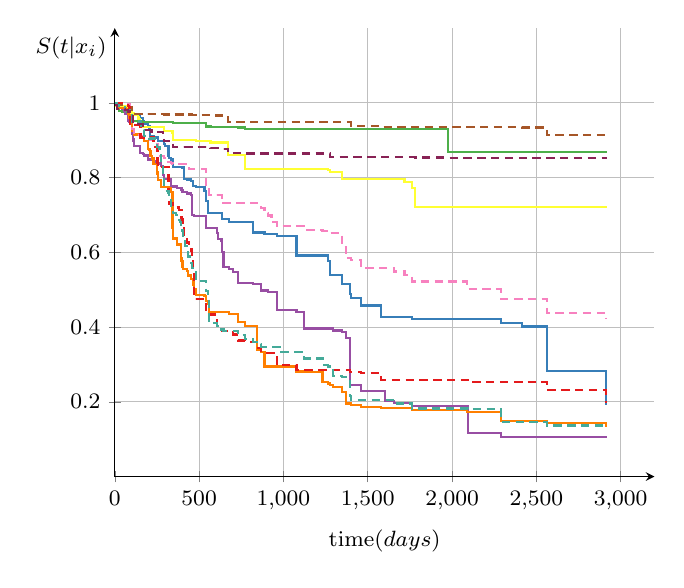
\begin{tikzpicture}[x={(1,0)}]
\footnotesize
\begin{axis}[%
,xlabel=time$(days)$
,ylabel=$S(t|x_i)$
,axis x line = bottom,axis y line = left
,ytick={0.2,0.4,...,1}
,xtick={0,500,1000,...,3000}
,ymax=1.2
,ymin=0
,xmin=0
,xmax=3200
,grid=both
]
%0
\addplot+[const plot, no marks, thick, c1]coordinates {(1.0, 1.0) (7.0, 1.0) (11.0, 1.0) (13.0, 1.0) (26.0, 1.0) (27.0, 0.996) (32.0, 0.996) (42.0, 0.996) (45.0, 0.991) (52.0, 0.991) (56.0, 0.991) (59.0, 0.991) (76.0, 0.9843333333333333) (81.0, 0.9843333333333333) (84.0, 0.9793333333333333) (85.0, 0.9793333333333333) (87.0, 0.9793333333333333) (90.0, 0.9793333333333333) (93.0, 0.9793333333333333) (99.0, 0.9793333333333333) (101.0, 0.9743333333333333) (103.0, 0.9693333333333333) (104.0, 0.9693333333333333) (106.0, 0.9693333333333333) (111.0, 0.9693333333333333) (114.0, 0.9693333333333333) (115.0, 0.9693333333333333) (136.0, 0.9693333333333333) (140.0, 0.9693333333333333) (142.0, 0.9693333333333333) (148.0, 0.9593333333333333) (151.0, 0.9593333333333333) (153.0, 0.9593333333333333) (155.0, 0.9593333333333333) (162.0, 0.9593333333333333) (168.0, 0.9593333333333333) (169.0, 0.9506666666666667) (171.0, 0.9426666666666665) (196.0, 0.9393333333333332) (198.0, 0.9393333333333332) (206.0, 0.9326666666666665) (208.0, 0.9109999999999999) (212.0, 0.9109999999999999) (218.0, 0.9109999999999999) (219.0, 0.9109999999999999) (225.0, 0.9109999999999999) (230.0, 0.9078888888888887) (232.0, 0.9078888888888887) (240.0, 0.9078888888888887) (249.0, 0.9078888888888887) (253.0, 0.9063504273504271) (256.0, 0.8976837606837607) (257.0, 0.8976837606837607) (265.0, 0.8976837606837607) (272.0, 0.8976837606837607) (286.0, 0.8976837606837607) (293.0, 0.891017094017094) (294.0, 0.891017094017094) (296.0, 0.8843504273504275) (318.0, 0.8593504273504273) (322.0, 0.855905982905983) (323.0, 0.8524615384615386) (334.0, 0.8524615384615386) (335.0, 0.8488365384615385) (342.0, 0.8375082417582419) (346.0, 0.8375082417582419) (347.0, 0.8288415750915752) (351.0, 0.8288415750915752) (363.0, 0.8288415750915752) (371.0, 0.8288415750915752) (380.0, 0.8288415750915752) (388.0, 0.8288415750915752) (392.0, 0.8288415750915752) (396.0, 0.8288415750915752) (402.0, 0.8272165750915752) (404.0, 0.8272165750915752) (409.0, 0.8135915750915751) (411.0, 0.7969249084249084) (418.0, 0.7969249084249084) (424.0, 0.7969249084249084) (429.0, 0.7969249084249084) (430.0, 0.7950730565730565) (435.0, 0.7950730565730565) (440.0, 0.7950730565730565) (453.0, 0.7901147232397233) (455.0, 0.7901147232397233) (456.0, 0.7901147232397233) (462.0, 0.7782628713878715) (467.0, 0.7782628713878715) (469.0, 0.7766378713878714) (480.0, 0.7750128713878714) (532.0, 0.7650128713878714) (537.0, 0.7650128713878714) (540.0, 0.7368333842083843) (541.0, 0.7368333842083843) (554.0, 0.7051300875050877) (558.0, 0.7051300875050877) (568.0, 0.7051300875050877) (606.0, 0.7051300875050877) (613.0, 0.7051300875050877) (633.0, 0.7051300875050877) (636.0, 0.6896300875050876) (645.0, 0.6896300875050876) (672.0, 0.6896300875050876) (676.0, 0.6811856430606431) (701.0, 0.6811856430606431) (729.0, 0.6811856430606431) (772.0, 0.6811856430606431) (774.0, 0.6811856430606431) (821.0, 0.6534603683353685) (843.0, 0.6534603683353685) (868.0, 0.6534603683353685) (888.0, 0.6498889397639399) (909.0, 0.6498889397639399) (929.0, 0.6498889397639399) (960.0, 0.6438889397639399) (975.0, 0.6438889397639399) (989.0, 0.6438889397639399) (1077.0, 0.591770112603446) (1124.0, 0.591770112603446) (1231.0, 0.591770112603446) (1265.0, 0.5778812237145572) (1275.0, 0.539881223714557) (1296.0, 0.539881223714557) (1348.0, 0.5162914801248134) (1371.0, 0.5162914801248134) (1393.0, 0.4877200515533848) (1402.0, 0.4777200515533848) (1459.0, 0.4580595577262243) (1579.0, 0.4280595577262244) (1602.0, 0.4280595577262244) (1657.0, 0.4280595577262244) (1718.0, 0.4280595577262244) (1760.0, 0.4213928910595577) (1779.0, 0.4213928910595577) (1977.0, 0.4213928910595577) (2088.0, 0.4213928910595577) (2094.0, 0.4213928910595577) (2289.0, 0.4113928910595577) (2413.0, 0.40139289105955767) (2562.0, 0.28155908289241627) (2911.0, 0.24155908289241626) (2912.0, 0.19223809523809524) };
%1
\addplot+[const plot, no marks, thick, c2]coordinates {(1.0, 0.99901585565883) (7.0, 0.99901585565883) (11.0, 0.99901585565883) (13.0, 0.9910963522823587) (26.0, 0.9910963522823587) (27.0, 0.9777993068079764) (32.0, 0.9777993068079764) (42.0, 0.9777993068079764) (45.0, 0.975394934570947) (52.0, 0.975394934570947) (56.0, 0.975394934570947) (59.0, 0.975394934570947) (76.0, 0.9752018555552513) (81.0, 0.9752018555552513) (84.0, 0.9696462999996958) (85.0, 0.9682039923073882) (87.0, 0.9682039923073882) (90.0, 0.9682039923073882) (93.0, 0.9682039923073882) (99.0, 0.968004879572452) (101.0, 0.968004879572452) (103.0, 0.9678057668375157) (104.0, 0.9678057668375157) (106.0, 0.9520989186461472) (111.0, 0.9513247250977601) (114.0, 0.9513247250977601) (115.0, 0.9513247250977601) (136.0, 0.950550531549373) (140.0, 0.950550531549373) (142.0, 0.950550531549373) (148.0, 0.950550531549373) (151.0, 0.950550531549373) (153.0, 0.950550531549373) (155.0, 0.950550531549373) (162.0, 0.9495772252660497) (168.0, 0.9486039189827263) (169.0, 0.9486039189827263) (171.0, 0.9486039189827263) (196.0, 0.9486039189827263) (198.0, 0.9486039189827263) (206.0, 0.9486039189827263) (208.0, 0.9484003815203471) (212.0, 0.9484003815203471) (218.0, 0.9481968440579679) (219.0, 0.9481968440579679) (225.0, 0.9481968440579679) (230.0, 0.9481968440579679) (232.0, 0.9481968440579679) (240.0, 0.9481968440579679) (249.0, 0.9481968440579679) (253.0, 0.9481968440579679) (256.0, 0.9481968440579679) (257.0, 0.9481968440579679) (265.0, 0.9481968440579679) (272.0, 0.9481968440579679) (286.0, 0.9481968440579679) (293.0, 0.9479933065955887) (294.0, 0.9479933065955887) (296.0, 0.9479933065955887) (318.0, 0.9479933065955887) (322.0, 0.9479933065955887) (323.0, 0.9479933065955887) (334.0, 0.9479933065955887) (335.0, 0.9479933065955887) (342.0, 0.9479933065955887) (346.0, 0.9470132088701435) (347.0, 0.9470132088701435) (351.0, 0.9470132088701435) (363.0, 0.9470132088701435) (371.0, 0.9470132088701435) (380.0, 0.9470132088701435) (388.0, 0.9470132088701435) (392.0, 0.9470132088701435) (396.0, 0.9470132088701435) (402.0, 0.9470132088701435) (404.0, 0.9470132088701435) (409.0, 0.9470132088701435) (411.0, 0.9470132088701435) (418.0, 0.9470132088701435) (424.0, 0.9470132088701435) (429.0, 0.9470132088701435) (430.0, 0.9470132088701435) (435.0, 0.9470132088701435) (440.0, 0.9470132088701435) (453.0, 0.9470132088701435) (455.0, 0.9470132088701435) (456.0, 0.9470132088701435) (462.0, 0.9470132088701435) (467.0, 0.9470132088701435) (469.0, 0.9470132088701435) (480.0, 0.9470132088701435) (532.0, 0.9470132088701435) (537.0, 0.9470132088701435) (540.0, 0.9370132088701435) (541.0, 0.9370132088701435) (554.0, 0.9370132088701435) (558.0, 0.9370132088701435) (568.0, 0.9362276527441736) (606.0, 0.9362276527441736) (613.0, 0.9362276527441736) (633.0, 0.9362276527441736) (636.0, 0.9362276527441736) (645.0, 0.9362276527441736) (672.0, 0.9360141837401436) (676.0, 0.9360141837401436) (701.0, 0.9360141837401436) (729.0, 0.9344757222016821) (772.0, 0.9344757222016821) (774.0, 0.9311484399472492) (821.0, 0.9311484399472492) (843.0, 0.9311484399472492) (868.0, 0.9311484399472492) (888.0, 0.9311484399472492) (909.0, 0.9311484399472492) (929.0, 0.9311484399472492) (960.0, 0.9311484399472492) (975.0, 0.9311484399472492) (989.0, 0.9311484399472492) (1077.0, 0.9311484399472492) (1124.0, 0.9311484399472492) (1231.0, 0.9311484399472492) (1265.0, 0.9311484399472492) (1275.0, 0.9311484399472492) (1296.0, 0.9311484399472492) (1348.0, 0.9311484399472492) (1371.0, 0.9311484399472492) (1393.0, 0.9311484399472492) (1402.0, 0.9305737495447723) (1459.0, 0.9305737495447723) (1579.0, 0.9305737495447723) (1602.0, 0.9305737495447723) (1657.0, 0.9305737495447723) (1718.0, 0.9305737495447723) (1760.0, 0.9305737495447723) (1779.0, 0.9303220876167263) (1977.0, 0.8694718846293977) (2088.0, 0.8694718846293977) (2094.0, 0.8694718846293977) (2289.0, 0.8694718846293977) (2413.0, 0.8690132255438731) (2562.0, 0.8690132255438731) (2911.0, 0.8690132255438731) (2912.0, 0.8690132255438731) };
%2
\addplot+[const plot, no marks, thick, c3]coordinates {(1.0, 1.0) (7.0, 1.0) (11.0, 0.9966666666666666) (13.0, 0.9966666666666666) (26.0, 0.9966666666666666) (27.0, 0.9966666666666666) (32.0, 0.9966666666666666) (42.0, 0.9849999999999999) (45.0, 0.9849999999999999) (52.0, 0.9849999999999999) (56.0, 0.9799999999999999) (59.0, 0.9708333333333333) (76.0, 0.9643333333333333) (81.0, 0.9523333333333333) (84.0, 0.9523333333333333) (85.0, 0.9523333333333333) (87.0, 0.9505151515151513) (90.0, 0.9505151515151513) (93.0, 0.9438484848484847) (99.0, 0.9438484848484847) (101.0, 0.9263484848484849) (103.0, 0.9178636363636363) (104.0, 0.9178636363636363) (106.0, 0.904530303030303) (111.0, 0.8978636363636363) (114.0, 0.884530303030303) (115.0, 0.884530303030303) (136.0, 0.884530303030303) (140.0, 0.884530303030303) (142.0, 0.884530303030303) (148.0, 0.8711969696969697) (151.0, 0.8658636363636364) (153.0, 0.8658636363636364) (155.0, 0.8658636363636364) (162.0, 0.8658636363636364) (168.0, 0.8658636363636364) (169.0, 0.8625303030303031) (171.0, 0.8591969696969697) (196.0, 0.848525974025974) (198.0, 0.848525974025974) (206.0, 0.848525974025974) (208.0, 0.848525974025974) (212.0, 0.848525974025974) (218.0, 0.848525974025974) (219.0, 0.848525974025974) (225.0, 0.848525974025974) (230.0, 0.8447759740259739) (232.0, 0.8447759740259739) (240.0, 0.8381093073593072) (249.0, 0.8381093073593072) (253.0, 0.8381093073593072) (256.0, 0.8381093073593072) (257.0, 0.8381093073593072) (265.0, 0.8381093073593072) (272.0, 0.8314426406926407) (286.0, 0.8081093073593074) (293.0, 0.8041093073593075) (294.0, 0.7974426406926408) (296.0, 0.7974426406926408) (318.0, 0.7974426406926408) (322.0, 0.7974426406926408) (323.0, 0.7974426406926408) (334.0, 0.7794426406926407) (335.0, 0.7761093073593073) (342.0, 0.7761093073593073) (346.0, 0.7761093073593073) (347.0, 0.7761093073593073) (351.0, 0.7761093073593073) (363.0, 0.7761093073593073) (371.0, 0.772775974025974) (380.0, 0.772775974025974) (388.0, 0.772775974025974) (392.0, 0.772775974025974) (396.0, 0.7661093073593074) (402.0, 0.7611093073593074) (404.0, 0.7611093073593074) (409.0, 0.7611093073593074) (411.0, 0.7611093073593074) (418.0, 0.7611093073593074) (424.0, 0.7611093073593074) (429.0, 0.7611093073593074) (430.0, 0.7577759740259741) (435.0, 0.7577759740259741) (440.0, 0.7577759740259741) (453.0, 0.7527759740259741) (455.0, 0.7527759740259741) (456.0, 0.7007759740259739) (462.0, 0.7007759740259739) (467.0, 0.7007759740259739) (469.0, 0.6974426406926405) (480.0, 0.6974426406926405) (532.0, 0.6974426406926405) (537.0, 0.6974426406926405) (540.0, 0.6749426406926406) (541.0, 0.6654707792207794) (554.0, 0.6654707792207794) (558.0, 0.6654707792207794) (568.0, 0.6654707792207794) (606.0, 0.6509989177489176) (613.0, 0.636832251082251) (633.0, 0.631832251082251) (636.0, 0.6018322510822511) (645.0, 0.5614989177489178) (672.0, 0.5614989177489178) (676.0, 0.5548322510822511) (701.0, 0.5481655844155844) (729.0, 0.5181655844155845) (772.0, 0.5181655844155845) (774.0, 0.5181655844155845) (821.0, 0.5148322510822512) (843.0, 0.5148322510822512) (868.0, 0.4981655844155845) (888.0, 0.4981655844155845) (909.0, 0.4931655844155845) (929.0, 0.4931655844155845) (960.0, 0.44483225108225105) (975.0, 0.44483225108225105) (989.0, 0.44483225108225105) (1077.0, 0.43983225108225105) (1124.0, 0.39608225108225115) (1231.0, 0.39608225108225115) (1265.0, 0.39608225108225115) (1275.0, 0.39608225108225115) (1296.0, 0.39108225108225114) (1348.0, 0.38687445887445887) (1371.0, 0.37124945887445887) (1393.0, 0.24591666666666667) (1402.0, 0.24591666666666667) (1459.0, 0.22925000000000004) (1579.0, 0.22925000000000004) (1602.0, 0.20258333333333337) (1657.0, 0.19591666666666668) (1718.0, 0.19591666666666668) (1760.0, 0.18925) (1779.0, 0.18925) (1977.0, 0.18925) (2088.0, 0.18925) (2094.0, 0.11625) (2289.0, 0.10500000000000002) (2413.0, 0.10500000000000002) (2562.0, 0.10500000000000002) (2911.0, 0.10500000000000002) (2912.0, 0.10500000000000002) };
%3
\addplot+[const plot, no marks, thick, c4]coordinates {(1.0, 1.0) (7.0, 1.0) (11.0, 1.0) (13.0, 1.0) (26.0, 0.986) (27.0, 0.986) (32.0, 0.986) (42.0, 0.986) (45.0, 0.986) (52.0, 0.986) (56.0, 0.986) (59.0, 0.986) (76.0, 0.9701818181818183) (81.0, 0.9701818181818183) (84.0, 0.9701818181818183) (85.0, 0.9701818181818183) (87.0, 0.960348484848485) (90.0, 0.9538484848484851) (93.0, 0.9538484848484851) (99.0, 0.9520303030303032) (101.0, 0.9420303030303032) (103.0, 0.9253636363636365) (104.0, 0.9253636363636365) (106.0, 0.9253636363636365) (111.0, 0.9253636363636365) (114.0, 0.9153636363636365) (115.0, 0.9153636363636365) (136.0, 0.9153636363636365) (140.0, 0.9153636363636365) (142.0, 0.9153636363636365) (148.0, 0.9153636363636365) (151.0, 0.9153636363636365) (153.0, 0.9051731601731601) (155.0, 0.9051731601731601) (162.0, 0.9051731601731601) (168.0, 0.9051731601731601) (169.0, 0.9051731601731601) (171.0, 0.8971731601731602) (196.0, 0.8770286380286381) (198.0, 0.8770286380286381) (206.0, 0.874528638028638) (208.0, 0.8711953046953046) (212.0, 0.8578619713619713) (218.0, 0.8578619713619713) (219.0, 0.8511953046953046) (225.0, 0.8511953046953046) (230.0, 0.8356707736707736) (232.0, 0.8356707736707736) (240.0, 0.8356707736707736) (249.0, 0.8150041070041071) (253.0, 0.8100041070041071) (256.0, 0.8100041070041071) (257.0, 0.7933374403374404) (265.0, 0.7933374403374404) (272.0, 0.7751707736707736) (286.0, 0.7751707736707736) (293.0, 0.7751707736707736) (294.0, 0.7751707736707736) (296.0, 0.7751707736707736) (318.0, 0.7751707736707736) (322.0, 0.7737263292263292) (323.0, 0.7722818847818848) (334.0, 0.7722818847818848) (335.0, 0.7616568847818848) (342.0, 0.6654184981684982) (346.0, 0.6654184981684982) (347.0, 0.6370851648351649) (351.0, 0.6370851648351649) (363.0, 0.6370851648351649) (371.0, 0.6212401764901766) (380.0, 0.6212401764901766) (388.0, 0.6212401764901766) (392.0, 0.5854068431568433) (396.0, 0.5759876512376515) (402.0, 0.5614462343212344) (404.0, 0.5564462343212344) (409.0, 0.5548212343212344) (411.0, 0.5548212343212344) (418.0, 0.5548212343212344) (424.0, 0.5548212343212344) (429.0, 0.551487900987901) (430.0, 0.5498095793095793) (435.0, 0.5381429126429126) (440.0, 0.5381429126429126) (453.0, 0.5281845793095793) (455.0, 0.5281845793095793) (456.0, 0.5281845793095793) (462.0, 0.519839590964591) (467.0, 0.5131729242979243) (469.0, 0.5025479242979243) (480.0, 0.4856350455100455) (532.0, 0.48230171217671214) (537.0, 0.48230171217671214) (540.0, 0.48230171217671214) (541.0, 0.46896837884337883) (554.0, 0.4628708652458653) (558.0, 0.4407758769008769) (568.0, 0.4407758769008769) (606.0, 0.4407758769008769) (613.0, 0.4407758769008769) (633.0, 0.4407758769008769) (636.0, 0.4407758769008769) (645.0, 0.4407758769008769) (672.0, 0.4407758769008769) (676.0, 0.43410921023421023) (701.0, 0.43410921023421023) (729.0, 0.41344254356754356) (772.0, 0.40844254356754356) (774.0, 0.40344254356754355) (821.0, 0.40344254356754355) (843.0, 0.3398592102342103) (868.0, 0.3331925435675436) (888.0, 0.294621114996115) (909.0, 0.294621114996115) (929.0, 0.294621114996115) (960.0, 0.294621114996115) (975.0, 0.294621114996115) (989.0, 0.294621114996115) (1077.0, 0.28132944832944834) (1124.0, 0.2790916860916861) (1231.0, 0.25259168609168614) (1265.0, 0.24880380730380733) (1275.0, 0.24501592851592854) (1296.0, 0.24001592851592854) (1348.0, 0.22554040404040404) (1371.0, 0.19554040404040404) (1393.0, 0.19554040404040404) (1402.0, 0.19154040404040404) (1459.0, 0.18654040404040406) (1579.0, 0.18320707070707073) (1602.0, 0.18320707070707073) (1657.0, 0.18320707070707073) (1718.0, 0.18320707070707073) (1760.0, 0.17820707070707073) (1779.0, 0.17820707070707073) (1977.0, 0.17820707070707073) (2088.0, 0.17320707070707073) (2094.0, 0.17320707070707073) (2289.0, 0.14954040404040403) (2413.0, 0.14954040404040403) (2562.0, 0.14354040404040405) (2911.0, 0.13604040404040404) (2912.0, 0.13604040404040404) };
%4
\addplot+[const plot, no marks, thick, c5]coordinates {(1.0, 0.9914200530937309) (7.0, 0.9914200530937309) (11.0, 0.9914200530937309) (13.0, 0.9912490877289557) (26.0, 0.9912490877289557) (27.0, 0.9910020997771484) (32.0, 0.9910020997771484) (42.0, 0.9910020997771484) (45.0, 0.9908199497623411) (52.0, 0.9908199497623411) (56.0, 0.9908199497623411) (59.0, 0.9908199497623411) (76.0, 0.9906268707466456) (81.0, 0.9906268707466456) (84.0, 0.9759602040799789) (85.0, 0.9759602040799789) (87.0, 0.9759602040799789) (90.0, 0.9759602040799789) (93.0, 0.9759602040799789) (99.0, 0.9736756211954529) (101.0, 0.9724991506072176) (103.0, 0.9723000378722815) (104.0, 0.9723000378722815) (106.0, 0.9723000378722815) (111.0, 0.9683000378722815) (114.0, 0.9683000378722815) (115.0, 0.9683000378722815) (136.0, 0.961633371205615) (140.0, 0.9576333712056149) (142.0, 0.9576333712056149) (148.0, 0.9576333712056149) (151.0, 0.9426333712056149) (153.0, 0.9426333712056149) (155.0, 0.9426333712056149) (162.0, 0.9424342584706786) (168.0, 0.9353011907376678) (169.0, 0.9353011907376678) (171.0, 0.9353011907376678) (196.0, 0.9353011907376678) (198.0, 0.9353011907376678) (206.0, 0.9353011907376678) (208.0, 0.9350976532752885) (212.0, 0.9350976532752885) (218.0, 0.9346230090767672) (219.0, 0.9346230090767672) (225.0, 0.9346230090767672) (230.0, 0.9346230090767672) (232.0, 0.9346230090767672) (240.0, 0.9346230090767672) (249.0, 0.9346230090767672) (253.0, 0.9346230090767672) (256.0, 0.9346230090767672) (257.0, 0.9346230090767672) (265.0, 0.9346230090767672) (272.0, 0.9346230090767672) (286.0, 0.9346230090767672) (293.0, 0.9241483648782457) (294.0, 0.9241483648782457) (296.0, 0.9241483648782457) (318.0, 0.9241483648782457) (322.0, 0.9241483648782457) (323.0, 0.9241483648782457) (334.0, 0.9241483648782457) (335.0, 0.9241483648782457) (342.0, 0.9211180618479428) (346.0, 0.9017692560629476) (347.0, 0.9017692560629476) (351.0, 0.9017692560629476) (363.0, 0.9017692560629476) (371.0, 0.9017692560629476) (380.0, 0.9017692560629476) (388.0, 0.9017692560629476) (392.0, 0.9017692560629476) (396.0, 0.9017692560629476) (402.0, 0.9017692560629476) (404.0, 0.9017692560629476) (409.0, 0.9017692560629476) (411.0, 0.9017692560629476) (418.0, 0.9017692560629476) (424.0, 0.9017692560629476) (429.0, 0.9017692560629476) (430.0, 0.9017692560629476) (435.0, 0.9017692560629476) (440.0, 0.9017692560629476) (453.0, 0.9017692560629476) (455.0, 0.9017692560629476) (456.0, 0.9017692560629476) (462.0, 0.9017692560629476) (467.0, 0.9017692560629476) (469.0, 0.9017692560629476) (480.0, 0.8979813772750689) (532.0, 0.8979813772750689) (537.0, 0.8979813772750689) (540.0, 0.8979813772750689) (541.0, 0.8979813772750689) (554.0, 0.8979813772750689) (558.0, 0.8979813772750689) (568.0, 0.8939568355991515) (606.0, 0.8939568355991515) (613.0, 0.8939568355991515) (633.0, 0.8939568355991515) (636.0, 0.8939568355991515) (645.0, 0.8939568355991515) (672.0, 0.8612630239760308) (676.0, 0.8612630239760308) (701.0, 0.8612630239760308) (729.0, 0.8612630239760308) (772.0, 0.8612630239760308) (774.0, 0.8237245348932501) (821.0, 0.8237245348932501) (843.0, 0.8237245348932501) (868.0, 0.8237245348932501) (888.0, 0.8237245348932501) (909.0, 0.8237245348932501) (929.0, 0.8237245348932501) (960.0, 0.8237245348932501) (975.0, 0.8237245348932501) (989.0, 0.8237245348932501) (1077.0, 0.8237245348932501) (1124.0, 0.8237245348932501) (1231.0, 0.8237245348932501) (1265.0, 0.8199366561053713) (1275.0, 0.8161487773174925) (1296.0, 0.8161487773174925) (1348.0, 0.7961487773174925) (1371.0, 0.7961487773174925) (1393.0, 0.7961487773174925) (1402.0, 0.7961487773174925) (1459.0, 0.7961487773174925) (1579.0, 0.7961487773174925) (1602.0, 0.7961487773174925) (1657.0, 0.7961487773174925) (1718.0, 0.7884821106508259) (1760.0, 0.7731487773174925) (1779.0, 0.7218464094281226) (1977.0, 0.7218464094281226) (2088.0, 0.7218464094281226) (2094.0, 0.7218464094281226) (2289.0, 0.7218464094281226) (2413.0, 0.7218464094281226) (2562.0, 0.7218464094281226) (2911.0, 0.7218464094281226) (2912.0, 0.7218464094281226) };
%5
\addplot+[const plot, no marks, thick, c6]coordinates {(1.0, 0.9944200530937308) (7.0, 0.9944200530937308) (11.0, 0.9944200530937308) (13.0, 0.9942490877289556) (26.0, 0.9942490877289556) (27.0, 0.9937035923144619) (32.0, 0.9937035923144619) (42.0, 0.9937035923144619) (45.0, 0.9935214422996546) (52.0, 0.9935214422996546) (56.0, 0.9935214422996546) (59.0, 0.9935214422996546) (76.0, 0.993328363283959) (81.0, 0.993328363283959) (84.0, 0.993328363283959) (85.0, 0.988328363283959) (87.0, 0.988328363283959) (90.0, 0.988328363283959) (93.0, 0.988328363283959) (99.0, 0.9713619622176151) (101.0, 0.9713619622176151) (103.0, 0.971162849482679) (104.0, 0.971162849482679) (106.0, 0.971162849482679) (111.0, 0.971162849482679) (114.0, 0.971162849482679) (115.0, 0.971162849482679) (136.0, 0.971162849482679) (140.0, 0.971162849482679) (142.0, 0.971162849482679) (148.0, 0.971162849482679) (151.0, 0.971162849482679) (153.0, 0.971162849482679) (155.0, 0.971162849482679) (162.0, 0.9709637367477427) (168.0, 0.9704973356813986) (169.0, 0.9704973356813986) (171.0, 0.9704973356813986) (196.0, 0.9704973356813986) (198.0, 0.9704973356813986) (206.0, 0.9704973356813986) (208.0, 0.9702937982190193) (212.0, 0.9702937982190193) (218.0, 0.9698191540204979) (219.0, 0.9698191540204979) (225.0, 0.9698191540204979) (230.0, 0.9698191540204979) (232.0, 0.9698191540204979) (240.0, 0.9698191540204979) (249.0, 0.9698191540204979) (253.0, 0.9698191540204979) (256.0, 0.9698191540204979) (257.0, 0.9698191540204979) (265.0, 0.9698191540204979) (272.0, 0.9698191540204979) (286.0, 0.9698191540204979) (293.0, 0.9693445098219765) (294.0, 0.9693445098219765) (296.0, 0.9693445098219765) (318.0, 0.9693445098219765) (322.0, 0.9693445098219765) (323.0, 0.9693445098219765) (334.0, 0.9693445098219765) (335.0, 0.9693445098219765) (342.0, 0.9693445098219765) (346.0, 0.9688674989087761) (347.0, 0.9688674989087761) (351.0, 0.9688674989087761) (363.0, 0.9688674989087761) (371.0, 0.9688674989087761) (380.0, 0.9688674989087761) (388.0, 0.9688674989087761) (392.0, 0.9688674989087761) (396.0, 0.9688674989087761) (402.0, 0.9688674989087761) (404.0, 0.9688674989087761) (409.0, 0.9688674989087761) (411.0, 0.9688674989087761) (418.0, 0.9688674989087761) (424.0, 0.9688674989087761) (429.0, 0.9688674989087761) (430.0, 0.9688674989087761) (435.0, 0.9688674989087761) (440.0, 0.9688674989087761) (453.0, 0.9688674989087761) (455.0, 0.9668674989087761) (456.0, 0.9668674989087761) (462.0, 0.9668674989087761) (467.0, 0.9668674989087761) (469.0, 0.9668674989087761) (480.0, 0.9668674989087761) (532.0, 0.9668674989087761) (537.0, 0.9668674989087761) (540.0, 0.9668674989087761) (541.0, 0.9668674989087761) (554.0, 0.9668674989087761) (558.0, 0.9668674989087761) (568.0, 0.9663814187713203) (606.0, 0.9663814187713203) (613.0, 0.9663814187713203) (633.0, 0.9663814187713203) (636.0, 0.9663814187713203) (645.0, 0.9663814187713203) (672.0, 0.949226068686661) (676.0, 0.949226068686661) (701.0, 0.949226068686661) (729.0, 0.949226068686661) (772.0, 0.949226068686661) (774.0, 0.9487303146466155) (821.0, 0.9487303146466155) (843.0, 0.9487303146466155) (868.0, 0.9487303146466155) (888.0, 0.9487303146466155) (909.0, 0.9487303146466155) (929.0, 0.9487303146466155) (960.0, 0.9487303146466155) (975.0, 0.9487303146466155) (989.0, 0.9487303146466155) (1077.0, 0.9487303146466155) (1124.0, 0.9487303146466155) (1231.0, 0.9487303146466155) (1265.0, 0.9487303146466155) (1275.0, 0.9487303146466155) (1296.0, 0.9487303146466155) (1348.0, 0.9487303146466155) (1371.0, 0.9487303146466155) (1393.0, 0.9487303146466155) (1402.0, 0.938658886075187) (1459.0, 0.938658886075187) (1579.0, 0.9355731717894727) (1602.0, 0.9355731717894727) (1657.0, 0.9355731717894727) (1718.0, 0.9355731717894727) (1760.0, 0.9355731717894727) (1779.0, 0.9349944506237498) (1977.0, 0.934556639678476) (2088.0, 0.934556639678476) (2094.0, 0.934556639678476) (2289.0, 0.934556639678476) (2413.0, 0.9340979805929512) (2562.0, 0.9140979805929512) (2911.0, 0.9140979805929512) (2912.0, 0.9140979805929512) };
%6
\addplot+[const plot, no marks, thick, c7]coordinates {(1.0, 1.0) (7.0, 1.0) (11.0, 1.0) (13.0, 1.0) (26.0, 1.0) (27.0, 1.0) (32.0, 1.0) (42.0, 1.0) (45.0, 0.996) (52.0, 0.996) (56.0, 0.996) (59.0, 0.996) (76.0, 0.996) (81.0, 0.996) (84.0, 0.996) (85.0, 0.996) (87.0, 0.996) (90.0, 0.9776666666666667) (93.0, 0.9776666666666667) (99.0, 0.9776666666666667) (101.0, 0.9660000000000001) (103.0, 0.9359999999999999) (104.0, 0.9293333333333332) (106.0, 0.9293333333333332) (111.0, 0.9293333333333332) (114.0, 0.9159999999999999) (115.0, 0.9159999999999999) (136.0, 0.9135) (140.0, 0.9135) (142.0, 0.9135) (148.0, 0.9135) (151.0, 0.9119615384615384) (153.0, 0.9119615384615384) (155.0, 0.9119615384615384) (162.0, 0.9119615384615384) (168.0, 0.9119615384615384) (169.0, 0.9119615384615384) (171.0, 0.9119615384615384) (196.0, 0.9119615384615384) (198.0, 0.9119615384615384) (206.0, 0.9052948717948717) (208.0, 0.9002948717948717) (212.0, 0.9002948717948717) (218.0, 0.9002948717948717) (219.0, 0.9002948717948717) (225.0, 0.9002948717948717) (230.0, 0.9002948717948717) (232.0, 0.893628205128205) (240.0, 0.893628205128205) (249.0, 0.893628205128205) (253.0, 0.8587564102564101) (256.0, 0.8587564102564101) (257.0, 0.8587564102564101) (265.0, 0.8587564102564101) (272.0, 0.8587564102564101) (286.0, 0.8587564102564101) (293.0, 0.8587564102564101) (294.0, 0.8520897435897435) (296.0, 0.8417564102564102) (318.0, 0.8417564102564102) (322.0, 0.8417564102564102) (323.0, 0.8417564102564102) (334.0, 0.8400641025641026) (335.0, 0.8400641025641026) (342.0, 0.8360641025641026) (346.0, 0.8360641025641026) (347.0, 0.8360641025641026) (351.0, 0.8360641025641026) (363.0, 0.8360641025641026) (371.0, 0.8360641025641026) (380.0, 0.8360641025641026) (388.0, 0.8360641025641026) (392.0, 0.8360641025641026) (396.0, 0.8360641025641026) (402.0, 0.8360641025641026) (404.0, 0.8360641025641026) (409.0, 0.8360641025641026) (411.0, 0.8360641025641026) (418.0, 0.8360641025641026) (424.0, 0.8360641025641026) (429.0, 0.8360641025641026) (430.0, 0.8360641025641026) (435.0, 0.8293974358974359) (440.0, 0.8227307692307692) (453.0, 0.8227307692307692) (455.0, 0.8227307692307692) (456.0, 0.8227307692307692) (462.0, 0.8227307692307692) (467.0, 0.8227307692307692) (469.0, 0.8227307692307692) (480.0, 0.8227307692307692) (532.0, 0.8227307692307692) (537.0, 0.8227307692307692) (540.0, 0.7927307692307691) (541.0, 0.7684935897435898) (554.0, 0.7684935897435898) (558.0, 0.7534935897435899) (568.0, 0.7534935897435899) (606.0, 0.7534935897435899) (613.0, 0.7534935897435899) (633.0, 0.7534935897435899) (636.0, 0.7459935897435899) (645.0, 0.7319935897435899) (672.0, 0.7319935897435899) (676.0, 0.7319935897435899) (701.0, 0.7319935897435899) (729.0, 0.7319935897435899) (772.0, 0.7319935897435899) (774.0, 0.7319935897435899) (821.0, 0.7319935897435899) (843.0, 0.7253269230769231) (868.0, 0.7186602564102565) (888.0, 0.7053269230769232) (909.0, 0.6986602564102565) (929.0, 0.6807435897435898) (960.0, 0.6707435897435897) (975.0, 0.6707435897435897) (989.0, 0.6707435897435897) (1077.0, 0.6707435897435897) (1124.0, 0.6607435897435897) (1231.0, 0.6578269230769231) (1265.0, 0.6578269230769231) (1275.0, 0.6511602564102564) (1296.0, 0.6511602564102564) (1348.0, 0.6144935897435897) (1371.0, 0.5853269230769231) (1393.0, 0.5853269230769231) (1402.0, 0.5786602564102564) (1459.0, 0.5586602564102564) (1579.0, 0.5586602564102564) (1602.0, 0.5586602564102564) (1657.0, 0.5486602564102564) (1718.0, 0.5386602564102564) (1760.0, 0.5219935897435897) (1779.0, 0.5219935897435897) (1977.0, 0.5219935897435897) (2088.0, 0.5019935897435897) (2094.0, 0.5019935897435897) (2289.0, 0.47532692307692304) (2413.0, 0.47532692307692304) (2562.0, 0.437826923076923) (2911.0, 0.437826923076923) (2912.0, 0.42449358974358964) };
%7
\addplot+[const plot, no marks, thick, c8]coordinates {(1.0, 1.0) (7.0, 1.0) (11.0, 1.0) (13.0, 1.0) (26.0, 1.0) (27.0, 1.0) (32.0, 1.0) (42.0, 1.0) (45.0, 1.0) (52.0, 1.0) (56.0, 1.0) (59.0, 1.0) (76.0, 0.9926666666666667) (81.0, 0.9926666666666667) (84.0, 0.9926666666666667) (85.0, 0.9876666666666667) (87.0, 0.9843333333333334) (90.0, 0.944) (93.0, 0.944) (99.0, 0.944) (101.0, 0.944) (103.0, 0.944) (104.0, 0.944) (106.0, 0.944) (111.0, 0.944) (114.0, 0.9406666666666667) (115.0, 0.9406666666666667) (136.0, 0.9406666666666667) (140.0, 0.9406666666666667) (142.0, 0.9406666666666667) (148.0, 0.9366666666666665) (151.0, 0.9366666666666665) (153.0, 0.9076666666666664) (155.0, 0.9076666666666664) (162.0, 0.9076666666666664) (168.0, 0.9076666666666664) (169.0, 0.9076666666666664) (171.0, 0.9076666666666664) (196.0, 0.9076666666666664) (198.0, 0.9076666666666664) (206.0, 0.9076666666666664) (208.0, 0.9076666666666664) (212.0, 0.9076666666666664) (218.0, 0.9076666666666664) (219.0, 0.9076666666666664) (225.0, 0.9076666666666664) (230.0, 0.8826190476190474) (232.0, 0.8826190476190474) (240.0, 0.8826190476190474) (249.0, 0.8826190476190474) (253.0, 0.8383412698412698) (256.0, 0.8343412698412698) (257.0, 0.8343412698412698) (265.0, 0.8343412698412698) (272.0, 0.8276746031746031) (286.0, 0.8276746031746031) (293.0, 0.8276746031746031) (294.0, 0.8276746031746031) (296.0, 0.8276746031746031) (318.0, 0.7628174603174602) (322.0, 0.7461507936507935) (323.0, 0.7309603174603175) (334.0, 0.7309603174603175) (335.0, 0.7309603174603175) (342.0, 0.7219603174603175) (346.0, 0.7219603174603175) (347.0, 0.7202936507936508) (351.0, 0.7202936507936508) (363.0, 0.7202936507936508) (371.0, 0.7202936507936508) (380.0, 0.7136269841269842) (388.0, 0.7136269841269842) (392.0, 0.7136269841269842) (396.0, 0.6883234126984128) (402.0, 0.6636448412698414) (404.0, 0.6636448412698414) (409.0, 0.6551031746031747) (411.0, 0.638436507936508) (418.0, 0.638436507936508) (424.0, 0.638436507936508) (429.0, 0.638436507936508) (430.0, 0.6265846560846562) (435.0, 0.6265846560846562) (440.0, 0.6199179894179896) (453.0, 0.6199179894179896) (455.0, 0.6049179894179896) (456.0, 0.5821560846560847) (462.0, 0.5429708994708995) (467.0, 0.5429708994708995) (469.0, 0.4753518518518519) (480.0, 0.4753518518518519) (532.0, 0.4753518518518519) (537.0, 0.4753518518518519) (540.0, 0.4338518518518519) (541.0, 0.4338518518518519) (554.0, 0.4338518518518519) (558.0, 0.4338518518518519) (568.0, 0.4338518518518519) (606.0, 0.393774470899471) (613.0, 0.393774470899471) (633.0, 0.393774470899471) (636.0, 0.39044113756613763) (645.0, 0.39044113756613763) (672.0, 0.39044113756613763) (676.0, 0.39044113756613763) (701.0, 0.3804411375661376) (729.0, 0.3642506613756613) (772.0, 0.36091732804232807) (774.0, 0.36091732804232807) (821.0, 0.36091732804232807) (843.0, 0.34425066137566135) (868.0, 0.33072685185185186) (888.0, 0.33072685185185186) (909.0, 0.33072685185185186) (929.0, 0.33072685185185186) (960.0, 0.29906018518518523) (975.0, 0.29906018518518523) (989.0, 0.29906018518518523) (1077.0, 0.28489969135802473) (1124.0, 0.28489969135802473) (1231.0, 0.28489969135802473) (1265.0, 0.28489969135802473) (1275.0, 0.28489969135802473) (1296.0, 0.28489969135802473) (1348.0, 0.28489969135802473) (1371.0, 0.28489969135802473) (1393.0, 0.2795663580246914) (1402.0, 0.2795663580246914) (1459.0, 0.2774058641975309) (1579.0, 0.25938503086419756) (1602.0, 0.25938503086419756) (1657.0, 0.25938503086419756) (1718.0, 0.25938503086419756) (1760.0, 0.25938503086419756) (1779.0, 0.25938503086419756) (1977.0, 0.25938503086419756) (2088.0, 0.25938503086419756) (2094.0, 0.25271836419753085) (2289.0, 0.25271836419753085) (2413.0, 0.25271836419753085) (2562.0, 0.23173070987654323) (2911.0, 0.23173070987654323) (2912.0, 0.1956666666666667) };
%8
\addplot+[const plot, no marks, thick, c9]coordinates {(1.0, 1.0) (7.0, 1.0) (11.0, 0.9933333333333333) (13.0, 0.9933333333333333) (26.0, 0.9883333333333333) (27.0, 0.9883333333333333) (32.0, 0.9883333333333333) (42.0, 0.9883333333333333) (45.0, 0.9883333333333333) (52.0, 0.9883333333333333) (56.0, 0.9883333333333333) (59.0, 0.9816666666666667) (76.0, 0.9816666666666667) (81.0, 0.9816666666666667) (84.0, 0.9816666666666667) (85.0, 0.9816666666666667) (87.0, 0.9763095238095238) (90.0, 0.9738095238095238) (93.0, 0.9738095238095238) (99.0, 0.971991341991342) (101.0, 0.9503246753246752) (103.0, 0.9503246753246752) (104.0, 0.9503246753246752) (106.0, 0.9503246753246752) (111.0, 0.9503246753246752) (114.0, 0.9503246753246752) (115.0, 0.9503246753246752) (136.0, 0.9503246753246752) (140.0, 0.9503246753246752) (142.0, 0.9503246753246752) (148.0, 0.9503246753246752) (151.0, 0.9503246753246752) (153.0, 0.9503246753246752) (155.0, 0.9378246753246752) (162.0, 0.9378246753246752) (168.0, 0.9378246753246752) (169.0, 0.9283008658008656) (171.0, 0.9121103896103895) (196.0, 0.9105719280719279) (198.0, 0.9105719280719279) (206.0, 0.9046433566433565) (208.0, 0.9046433566433565) (212.0, 0.9046433566433565) (218.0, 0.9046433566433565) (219.0, 0.9046433566433565) (225.0, 0.9046433566433565) (230.0, 0.9046433566433565) (232.0, 0.9046433566433565) (240.0, 0.8878814518814516) (249.0, 0.8828814518814516) (253.0, 0.8828814518814516) (256.0, 0.8828814518814516) (257.0, 0.8828814518814516) (265.0, 0.8687147852147852) (272.0, 0.8382147852147851) (286.0, 0.8132147852147853) (293.0, 0.8065481185481186) (294.0, 0.7684528804528804) (296.0, 0.7650243090243091) (318.0, 0.7583576423576424) (322.0, 0.7549290709290709) (323.0, 0.7549290709290709) (334.0, 0.738429070929071) (335.0, 0.7172385947385947) (342.0, 0.7125299700299701) (346.0, 0.7125299700299701) (347.0, 0.7058633033633035) (351.0, 0.7058633033633035) (363.0, 0.7008633033633035) (371.0, 0.6925183150183151) (380.0, 0.6858516483516485) (388.0, 0.6808516483516485) (392.0, 0.6733516483516486) (396.0, 0.6633516483516486) (402.0, 0.6588161838161841) (404.0, 0.639816183816184) (409.0, 0.639816183816184) (411.0, 0.639816183816184) (418.0, 0.6166495171495172) (424.0, 0.6166495171495172) (429.0, 0.6166495171495172) (430.0, 0.6149711954711956) (435.0, 0.588804528804529) (440.0, 0.588804528804529) (453.0, 0.570852147852148) (455.0, 0.570852147852148) (456.0, 0.5591854811854813) (462.0, 0.5475071595071597) (467.0, 0.5475071595071597) (469.0, 0.5475071595071597) (480.0, 0.5233621378621379) (532.0, 0.5233621378621379) (537.0, 0.5233621378621379) (540.0, 0.5233621378621379) (541.0, 0.49702880452880466) (554.0, 0.4858266733266735) (558.0, 0.4115650183150184) (568.0, 0.4115650183150184) (606.0, 0.4037078754578755) (613.0, 0.4037078754578755) (633.0, 0.3937078754578755) (636.0, 0.3937078754578755) (645.0, 0.3897078754578755) (672.0, 0.3897078754578755) (676.0, 0.3897078754578755) (701.0, 0.3897078754578755) (729.0, 0.37904120879120884) (772.0, 0.37404120879120883) (774.0, 0.3673745421245421) (821.0, 0.36070787545787547) (843.0, 0.35404120879120876) (868.0, 0.3473745421245421) (888.0, 0.3473745421245421) (909.0, 0.3473745421245421) (929.0, 0.3473745421245421) (960.0, 0.3473745421245421) (975.0, 0.3473745421245421) (989.0, 0.33237454212454204) (1077.0, 0.33237454212454204) (1124.0, 0.3159701132201132) (1231.0, 0.2981248751248751) (1265.0, 0.29433699633699634) (1275.0, 0.29054911754911755) (1296.0, 0.26988245088245094) (1348.0, 0.2654069264069264) (1371.0, 0.2554069264069264) (1393.0, 0.21640692640692646) (1402.0, 0.20574025974025975) (1459.0, 0.20574025974025975) (1579.0, 0.20574025974025975) (1602.0, 0.20574025974025975) (1657.0, 0.19574025974025974) (1718.0, 0.19574025974025974) (1760.0, 0.18240692640692643) (1779.0, 0.18240692640692643) (1977.0, 0.18240692640692643) (2088.0, 0.18240692640692643) (2094.0, 0.17990692640692643) (2289.0, 0.14657359307359308) (2413.0, 0.14657359307359308) (2562.0, 0.13657359307359307) (2911.0, 0.13657359307359307) (2912.0, 0.13657359307359307) };
%9
\addplot+[const plot, no marks, thick, c10]coordinates {(1.0, 0.9944200530937308) (7.0, 0.9944200530937308) (11.0, 0.9910867197603976) (13.0, 0.9834157543956223) (26.0, 0.9834157543956223) (27.0, 0.9831687664438149) (32.0, 0.9831687664438149) (42.0, 0.9831687664438149) (45.0, 0.9829866164290076) (52.0, 0.9829866164290076) (56.0, 0.9829866164290076) (59.0, 0.9819778444991833) (76.0, 0.9770546710165511) (81.0, 0.9770546710165511) (84.0, 0.9770546710165511) (85.0, 0.9770546710165511) (87.0, 0.9770546710165511) (90.0, 0.9770546710165511) (93.0, 0.9770546710165511) (99.0, 0.9765882699502072) (101.0, 0.9765882699502072) (103.0, 0.976389157215271) (104.0, 0.976389157215271) (106.0, 0.9447224905486041) (111.0, 0.9447224905486041) (114.0, 0.9447224905486041) (115.0, 0.943325729415001) (136.0, 0.943325729415001) (140.0, 0.943325729415001) (142.0, 0.943325729415001) (148.0, 0.943325729415001) (151.0, 0.943325729415001) (153.0, 0.943325729415001) (155.0, 0.943325729415001) (162.0, 0.9431266166800648) (168.0, 0.9279301211467841) (169.0, 0.9279301211467841) (171.0, 0.9279301211467841) (196.0, 0.9279301211467841) (198.0, 0.9279301211467841) (206.0, 0.9279301211467841) (208.0, 0.9277265836844047) (212.0, 0.9277265836844047) (218.0, 0.9222519394858835) (219.0, 0.9222519394858835) (225.0, 0.9222519394858835) (230.0, 0.9222519394858835) (232.0, 0.9222519394858835) (240.0, 0.9222519394858835) (249.0, 0.9222519394858835) (253.0, 0.9222519394858835) (256.0, 0.9222519394858835) (257.0, 0.9222519394858835) (265.0, 0.9222519394858835) (272.0, 0.9222519394858835) (286.0, 0.9108551783522801) (293.0, 0.8973805341537586) (294.0, 0.8973805341537586) (296.0, 0.8973805341537586) (318.0, 0.8973805341537586) (322.0, 0.8973805341537586) (323.0, 0.8973805341537586) (334.0, 0.8973805341537586) (335.0, 0.8973805341537586) (342.0, 0.8973805341537586) (346.0, 0.8821734287736218) (347.0, 0.8821734287736218) (351.0, 0.8821734287736218) (363.0, 0.8821734287736218) (371.0, 0.8821734287736218) (380.0, 0.8821734287736218) (388.0, 0.8821734287736218) (392.0, 0.8821734287736218) (396.0, 0.8821734287736218) (402.0, 0.8821734287736218) (404.0, 0.8821734287736218) (409.0, 0.8821734287736218) (411.0, 0.8821734287736218) (418.0, 0.8821734287736218) (424.0, 0.8821734287736218) (429.0, 0.8821734287736218) (430.0, 0.8821734287736218) (435.0, 0.8821734287736218) (440.0, 0.8821734287736218) (453.0, 0.8821734287736218) (455.0, 0.8821734287736218) (456.0, 0.8821734287736218) (462.0, 0.8821734287736218) (467.0, 0.8821734287736218) (469.0, 0.8821734287736218) (480.0, 0.8821734287736218) (532.0, 0.8821734287736218) (537.0, 0.8821734287736218) (540.0, 0.8821734287736218) (541.0, 0.8821734287736218) (554.0, 0.8821734287736218) (558.0, 0.8821734287736218) (568.0, 0.8790991133420485) (606.0, 0.8790991133420485) (613.0, 0.8777023522084452) (633.0, 0.8777023522084452) (636.0, 0.8777023522084452) (645.0, 0.8777023522084452) (672.0, 0.8654489629080996) (676.0, 0.8654489629080996) (701.0, 0.8654489629080996) (729.0, 0.8654489629080996) (772.0, 0.8654489629080996) (774.0, 0.864953208868054) (821.0, 0.864953208868054) (843.0, 0.864953208868054) (868.0, 0.864953208868054) (888.0, 0.864953208868054) (909.0, 0.864953208868054) (929.0, 0.864953208868054) (960.0, 0.864953208868054) (975.0, 0.864953208868054) (989.0, 0.864953208868054) (1077.0, 0.864953208868054) (1124.0, 0.864953208868054) (1231.0, 0.864953208868054) (1265.0, 0.864953208868054) (1275.0, 0.854953208868054) (1296.0, 0.854953208868054) (1348.0, 0.854953208868054) (1371.0, 0.854953208868054) (1393.0, 0.854953208868054) (1402.0, 0.854953208868054) (1459.0, 0.854953208868054) (1579.0, 0.854953208868054) (1602.0, 0.854953208868054) (1657.0, 0.854953208868054) (1718.0, 0.854953208868054) (1760.0, 0.854953208868054) (1779.0, 0.8537470367219389) (1977.0, 0.8530971767779613) (2088.0, 0.8530971767779613) (2094.0, 0.8530971767779613) (2289.0, 0.8530971767779613) (2413.0, 0.8524520154876387) (2562.0, 0.8524520154876387) (2911.0, 0.8524520154876387) (2912.0, 0.8524520154876387) };
\end{axis}
\end{tikzpicture}
\caption{Random Survival Forest}
\end{subfigure}
%\hfill
\hspace*{0.1\linewidth}
\begin{subfigure}[t]{0.45\textwidth}
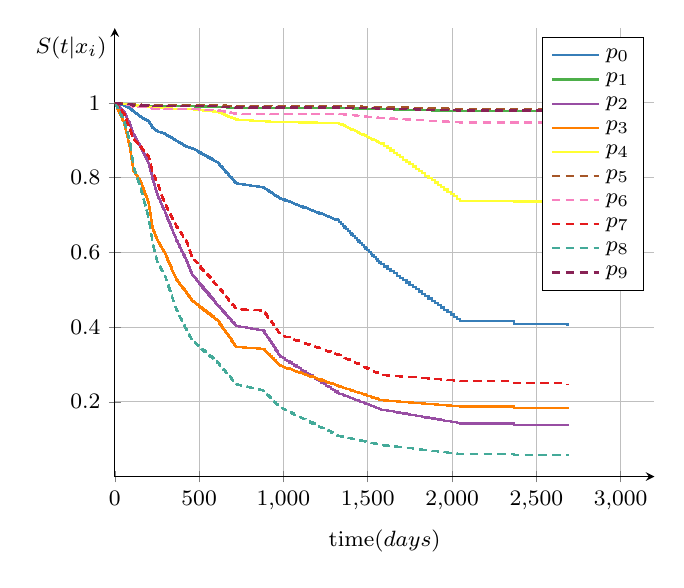
\begin{tikzpicture}[x={(1,0)}]
\footnotesize
\begin{axis}[%
,xlabel=time$(days)$
,ylabel=$S(t|x_i)$
,axis x line = bottom,axis y line = left
,ytick={0.2,0.4,...,1}
,xtick={0,500,1000,...,3000}
,ymax=1.2
,ymin=0
,xmin=0
,xmax=3200
,grid=both
]
%0 
\addplot+[const plot, no marks, thick, c1] coordinates {(0.0, 0.9999852180480957) (2.2, 0.999716579914093) (4.4, 0.9994479417800903) (6.6000000000000005, 0.9991793036460876) (8.8, 0.998910665512085) (11.0, 0.998642086982727) (13.200000000000001, 0.9983734488487244) (15.400000000000002, 0.9981048107147217) (17.6, 0.997836172580719) (19.8, 0.9975675344467163) (22.0, 0.9972988963127136) (24.200000000000003, 0.9970302581787109) (26.400000000000002, 0.9967616200447083) (28.6, 0.9964930415153503) (30.800000000000004, 0.9962244033813477) (33.0, 0.995955765247345) (35.2, 0.9956871271133423) (37.400000000000006, 0.9954184889793396) (39.6, 0.9951498508453369) (41.800000000000004, 0.9948812127113342) (44.0, 0.9946125745773315) (46.2, 0.9943439960479736) (48.400000000000006, 0.994075357913971) (50.6, 0.9938067197799683) (52.800000000000004, 0.9935380816459656) (55.0, 0.9932694435119629) (56.4, 0.9929755926132202) (57.8, 0.9926816821098328) (59.2, 0.9923878312110901) (60.6, 0.9920939803123474) (62.0, 0.99180006980896) (63.4, 0.9915062189102173) (64.8, 0.9912123680114746) (66.2, 0.9909184575080872) (67.6, 0.9906246066093445) (69.0, 0.9903307557106018) (70.4, 0.9900368452072144) (71.8, 0.9897429943084717) (73.2, 0.989449143409729) (74.6, 0.9891552925109863) (76.0, 0.9888613820075989) (77.4, 0.9885675311088562) (78.8, 0.9882736802101135) (80.2, 0.9879797697067261) (81.6, 0.9876859188079834) (83.0, 0.9873920679092407) (84.4, 0.9870981574058533) (85.8, 0.9868043065071106) (87.19999999999999, 0.9865104556083679) (88.6, 0.9862165451049805) (90.0, 0.9859226942062378) (90.8, 0.985596776008606) (91.6, 0.9852709174156189) (92.4, 0.9849449992179871) (93.2, 0.984619140625) (94.0, 0.9842932224273682) (94.8, 0.9839673638343811) (95.6, 0.9836414456367493) (96.4, 0.9833155870437622) (97.2, 0.9829896688461304) (98.0, 0.9826638102531433) (98.8, 0.9823378920555115) (99.6, 0.9820120334625244) (100.4, 0.9816861152648926) (101.2, 0.9813602566719055) (102.0, 0.9810343384742737) (102.8, 0.9807084798812866) (103.6, 0.9803825616836548) (104.4, 0.9800567030906677) (105.2, 0.9797307848930359) (106.0, 0.9794049263000488) (106.8, 0.979079008102417) (107.6, 0.9787531495094299) (108.4, 0.9784272313117981) (109.2, 0.978101372718811) (110.0, 0.9777754545211792) (111.72, 0.9771872162818909) (113.44, 0.9765990376472473) (115.16, 0.976010799407959) (116.88, 0.9754226207733154) (118.6, 0.9748343825340271) (120.32, 0.9742461442947388) (122.03999999999999, 0.9736579656600952) (123.76, 0.9730697274208069) (125.48, 0.9724815487861633) (127.2, 0.971893310546875) (128.92, 0.9713050723075867) (130.64, 0.9707168936729431) (132.36, 0.9701286554336548) (134.07999999999998, 0.9695404767990112) (135.8, 0.9689522385597229) (137.52, 0.9683640003204346) (139.24, 0.967775821685791) (140.96, 0.9671875834465027) (142.68, 0.9665994048118591) (144.4, 0.9660111665725708) (146.12, 0.9654229283332825) (147.84, 0.9648347496986389) (149.56, 0.9642465114593506) (151.28, 0.963658332824707) (153.0, 0.9630700945854187) (154.92, 0.9625561833381653) (156.84, 0.9620422124862671) (158.76, 0.9615283012390137) (160.68, 0.9610143303871155) (162.6, 0.9605004191398621) (164.52, 0.9599864482879639) (166.44, 0.9594725370407104) (168.36, 0.9589585661888123) (170.28, 0.9584446549415588) (172.2, 0.9579306840896606) (174.12, 0.9574167728424072) (176.04, 0.956902801990509) (177.96, 0.9563888907432556) (179.88, 0.9558749198913574) (181.8, 0.955361008644104) (183.72, 0.9548470377922058) (185.64, 0.9543331265449524) (187.56, 0.9538191556930542) (189.48, 0.9533052444458008) (191.4, 0.9527912735939026) (193.32, 0.9522773623466492) (195.24, 0.951763391494751) (197.16, 0.9512494802474976) (199.07999999999998, 0.9507355093955994) (201.0, 0.950221598148346) (201.96, 0.9495610594749451) (202.92, 0.948900580406189) (203.88, 0.9482400417327881) (204.84, 0.947579562664032) (205.8, 0.9469190239906311) (206.76, 0.946258544921875) (207.72, 0.9455980062484741) (208.68, 0.944937527179718) (209.64, 0.9442769885063171) (210.6, 0.943616509437561) (211.56, 0.9429559707641602) (212.52, 0.942295491695404) (213.48, 0.9416349530220032) (214.44, 0.9409744739532471) (215.4, 0.9403139352798462) (216.36, 0.9396534562110901) (217.32, 0.9389929175376892) (218.28, 0.9383324384689331) (219.24, 0.9376718997955322) (220.2, 0.9370114207267761) (221.16, 0.9363508820533752) (222.12, 0.9356904029846191) (223.07999999999998, 0.9350298643112183) (224.04, 0.9343693852424622) (225.0, 0.9337088465690613) (226.12, 0.9333164691925049) (227.24, 0.9329240918159485) (228.36, 0.9325317144393921) (229.48, 0.9321393370628357) (230.6, 0.9317469596862793) (231.72, 0.9313545823097229) (232.84, 0.9309622049331665) (233.96, 0.9305698275566101) (235.08, 0.9301774501800537) (236.2, 0.9297850728034973) (237.32, 0.9293926954269409) (238.44, 0.9290003180503845) (239.56, 0.9286079406738281) (240.68, 0.9282155632972717) (241.8, 0.9278231859207153) (242.92000000000002, 0.9274308085441589) (244.04, 0.9270384311676025) (245.16, 0.9266460537910461) (246.28, 0.9262536764144897) (247.4, 0.9258612990379333) (248.52, 0.925468921661377) (249.64, 0.9250765442848206) (250.76, 0.9246841669082642) (251.88, 0.9242917895317078) (253.0, 0.9238994121551514) (254.6, 0.9236658215522766) (256.2, 0.9234322905540466) (257.8, 0.9231986999511719) (259.4, 0.9229651689529419) (261.0, 0.9227315783500671) (262.6, 0.9224980473518372) (264.2, 0.9222644567489624) (265.8, 0.9220309257507324) (267.4, 0.9217973351478577) (269.0, 0.9215638041496277) (270.6, 0.9213302135467529) (272.2, 0.921096682548523) (273.8, 0.9208630919456482) (275.4, 0.9206295609474182) (277.0, 0.9203959703445435) (278.6, 0.9201624393463135) (280.2, 0.9199288487434387) (281.8, 0.9196953177452087) (283.4, 0.919461727142334) (285.0, 0.919228196144104) (286.6, 0.9189946055412292) (288.2, 0.9187610745429993) (289.8, 0.9185274839401245) (291.4, 0.9182939529418945) (293.0, 0.9180603623390198) (295.84, 0.9173023104667664) (298.68, 0.9165441989898682) (301.52, 0.9157861471176147) (304.36, 0.9150280952453613) (307.2, 0.9142699837684631) (310.04, 0.9135119318962097) (312.88, 0.9127538800239563) (315.72, 0.9119957685470581) (318.56, 0.9112377166748047) (321.4, 0.9104796648025513) (324.24, 0.9097215533256531) (327.08, 0.9089635014533997) (329.92, 0.9082054495811462) (332.76, 0.9074473977088928) (335.6, 0.9066892862319946) (338.44, 0.9059312343597412) (341.28, 0.9051731824874878) (344.12, 0.9044150710105896) (346.96, 0.9036570191383362) (349.8, 0.9028989672660828) (352.64, 0.9021408557891846) (355.48, 0.9013828039169312) (358.32, 0.9006247520446777) (361.15999999999997, 0.8998666405677795) (364.0, 0.8991085886955261) (366.44, 0.8984590172767639) (368.88, 0.8978093862533569) (371.32, 0.8971598148345947) (373.76, 0.8965101838111877) (376.2, 0.8958606123924255) (378.64, 0.8952109813690186) (381.08, 0.8945614099502563) (383.52, 0.8939117789268494) (385.96, 0.8932622075080872) (388.4, 0.8926125764846802) (390.84, 0.891963005065918) (393.28, 0.891313374042511) (395.72, 0.8906638026237488) (398.15999999999997, 0.8900141716003418) (400.6, 0.8893646001815796) (403.04, 0.8887149691581726) (405.48, 0.8880653977394104) (407.92, 0.8874157667160034) (410.36, 0.8867661952972412) (412.8, 0.8861165642738342) (415.24, 0.885466992855072) (417.68, 0.884817361831665) (420.12, 0.8841677904129028) (422.56, 0.8835181593894958) (425.0, 0.8828685879707336) (426.48, 0.8826503753662109) (427.96, 0.8824321627616882) (429.44, 0.8822139501571655) (430.92, 0.8819957375526428) (432.4, 0.8817775249481201) (433.88, 0.8815593123435974) (435.36, 0.8813410997390747) (436.84, 0.881122887134552) (438.32, 0.8809046745300293) (439.8, 0.8806864619255066) (441.28, 0.8804682493209839) (442.76, 0.8802500367164612) (444.24, 0.8800318837165833) (445.72, 0.8798136711120605) (447.2, 0.8795954585075378) (448.68, 0.8793772459030151) (450.16, 0.8791590332984924) (451.64, 0.8789408206939697) (453.12, 0.878722608089447) (454.6, 0.8785043954849243) (456.08, 0.8782861828804016) (457.56, 0.8780679702758789) (459.04, 0.8778497576713562) (460.52, 0.8776315450668335) (462.0, 0.8774133324623108) (467.84, 0.8759564757347107) (473.68, 0.8744996190071106) (479.52, 0.8730428218841553) (485.36, 0.8715859651565552) (491.2, 0.8701291084289551) (497.04, 0.868672251701355) (502.88, 0.8672154545783997) (508.72, 0.8657585978507996) (514.56, 0.8643017411231995) (520.4, 0.8628448843955994) (526.24, 0.861388087272644) (532.08, 0.859931230545044) (537.92, 0.8584743738174438) (543.76, 0.8570175170898438) (549.6, 0.8555607199668884) (555.44, 0.8541038632392883) (561.28, 0.8526470065116882) (567.12, 0.8511901497840881) (572.96, 0.8497333526611328) (578.8, 0.8482764959335327) (584.64, 0.8468196392059326) (590.48, 0.8453627824783325) (596.3199999999999, 0.8439059257507324) (602.16, 0.8424491286277771) (608.0, 0.840992271900177) (612.4, 0.8387444615364075) (616.8, 0.8364965915679932) (621.2, 0.8342487812042236) (625.6, 0.8320009708404541) (630.0, 0.8297531008720398) (634.4, 0.8275052905082703) (638.8, 0.8252574801445007) (643.2, 0.8230096101760864) (647.6, 0.8207617998123169) (652.0, 0.8185139894485474) (656.4, 0.8162661790847778) (660.8, 0.8140183091163635) (665.2, 0.811770498752594) (669.6, 0.8095226287841797) (674.0, 0.8072748184204102) (678.4, 0.8050270080566406) (682.8, 0.8027791976928711) (687.2, 0.8005313277244568) (691.6, 0.7982835173606873) (696.0, 0.7960357069969177) (700.4, 0.7937878370285034) (704.8, 0.7915400266647339) (709.2, 0.7892922163009644) (713.6, 0.78704434633255) (718.0, 0.7847965359687805) (724.48, 0.7843607664108276) (730.96, 0.7839249968528748) (737.44, 0.7834892868995667) (743.92, 0.7830535173416138) (750.4, 0.7826177477836609) (756.88, 0.782181978225708) (763.36, 0.7817462086677551) (769.84, 0.781310498714447) (776.32, 0.7808747291564941) (782.8, 0.7804389595985413) (789.28, 0.7800031900405884) (795.76, 0.7795674204826355) (802.24, 0.7791317105293274) (808.72, 0.7786959409713745) (815.2, 0.7782601714134216) (821.6800000000001, 0.7778244018554688) (828.16, 0.7773886322975159) (834.64, 0.7769529223442078) (841.12, 0.7765171527862549) (847.6, 0.776081383228302) (854.08, 0.7756456136703491) (860.56, 0.7752098441123962) (867.04, 0.7747741341590881) (873.52, 0.7743383646011353) (880.0, 0.7739025950431824) (884.08, 0.772689938545227) (888.16, 0.7714772820472717) (892.24, 0.7702646255493164) (896.32, 0.7690519690513611) (900.4, 0.7678393125534058) (904.48, 0.7666266560554504) (908.56, 0.7654139399528503) (912.64, 0.764201283454895) (916.72, 0.7629886269569397) (920.8, 0.7617759704589844) (924.88, 0.760563313961029) (928.96, 0.7593506574630737) (933.04, 0.7581380009651184) (937.12, 0.7569253444671631) (941.2, 0.7557126879692078) (945.28, 0.7545000314712524) (949.36, 0.7532873749732971) (953.44, 0.7520747184753418) (957.52, 0.7508620023727417) (961.6, 0.7496493458747864) (965.6800000000001, 0.748436689376831) (969.76, 0.7472240328788757) (973.84, 0.7460113763809204) (977.92, 0.7447987198829651) (982.0, 0.7435860633850098) (995.56, 0.7412683963775635) (1009.12, 0.7389507293701172) (1022.68, 0.7366330623626709) (1036.24, 0.7343153953552246) (1049.8, 0.7319977879524231) (1063.36, 0.7296801209449768) (1076.92, 0.7273624539375305) (1090.48, 0.7250447869300842) (1104.04, 0.7227271199226379) (1117.6, 0.7204094529151917) (1131.16, 0.7180917859077454) (1144.72, 0.7157741189002991) (1158.28, 0.7134565114974976) (1171.84, 0.7111388444900513) (1185.4, 0.708821177482605) (1198.96, 0.7065035104751587) (1212.52, 0.7041858434677124) (1226.08, 0.7018681764602661) (1239.6399999999999, 0.6995505094528198) (1253.2, 0.6972328424453735) (1266.76, 0.6949151754379272) (1280.32, 0.6925975680351257) (1293.88, 0.6902799010276794) (1307.44, 0.6879622340202332) (1321.0, 0.6856445670127869) (1331.32, 0.6809491515159607) (1341.64, 0.6762537956237793) (1351.96, 0.6715583801269531) (1362.28, 0.666862964630127) (1372.6, 0.6621675491333008) (1382.92, 0.6574721932411194) (1393.24, 0.6527767777442932) (1403.56, 0.648081362247467) (1413.88, 0.6433860063552856) (1424.2, 0.6386905908584595) (1434.52, 0.6339951753616333) (1444.84, 0.6292997598648071) (1455.16, 0.6246044039726257) (1465.48, 0.6199089884757996) (1475.8, 0.6152135729789734) (1486.12, 0.610518217086792) (1496.44, 0.6058228015899658) (1506.76, 0.6011273860931396) (1517.08, 0.5964319705963135) (1527.4, 0.5917366147041321) (1537.72, 0.5870411992073059) (1548.04, 0.5823457837104797) (1558.3600000000001, 0.5776503682136536) (1568.68, 0.5729550123214722) (1579.0, 0.568259596824646) (1597.76, 0.5621566772460938) (1616.52, 0.5560538172721863) (1635.28, 0.549950897693634) (1654.04, 0.5438480377197266) (1672.8, 0.5377451181411743) (1691.56, 0.5316422581672668) (1710.32, 0.5255393385887146) (1729.08, 0.5194364786148071) (1747.84, 0.5133335590362549) (1766.6, 0.5072306990623474) (1785.3600000000001, 0.5011277794837952) (1804.12, 0.4950249195098877) (1822.88, 0.48892199993133545) (1841.64, 0.482819139957428) (1860.4, 0.47671622037887573) (1879.16, 0.47061336040496826) (1897.92, 0.464510440826416) (1916.68, 0.45840755105018616) (1935.44, 0.4523046612739563) (1954.2, 0.44620177149772644) (1972.96, 0.4400988817214966) (1991.72, 0.4339959919452667) (2010.48, 0.42789310216903687) (2029.24, 0.421790212392807) (2048.0, 0.41568732261657715) (2366.08, 0.4090840518474579) (2684.16, 0.4024807810783386)};
%1 
\addplot+[const plot, no marks, thick, c2] coordinates {(0.0, 1.0000001192092896) (2.2, 0.999868631362915) (4.4, 0.9997371435165405) (6.6000000000000005, 0.9996055960655212) (8.8, 0.9994741082191467) (11.0, 0.9993426203727722) (13.200000000000001, 0.9992111325263977) (15.400000000000002, 0.9990795850753784) (17.6, 0.9989480972290039) (19.8, 0.9988166093826294) (22.0, 0.9986851215362549) (24.200000000000003, 0.9985535740852356) (26.400000000000002, 0.9984220862388611) (28.6, 0.9982905983924866) (30.800000000000004, 0.9981591105461121) (33.0, 0.9980275630950928) (35.2, 0.9978960752487183) (37.400000000000006, 0.9977645874023438) (39.6, 0.9976330995559692) (41.800000000000004, 0.99750155210495) (44.0, 0.9973700642585754) (46.2, 0.9972385764122009) (48.400000000000006, 0.9971070885658264) (50.6, 0.9969755411148071) (52.800000000000004, 0.9968440532684326) (55.0, 0.9967125654220581) (56.4, 0.9967105984687805) (57.8, 0.9967086315155029) (59.2, 0.9967066645622253) (60.6, 0.9967046976089478) (62.0, 0.9967027306556702) (63.4, 0.9967007637023926) (64.8, 0.9966987371444702) (66.2, 0.9966967701911926) (67.6, 0.996694803237915) (69.0, 0.9966928362846375) (70.4, 0.9966908693313599) (71.8, 0.9966889023780823) (73.2, 0.9966869354248047) (74.6, 0.9966849684715271) (76.0, 0.9966830015182495) (77.4, 0.9966810345649719) (78.8, 0.9966790676116943) (80.2, 0.9966771006584167) (81.6, 0.9966750741004944) (83.0, 0.9966731071472168) (84.4, 0.9966711401939392) (85.8, 0.9966691732406616) (87.19999999999999, 0.996667206287384) (88.6, 0.9966652393341064) (90.0, 0.9966632723808289) (90.8, 0.9965046644210815) (91.6, 0.9963459968566895) (92.4, 0.9961873888969421) (93.2, 0.99602872133255) (94.0, 0.9958701133728027) (94.8, 0.9957115054130554) (95.6, 0.9955528378486633) (96.4, 0.995394229888916) (97.2, 0.9952355623245239) (98.0, 0.9950769543647766) (98.8, 0.9949183464050293) (99.6, 0.9947596788406372) (100.4, 0.9946010708808899) (101.2, 0.9944424033164978) (102.0, 0.9942837953567505) (102.8, 0.9941251873970032) (103.6, 0.9939665198326111) (104.4, 0.9938079118728638) (105.2, 0.9936492443084717) (106.0, 0.9934906363487244) (106.8, 0.993332028388977) (107.6, 0.993173360824585) (108.4, 0.9930147528648376) (109.2, 0.9928560853004456) (110.0, 0.9926974773406982) (111.72, 0.9926955103874207) (113.44, 0.9926935434341431) (115.16, 0.9926915168762207) (116.88, 0.9926895499229431) (118.6, 0.9926875829696655) (120.32, 0.9926856160163879) (122.03999999999999, 0.9926836490631104) (123.76, 0.992681622505188) (125.48, 0.9926796555519104) (127.2, 0.9926776885986328) (128.92, 0.9926757216453552) (130.64, 0.9926737546920776) (132.36, 0.9926717281341553) (134.07999999999998, 0.9926697611808777) (135.8, 0.9926677942276001) (137.52, 0.9926658272743225) (139.24, 0.9926638603210449) (140.96, 0.9926618337631226) (142.68, 0.992659866809845) (144.4, 0.9926578998565674) (146.12, 0.9926559329032898) (147.84, 0.9926539659500122) (149.56, 0.9926519393920898) (151.28, 0.9926499724388123) (153.0, 0.9926480054855347) (154.92, 0.9926444292068481) (156.84, 0.9926408529281616) (158.76, 0.9926372766494751) (160.68, 0.9926337003707886) (162.6, 0.992630124092102) (164.52, 0.9926265478134155) (166.44, 0.992622971534729) (168.36, 0.9926193952560425) (170.28, 0.992615818977356) (172.2, 0.9926122426986694) (174.12, 0.9926086664199829) (176.04, 0.9926050901412964) (177.96, 0.9926015734672546) (179.88, 0.9925979971885681) (181.8, 0.9925944209098816) (183.72, 0.9925908446311951) (185.64, 0.9925872683525085) (187.56, 0.992583692073822) (189.48, 0.9925801157951355) (191.4, 0.992576539516449) (193.32, 0.9925729632377625) (195.24, 0.9925693869590759) (197.16, 0.9925658106803894) (199.07999999999998, 0.9925622344017029) (201.0, 0.9925586581230164) (201.96, 0.9924940466880798) (202.92, 0.9924294352531433) (203.88, 0.9923648238182068) (204.84, 0.9923002123832703) (205.8, 0.9922356009483337) (206.76, 0.9921709895133972) (207.72, 0.9921063780784607) (208.68, 0.9920417666435242) (209.64, 0.9919771552085876) (210.6, 0.9919125437736511) (211.56, 0.9918479323387146) (212.52, 0.9917833209037781) (213.48, 0.9917187690734863) (214.44, 0.9916541576385498) (215.4, 0.9915895462036133) (216.36, 0.9915249347686768) (217.32, 0.9914603233337402) (218.28, 0.9913957118988037) (219.24, 0.9913311004638672) (220.2, 0.9912664890289307) (221.16, 0.9912018775939941) (222.12, 0.9911372661590576) (223.07999999999998, 0.9910726547241211) (224.04, 0.9910080432891846) (225.0, 0.990943431854248) (226.12, 0.9909427165985107) (227.24, 0.9909419417381287) (228.36, 0.9909412264823914) (229.48, 0.9909404516220093) (230.6, 0.990939736366272) (231.72, 0.9909389615058899) (232.84, 0.9909382462501526) (233.96, 0.9909374713897705) (235.08, 0.9909367561340332) (236.2, 0.9909359812736511) (237.32, 0.9909352660179138) (238.44, 0.9909344911575317) (239.56, 0.9909337759017944) (240.68, 0.9909330010414124) (241.8, 0.990932285785675) (242.92000000000002, 0.990931510925293) (244.04, 0.9909307956695557) (245.16, 0.9909300208091736) (246.28, 0.9909293055534363) (247.4, 0.9909285306930542) (248.52, 0.9909278154373169) (249.64, 0.9909270405769348) (250.76, 0.9909263253211975) (251.88, 0.9909255504608154) (253.0, 0.9909248352050781) (254.6, 0.9909238219261169) (256.2, 0.9909228086471558) (257.8, 0.9909217953681946) (259.4, 0.9909207820892334) (261.0, 0.990919828414917) (262.6, 0.9909188151359558) (264.2, 0.9909178018569946) (265.8, 0.9909167885780334) (267.4, 0.9909157752990723) (269.0, 0.9909147620201111) (270.6, 0.9909137487411499) (272.2, 0.9909127354621887) (273.8, 0.9909117817878723) (275.4, 0.9909107685089111) (277.0, 0.99090975522995) (278.6, 0.9909087419509888) (280.2, 0.9909077286720276) (281.8, 0.9909067153930664) (283.4, 0.9909057021141052) (285.0, 0.990904688835144) (286.6, 0.9909037351608276) (288.2, 0.9909027218818665) (289.8, 0.9909017086029053) (291.4, 0.9909006953239441) (293.0, 0.9908996820449829) (295.84, 0.9908974766731262) (298.68, 0.9908953309059143) (301.52, 0.9908931255340576) (304.36, 0.9908909797668457) (307.2, 0.990888774394989) (310.04, 0.9908866286277771) (312.88, 0.9908844232559204) (315.72, 0.9908822774887085) (318.56, 0.9908800721168518) (321.4, 0.9908779263496399) (324.24, 0.9908757209777832) (327.08, 0.9908735752105713) (329.92, 0.9908713698387146) (332.76, 0.9908692240715027) (335.6, 0.990867018699646) (338.44, 0.9908648729324341) (341.28, 0.9908626675605774) (344.12, 0.9908605217933655) (346.96, 0.9908583164215088) (349.8, 0.9908561706542969) (352.64, 0.9908539652824402) (355.48, 0.9908518195152283) (358.32, 0.9908496141433716) (361.15999999999997, 0.9908474683761597) (364.0, 0.990845263004303) (366.44, 0.9908443093299866) (368.88, 0.9908434152603149) (371.32, 0.9908424615859985) (373.76, 0.9908415079116821) (376.2, 0.9908405542373657) (378.64, 0.9908396601676941) (381.08, 0.9908387064933777) (383.52, 0.9908377528190613) (385.96, 0.9908368587493896) (388.4, 0.9908359050750732) (390.84, 0.9908349514007568) (393.28, 0.9908339977264404) (395.72, 0.9908331036567688) (398.15999999999997, 0.9908321499824524) (400.6, 0.990831196308136) (403.04, 0.9908302426338196) (405.48, 0.990829348564148) (407.92, 0.9908283948898315) (410.36, 0.9908274412155151) (412.8, 0.9908265471458435) (415.24, 0.9908255934715271) (417.68, 0.9908246397972107) (420.12, 0.9908236861228943) (422.56, 0.9908227920532227) (425.0, 0.9908218383789062) (426.48, 0.9908214211463928) (427.96, 0.9908210635185242) (429.44, 0.9908206462860107) (430.92, 0.9908202886581421) (432.4, 0.9908198714256287) (433.88, 0.99081951379776) (435.36, 0.9908190965652466) (436.84, 0.9908187389373779) (438.32, 0.9908183217048645) (439.8, 0.9908179640769958) (441.28, 0.9908175468444824) (442.76, 0.9908171892166138) (444.24, 0.9908167719841003) (445.72, 0.9908164143562317) (447.2, 0.9908159971237183) (448.68, 0.9908156394958496) (450.16, 0.9908152222633362) (451.64, 0.9908148646354675) (453.12, 0.9908144474029541) (454.6, 0.9908140897750854) (456.08, 0.990813672542572) (457.56, 0.9908133149147034) (459.04, 0.9908128976821899) (460.52, 0.9908125400543213) (462.0, 0.9908121228218079) (467.84, 0.9907740354537964) (473.68, 0.9907359480857849) (479.52, 0.9906978607177734) (485.36, 0.990659773349762) (491.2, 0.9906216859817505) (497.04, 0.990583598613739) (502.88, 0.9905455112457275) (508.72, 0.9905074238777161) (514.56, 0.9904693365097046) (520.4, 0.9904312491416931) (526.24, 0.9903931617736816) (532.08, 0.9903550744056702) (537.92, 0.9903170466423035) (543.76, 0.990278959274292) (549.6, 0.9902408719062805) (555.44, 0.990202784538269) (561.28, 0.9901646971702576) (567.12, 0.9901266098022461) (572.96, 0.9900885224342346) (578.8, 0.9900504350662231) (584.64, 0.9900123476982117) (590.48, 0.9899742603302002) (596.3199999999999, 0.9899361729621887) (602.16, 0.9898980855941772) (608.0, 0.9898599982261658) (612.4, 0.9897229075431824) (616.8, 0.9895857572555542) (621.2, 0.9894486665725708) (625.6, 0.9893115758895874) (630.0, 0.989174485206604) (634.4, 0.9890373349189758) (638.8, 0.9889002442359924) (643.2, 0.988763153553009) (647.6, 0.9886260032653809) (652.0, 0.9884889125823975) (656.4, 0.9883518218994141) (660.8, 0.9882147312164307) (665.2, 0.9880775809288025) (669.6, 0.9879404902458191) (674.0, 0.9878033995628357) (678.4, 0.9876663088798523) (682.8, 0.9875291585922241) (687.2, 0.9873920679092407) (691.6, 0.9872549772262573) (696.0, 0.9871178269386292) (700.4, 0.9869807362556458) (704.8, 0.9868436455726624) (709.2, 0.986706554889679) (713.6, 0.9865694046020508) (718.0, 0.9864323139190674) (724.48, 0.9864292144775391) (730.96, 0.9864261150360107) (737.44, 0.9864230155944824) (743.92, 0.9864199161529541) (750.4, 0.9864168167114258) (756.88, 0.9864137172698975) (763.36, 0.9864105582237244) (769.84, 0.986407458782196) (776.32, 0.9864043593406677) (782.8, 0.9864012598991394) (789.28, 0.9863981604576111) (795.76, 0.9863950610160828) (802.24, 0.9863919615745544) (808.72, 0.9863888621330261) (815.2, 0.9863857626914978) (821.6800000000001, 0.9863826632499695) (828.16, 0.9863795638084412) (834.64, 0.9863764643669128) (841.12, 0.9863733053207397) (847.6, 0.9863702058792114) (854.08, 0.9863671064376831) (860.56, 0.9863640069961548) (867.04, 0.9863609075546265) (873.52, 0.9863578081130981) (880.0, 0.9863547086715698) (884.08, 0.9863540530204773) (888.16, 0.9863533973693848) (892.24, 0.9863526821136475) (896.32, 0.9863520264625549) (900.4, 0.9863513708114624) (904.48, 0.9863507151603699) (908.56, 0.9863500595092773) (912.64, 0.98634934425354) (916.72, 0.9863486886024475) (920.8, 0.986348032951355) (924.88, 0.9863473773002625) (928.96, 0.9863467216491699) (933.04, 0.9863460063934326) (937.12, 0.9863453507423401) (941.2, 0.9863446950912476) (945.28, 0.986344039440155) (949.36, 0.9863433837890625) (953.44, 0.9863426685333252) (957.52, 0.9863420128822327) (961.6, 0.9863413572311401) (965.6800000000001, 0.9863407015800476) (969.76, 0.9863400459289551) (973.84, 0.9863393306732178) (977.92, 0.9863386750221252) (982.0, 0.9863380193710327) (995.56, 0.9863378405570984) (1009.12, 0.9863376617431641) (1022.68, 0.9863374829292297) (1036.24, 0.9863373041152954) (1049.8, 0.9863371849060059) (1063.36, 0.9863370060920715) (1076.92, 0.9863368272781372) (1090.48, 0.9863366484642029) (1104.04, 0.9863364696502686) (1117.6, 0.9863362908363342) (1131.16, 0.9863361120223999) (1144.72, 0.9863359332084656) (1158.28, 0.986335813999176) (1171.84, 0.9863356351852417) (1185.4, 0.9863354563713074) (1198.96, 0.986335277557373) (1212.52, 0.9863350987434387) (1226.08, 0.9863349199295044) (1239.6399999999999, 0.9863347411155701) (1253.2, 0.9863345623016357) (1266.76, 0.9863344430923462) (1280.32, 0.9863342642784119) (1293.88, 0.9863340854644775) (1307.44, 0.9863339066505432) (1321.0, 0.9863337278366089) (1331.32, 0.9862192273139954) (1341.64, 0.9861047863960266) (1351.96, 0.9859902858734131) (1362.28, 0.9858757853507996) (1372.6, 0.9857613444328308) (1382.92, 0.9856468439102173) (1393.24, 0.9855323433876038) (1403.56, 0.985417902469635) (1413.88, 0.9853034019470215) (1424.2, 0.985188901424408) (1434.52, 0.9850744605064392) (1444.84, 0.9849599599838257) (1455.16, 0.9848454594612122) (1465.48, 0.9847309589385986) (1475.8, 0.9846165180206299) (1486.12, 0.9845020174980164) (1496.44, 0.9843875169754028) (1506.76, 0.9842730760574341) (1517.08, 0.9841585755348206) (1527.4, 0.984044075012207) (1537.72, 0.9839296340942383) (1548.04, 0.9838151335716248) (1558.3600000000001, 0.9837006330490112) (1568.68, 0.9835861921310425) (1579.0, 0.983471691608429) (1597.76, 0.9832565784454346) (1616.52, 0.9830414056777954) (1635.28, 0.982826292514801) (1654.04, 0.9826111197471619) (1672.8, 0.9823960065841675) (1691.56, 0.9821808338165283) (1710.32, 0.9819657206535339) (1729.08, 0.9817505478858948) (1747.84, 0.9815354347229004) (1766.6, 0.981320321559906) (1785.3600000000001, 0.9811051487922668) (1804.12, 0.9808900356292725) (1822.88, 0.9806748628616333) (1841.64, 0.9804597496986389) (1860.4, 0.9802445769309998) (1879.16, 0.9800294637680054) (1897.92, 0.979814350605011) (1916.68, 0.9795991778373718) (1935.44, 0.9793840646743774) (1954.2, 0.9791688919067383) (1972.96, 0.9789537787437439) (1991.72, 0.9787386059761047) (2010.48, 0.9785234928131104) (2029.24, 0.9783083200454712) (2048.0, 0.9780932068824768) (2366.08, 0.9780598878860474) (2684.16, 0.9780266284942627)};
%2 
\addplot+[const plot, no marks, thick, c3] coordinates {(0.0, 0.999793529510498) (2.2, 0.9988389015197754) (4.4, 0.9978843331336975) (6.6000000000000005, 0.9969297051429749) (8.8, 0.9959750771522522) (11.0, 0.9950205087661743) (13.200000000000001, 0.9940658807754517) (15.400000000000002, 0.993111252784729) (17.6, 0.9921566843986511) (19.8, 0.9912020564079285) (22.0, 0.9902474284172058) (24.200000000000003, 0.9892928600311279) (26.400000000000002, 0.9883382320404053) (28.6, 0.9873836040496826) (30.800000000000004, 0.98642897605896) (33.0, 0.9854744076728821) (35.2, 0.9845197796821594) (37.400000000000006, 0.9835651516914368) (39.6, 0.9826105833053589) (41.800000000000004, 0.9816559553146362) (44.0, 0.9807013273239136) (46.2, 0.9797467589378357) (48.400000000000006, 0.978792130947113) (50.6, 0.9778375029563904) (52.800000000000004, 0.9768829345703125) (55.0, 0.9759283065795898) (56.4, 0.9746318459510803) (57.8, 0.973335325717926) (59.2, 0.9720388650894165) (60.6, 0.9707423448562622) (62.0, 0.9694458842277527) (63.4, 0.9681493639945984) (64.8, 0.9668529033660889) (66.2, 0.9655563831329346) (67.6, 0.964259922504425) (69.0, 0.9629634618759155) (70.4, 0.9616669416427612) (71.8, 0.9603704810142517) (73.2, 0.9590739607810974) (74.6, 0.9577775001525879) (76.0, 0.9564809799194336) (77.4, 0.9551845192909241) (78.8, 0.9538880586624146) (80.2, 0.9525915384292603) (81.6, 0.9512950778007507) (83.0, 0.9499985575675964) (84.4, 0.9487020969390869) (85.8, 0.9474055767059326) (87.19999999999999, 0.9461091160774231) (88.6, 0.9448125958442688) (90.0, 0.9435161352157593) (90.8, 0.9424722194671631) (91.6, 0.9414282441139221) (92.4, 0.9403843283653259) (93.2, 0.9393404126167297) (94.0, 0.9382964968681335) (94.8, 0.9372525215148926) (95.6, 0.9362086057662964) (96.4, 0.9351646900177002) (97.2, 0.9341207146644592) (98.0, 0.933076798915863) (98.8, 0.9320328831672668) (99.6, 0.9309889674186707) (100.4, 0.9299449920654297) (101.2, 0.9289010763168335) (102.0, 0.9278571605682373) (102.8, 0.9268132448196411) (103.6, 0.9257692694664001) (104.4, 0.924725353717804) (105.2, 0.9236814379692078) (106.0, 0.9226374626159668) (106.8, 0.9215935468673706) (107.6, 0.9205496311187744) (108.4, 0.9195057153701782) (109.2, 0.9184617400169373) (110.0, 0.9174178242683411) (111.72, 0.9160090684890747) (113.44, 0.9146002531051636) (115.16, 0.9131914973258972) (116.88, 0.9117827415466309) (118.6, 0.9103739261627197) (120.32, 0.9089651703834534) (122.03999999999999, 0.907556414604187) (123.76, 0.9061475992202759) (125.48, 0.9047388434410095) (127.2, 0.9033300876617432) (128.92, 0.901921272277832) (130.64, 0.9005125164985657) (132.36, 0.8991037607192993) (134.07999999999998, 0.897695004940033) (135.8, 0.8962861895561218) (137.52, 0.8948774337768555) (139.24, 0.8934686779975891) (140.96, 0.892059862613678) (142.68, 0.8906511068344116) (144.4, 0.8892423510551453) (146.12, 0.8878335356712341) (147.84, 0.8864247798919678) (149.56, 0.8850160241127014) (151.28, 0.8836072087287903) (153.0, 0.8821984529495239) (154.92, 0.8804287314414978) (156.84, 0.8786590695381165) (158.76, 0.8768893480300903) (160.68, 0.875119686126709) (162.6, 0.8733499646186829) (164.52, 0.8715803027153015) (166.44, 0.8698105812072754) (168.36, 0.868040919303894) (170.28, 0.8662711977958679) (172.2, 0.8645015358924866) (174.12, 0.8627318143844604) (176.04, 0.8609621524810791) (177.96, 0.859192430973053) (179.88, 0.8574227690696716) (181.8, 0.8556530475616455) (183.72, 0.8538833856582642) (185.64, 0.852113664150238) (187.56, 0.8503440022468567) (189.48, 0.8485742807388306) (191.4, 0.8468046188354492) (193.32, 0.8450348973274231) (195.24, 0.8432652354240417) (197.16, 0.8414955139160156) (199.07999999999998, 0.8397258520126343) (201.0, 0.8379561305046082) (201.96, 0.8362635970115662) (202.92, 0.8345710039138794) (203.88, 0.8328784704208374) (204.84, 0.8311859369277954) (205.8, 0.8294933438301086) (206.76, 0.8278008103370667) (207.72, 0.8261082172393799) (208.68, 0.8244156837463379) (209.64, 0.8227231502532959) (210.6, 0.8210305571556091) (211.56, 0.8193380236625671) (212.52, 0.8176454901695251) (213.48, 0.8159528970718384) (214.44, 0.8142603635787964) (215.4, 0.8125678300857544) (216.36, 0.8108752369880676) (217.32, 0.8091827034950256) (218.28, 0.8074901103973389) (219.24, 0.8057975769042969) (220.2, 0.8041050434112549) (221.16, 0.8024124503135681) (222.12, 0.8007199168205261) (223.07999999999998, 0.7990273833274841) (224.04, 0.7973347902297974) (225.0, 0.7956422567367554) (226.12, 0.7939435243606567) (227.24, 0.7922447919845581) (228.36, 0.7905460596084595) (229.48, 0.7888473272323608) (230.6, 0.7871485948562622) (231.72, 0.7854498624801636) (232.84, 0.7837511301040649) (233.96, 0.7820523977279663) (235.08, 0.7803536653518677) (236.2, 0.778654932975769) (237.32, 0.7769562005996704) (238.44, 0.7752574682235718) (239.56, 0.7735587954521179) (240.68, 0.7718600630760193) (241.8, 0.7701613306999207) (242.92000000000002, 0.768462598323822) (244.04, 0.7667638659477234) (245.16, 0.7650651335716248) (246.28, 0.7633664011955261) (247.4, 0.7616676688194275) (248.52, 0.7599689364433289) (249.64, 0.7582702040672302) (250.76, 0.7565714716911316) (251.88, 0.754872739315033) (253.0, 0.7531740069389343) (254.6, 0.7515546679496765) (256.2, 0.7499353289604187) (257.8, 0.7483159899711609) (259.4, 0.7466966509819031) (261.0, 0.7450772523880005) (262.6, 0.7434579133987427) (264.2, 0.7418385744094849) (265.8, 0.740219235420227) (267.4, 0.7385998964309692) (269.0, 0.7369805574417114) (270.6, 0.7353612184524536) (272.2, 0.7337418794631958) (273.8, 0.7321224808692932) (275.4, 0.7305031418800354) (277.0, 0.7288838028907776) (278.6, 0.7272644639015198) (280.2, 0.725645124912262) (281.8, 0.7240257859230042) (283.4, 0.7224064469337463) (285.0, 0.7207871079444885) (286.6, 0.7191677093505859) (288.2, 0.7175483703613281) (289.8, 0.7159290313720703) (291.4, 0.7143096923828125) (293.0, 0.7126903533935547) (295.84, 0.7095372080802917) (298.68, 0.7063841223716736) (301.52, 0.7032309770584106) (304.36, 0.7000778913497925) (307.2, 0.6969247460365295) (310.04, 0.6937716603279114) (312.88, 0.6906185150146484) (315.72, 0.6874654293060303) (318.56, 0.6843122839927673) (321.4, 0.6811591386795044) (324.24, 0.6780060529708862) (327.08, 0.6748529076576233) (329.92, 0.6716998219490051) (332.76, 0.6685466766357422) (335.6, 0.665393590927124) (338.44, 0.6622404456138611) (341.28, 0.6590873003005981) (344.12, 0.65593421459198) (346.96, 0.652781069278717) (349.8, 0.6496279835700989) (352.64, 0.6464748382568359) (355.48, 0.6433217525482178) (358.32, 0.6401686072349548) (361.15999999999997, 0.6370155215263367) (364.0, 0.6338623762130737) (366.44, 0.6316288113594055) (368.88, 0.6293953061103821) (371.32, 0.6271617412567139) (373.76, 0.6249282360076904) (376.2, 0.6226946711540222) (378.64, 0.6204611659049988) (381.08, 0.6182276010513306) (383.52, 0.6159940958023071) (385.96, 0.6137605309486389) (388.4, 0.6115270256996155) (390.84, 0.6092934608459473) (393.28, 0.6070599555969238) (395.72, 0.6048263907432556) (398.15999999999997, 0.6025928854942322) (400.6, 0.600359320640564) (403.04, 0.5981258153915405) (405.48, 0.5958922505378723) (407.92, 0.5936587452888489) (410.36, 0.5914251804351807) (412.8, 0.5891916751861572) (415.24, 0.586958110332489) (417.68, 0.5847246050834656) (420.12, 0.5824910402297974) (422.56, 0.5802575349807739) (425.0, 0.5780239701271057) (426.48, 0.5763756632804871) (427.96, 0.5747272968292236) (429.44, 0.573078989982605) (430.92, 0.5714306235313416) (432.4, 0.5697823166847229) (433.88, 0.5681339502334595) (435.36, 0.5664856433868408) (436.84, 0.5648372769355774) (438.32, 0.5631889700889587) (439.8, 0.5615406632423401) (441.28, 0.5598922967910767) (442.76, 0.558243989944458) (444.24, 0.5565956234931946) (445.72, 0.5549473166465759) (447.2, 0.5532989501953125) (448.68, 0.5516506433486938) (450.16, 0.5500023365020752) (451.64, 0.5483539700508118) (453.12, 0.5467056632041931) (454.6, 0.5450572967529297) (456.08, 0.543408989906311) (457.56, 0.5417606234550476) (459.04, 0.540112316608429) (460.52, 0.5384639501571655) (462.0, 0.5368156433105469) (467.84, 0.5337255001068115) (473.68, 0.5306353569030762) (479.52, 0.5275452136993408) (485.36, 0.5244550704956055) (491.2, 0.5213649272918701) (497.04, 0.5182747840881348) (502.88, 0.5151846408843994) (508.72, 0.5120944976806641) (514.56, 0.5090043544769287) (520.4, 0.5059142112731934) (526.24, 0.502824068069458) (532.08, 0.49973389506340027) (537.92, 0.4966437518596649) (543.76, 0.49355360865592957) (549.6, 0.4904634654521942) (555.44, 0.48737332224845886) (561.28, 0.4842831790447235) (567.12, 0.48119300603866577) (572.96, 0.4781028628349304) (578.8, 0.47501271963119507) (584.64, 0.4719225764274597) (590.48, 0.46883243322372437) (596.3199999999999, 0.465742290019989) (602.16, 0.46265214681625366) (608.0, 0.4595620036125183) (612.4, 0.4573078155517578) (616.8, 0.4550536572933197) (621.2, 0.4527994692325592) (625.6, 0.4505453109741211) (630.0, 0.4482911229133606) (634.4, 0.4460369646549225) (638.8, 0.443782776594162) (643.2, 0.4415286183357239) (647.6, 0.4392744302749634) (652.0, 0.43702027201652527) (656.4, 0.43476608395576477) (660.8, 0.43251192569732666) (665.2, 0.43025773763656616) (669.6, 0.42800357937812805) (674.0, 0.42574939131736755) (678.4, 0.42349523305892944) (682.8, 0.42124104499816895) (687.2, 0.41898688673973083) (691.6, 0.41673269867897034) (696.0, 0.4144785404205322) (700.4, 0.41222435235977173) (704.8, 0.4099701941013336) (709.2, 0.4077160060405731) (713.6, 0.405461847782135) (718.0, 0.4032076597213745) (724.48, 0.40271151065826416) (730.96, 0.4022153615951538) (737.44, 0.40171921253204346) (743.92, 0.4012230932712555) (750.4, 0.40072694420814514) (756.88, 0.4002307951450348) (763.36, 0.39973464608192444) (769.84, 0.3992384970188141) (776.32, 0.39874234795570374) (782.8, 0.39824622869491577) (789.28, 0.3977500796318054) (795.76, 0.39725393056869507) (802.24, 0.3967577815055847) (808.72, 0.39626163244247437) (815.2, 0.395765483379364) (821.6800000000001, 0.39526936411857605) (828.16, 0.3947732150554657) (834.64, 0.39427706599235535) (841.12, 0.393780916929245) (847.6, 0.39328476786613464) (854.08, 0.3927886188030243) (860.56, 0.39229249954223633) (867.04, 0.391796350479126) (873.52, 0.3913002014160156) (880.0, 0.3908040523529053) (884.08, 0.38799628615379333) (888.16, 0.3851885497570038) (892.24, 0.38238078355789185) (896.32, 0.3795730173587799) (900.4, 0.37676525115966797) (904.48, 0.3739575147628784) (908.56, 0.3711497485637665) (912.64, 0.36834198236465454) (916.72, 0.365534245967865) (920.8, 0.36272647976875305) (924.88, 0.3599187135696411) (928.96, 0.3571109473705292) (933.04, 0.3543032109737396) (937.12, 0.3514954447746277) (941.2, 0.34868767857551575) (945.28, 0.3458799123764038) (949.36, 0.34307217597961426) (953.44, 0.3402644097805023) (957.52, 0.3374566435813904) (961.6, 0.33464890718460083) (965.6800000000001, 0.3318411409854889) (969.76, 0.32903337478637695) (973.84, 0.3262256383895874) (977.92, 0.32341787219047546) (982.0, 0.3206101059913635) (995.56, 0.31673237681388855) (1009.12, 0.31285467743873596) (1022.68, 0.308976948261261) (1036.24, 0.3050992488861084) (1049.8, 0.3012215197086334) (1063.36, 0.29734379053115845) (1076.92, 0.29346609115600586) (1090.48, 0.2895883619785309) (1104.04, 0.2857106626033783) (1117.6, 0.2818329334259033) (1131.16, 0.27795523405075073) (1144.72, 0.27407750487327576) (1158.28, 0.2701997756958008) (1171.84, 0.2663220763206482) (1185.4, 0.2624443471431732) (1198.96, 0.25856661796569824) (1212.52, 0.25468891859054565) (1226.08, 0.2508111894130707) (1239.6399999999999, 0.2469334751367569) (1253.2, 0.24305576086044312) (1266.76, 0.23917803168296814) (1280.32, 0.23530033230781555) (1293.88, 0.23142260313034058) (1307.44, 0.227544903755188) (1321.0, 0.223667174577713) (1331.32, 0.22188030183315277) (1341.64, 0.22009342908859253) (1351.96, 0.2183065563440323) (1362.28, 0.21651968359947205) (1372.6, 0.214732825756073) (1382.92, 0.21294595301151276) (1393.24, 0.21115908026695251) (1403.56, 0.20937220752239227) (1413.88, 0.20758533477783203) (1424.2, 0.2057984620332718) (1434.52, 0.20401158928871155) (1444.84, 0.2022247314453125) (1455.16, 0.20043785870075226) (1465.48, 0.19865098595619202) (1475.8, 0.19686411321163177) (1486.12, 0.19507724046707153) (1496.44, 0.1932903677225113) (1506.76, 0.19150349497795105) (1517.08, 0.1897166222333908) (1527.4, 0.18792974948883057) (1537.72, 0.18614289164543152) (1548.04, 0.18435601890087128) (1558.3600000000001, 0.18256914615631104) (1568.68, 0.1807822734117508) (1579.0, 0.17899540066719055) (1597.76, 0.17751823365688324) (1616.52, 0.17604108154773712) (1635.28, 0.1745639145374298) (1654.04, 0.1730867624282837) (1672.8, 0.17160959541797638) (1691.56, 0.17013244330883026) (1710.32, 0.16865527629852295) (1729.08, 0.16717812418937683) (1747.84, 0.16570095717906952) (1766.6, 0.1642238050699234) (1785.3600000000001, 0.1627466380596161) (1804.12, 0.16126948595046997) (1822.88, 0.15979231894016266) (1841.64, 0.15831516683101654) (1860.4, 0.15683799982070923) (1879.16, 0.1553608477115631) (1897.92, 0.1538836807012558) (1916.68, 0.15240652859210968) (1935.44, 0.15092936158180237) (1954.2, 0.14945220947265625) (1972.96, 0.14797504246234894) (1991.72, 0.14649787545204163) (2010.48, 0.1450207233428955) (2029.24, 0.1435435712337494) (2048.0, 0.14206640422344208) (2366.08, 0.1386365294456482) (2684.16, 0.1352066546678543)};
%3 
\addplot+[const plot, no marks, thick, c4] coordinates {(0.0, 0.9995284080505371) (2.2, 0.9974343776702881) (4.4, 0.9953404068946838) (6.6000000000000005, 0.9932463765144348) (8.8, 0.9911524057388306) (11.0, 0.9890583753585815) (13.200000000000001, 0.9869644045829773) (15.400000000000002, 0.9848703742027283) (17.6, 0.982776403427124) (19.8, 0.980682373046875) (22.0, 0.9785884022712708) (24.200000000000003, 0.9764943718910217) (26.400000000000002, 0.9744004011154175) (28.6, 0.9723063707351685) (30.800000000000004, 0.9702123999595642) (33.0, 0.9681183695793152) (35.2, 0.9660243988037109) (37.400000000000006, 0.9639303684234619) (39.6, 0.9618363976478577) (41.800000000000004, 0.9597423672676086) (44.0, 0.9576483964920044) (46.2, 0.9555543661117554) (48.400000000000006, 0.9534603953361511) (50.6, 0.9513663649559021) (52.800000000000004, 0.9492723941802979) (55.0, 0.9471783638000488) (56.4, 0.9444419741630554) (57.8, 0.9417056441307068) (59.2, 0.9389692544937134) (60.6, 0.93623286485672) (62.0, 0.9334965348243713) (63.4, 0.9307601451873779) (64.8, 0.9280238151550293) (66.2, 0.9252874255180359) (67.6, 0.9225510358810425) (69.0, 0.9198147058486938) (70.4, 0.9170783162117004) (71.8, 0.914341926574707) (73.2, 0.9116055965423584) (74.6, 0.908869206905365) (76.0, 0.9061328172683716) (77.4, 0.903396487236023) (78.8, 0.9006600975990295) (80.2, 0.8979237079620361) (81.6, 0.8951873779296875) (83.0, 0.8924509882926941) (84.4, 0.8897145986557007) (85.8, 0.886978268623352) (87.19999999999999, 0.8842418789863586) (88.6, 0.88150554895401) (90.0, 0.8787691593170166) (90.8, 0.8763835430145264) (91.6, 0.8739979863166809) (92.4, 0.8716123700141907) (93.2, 0.8692267537117004) (94.0, 0.866841197013855) (94.8, 0.8644555807113647) (95.6, 0.8620699644088745) (96.4, 0.859684407711029) (97.2, 0.8572987914085388) (98.0, 0.8549131751060486) (98.8, 0.8525276184082031) (99.6, 0.8501420021057129) (100.4, 0.8477563858032227) (101.2, 0.8453707695007324) (102.0, 0.842985212802887) (102.8, 0.8405995965003967) (103.6, 0.8382139801979065) (104.4, 0.835828423500061) (105.2, 0.8334428071975708) (106.0, 0.8310571908950806) (106.8, 0.8286716341972351) (107.6, 0.8262860178947449) (108.4, 0.8239004015922546) (109.2, 0.8215148448944092) (110.0, 0.819129228591919) (111.72, 0.8179692625999451) (113.44, 0.816809356212616) (115.16, 0.8156493902206421) (116.88, 0.8144894242286682) (118.6, 0.8133295178413391) (120.32, 0.8121695518493652) (122.03999999999999, 0.8110095858573914) (123.76, 0.8098496794700623) (125.48, 0.8086897134780884) (127.2, 0.8075297474861145) (128.92, 0.8063698410987854) (130.64, 0.8052098751068115) (132.36, 0.8040499091148376) (134.07999999999998, 0.8028899431228638) (135.8, 0.8017300367355347) (137.52, 0.8005700707435608) (139.24, 0.7994101047515869) (140.96, 0.7982501983642578) (142.68, 0.7970902323722839) (144.4, 0.7959302663803101) (146.12, 0.794770359992981) (147.84, 0.7936103940010071) (149.56, 0.7924504280090332) (151.28, 0.7912905216217041) (153.0, 0.7901305556297302) (154.92, 0.7877728343009949) (156.84, 0.7854151129722595) (158.76, 0.783057451248169) (160.68, 0.7806997299194336) (162.6, 0.7783420085906982) (164.52, 0.7759842872619629) (166.44, 0.7736265659332275) (168.36, 0.771268904209137) (170.28, 0.7689111828804016) (172.2, 0.7665534615516663) (174.12, 0.7641957402229309) (176.04, 0.7618380188941956) (177.96, 0.759480357170105) (179.88, 0.7571226358413696) (181.8, 0.7547649145126343) (183.72, 0.7524071931838989) (185.64, 0.7500494718551636) (187.56, 0.747691810131073) (189.48, 0.7453340888023376) (191.4, 0.7429763674736023) (193.32, 0.7406186461448669) (195.24, 0.7382609248161316) (197.16, 0.735903263092041) (199.07999999999998, 0.7335455417633057) (201.0, 0.7311878204345703) (201.96, 0.7284696102142334) (202.92, 0.7257513999938965) (203.88, 0.7230331897735596) (204.84, 0.7203149795532227) (205.8, 0.717596709728241) (206.76, 0.714878499507904) (207.72, 0.7121602892875671) (208.68, 0.7094420790672302) (209.64, 0.7067238688468933) (210.6, 0.7040056586265564) (211.56, 0.7012874484062195) (212.52, 0.6985692381858826) (213.48, 0.6958509683609009) (214.44, 0.693132758140564) (215.4, 0.690414547920227) (216.36, 0.6876963376998901) (217.32, 0.6849781274795532) (218.28, 0.6822599172592163) (219.24, 0.6795417070388794) (220.2, 0.6768234968185425) (221.16, 0.6741052269935608) (222.12, 0.6713870167732239) (223.07999999999998, 0.668668806552887) (224.04, 0.66595059633255) (225.0, 0.6632323861122131) (226.12, 0.6619911193847656) (227.24, 0.6607498526573181) (228.36, 0.6595085859298706) (229.48, 0.6582673192024231) (230.6, 0.6570260524749756) (231.72, 0.6557847857475281) (232.84, 0.6545434594154358) (233.96, 0.6533021926879883) (235.08, 0.6520609259605408) (236.2, 0.6508196592330933) (237.32, 0.6495783925056458) (238.44, 0.6483371257781982) (239.56, 0.6470958590507507) (240.68, 0.6458545923233032) (241.8, 0.6446133255958557) (242.92000000000002, 0.6433720588684082) (244.04, 0.6421307921409607) (245.16, 0.6408895254135132) (246.28, 0.6396481990814209) (247.4, 0.6384069323539734) (248.52, 0.6371656656265259) (249.64, 0.6359243988990784) (250.76, 0.6346831321716309) (251.88, 0.6334418654441833) (253.0, 0.6322005987167358) (254.6, 0.6309685707092285) (256.2, 0.6297364830970764) (257.8, 0.6285044550895691) (259.4, 0.627272367477417) (261.0, 0.6260403394699097) (262.6, 0.6248082518577576) (264.2, 0.6235762238502502) (265.8, 0.6223441362380981) (267.4, 0.6211121082305908) (269.0, 0.6198800206184387) (270.6, 0.6186479926109314) (272.2, 0.6174159049987793) (273.8, 0.616183876991272) (275.4, 0.6149517893791199) (277.0, 0.6137197613716125) (278.6, 0.6124876737594604) (280.2, 0.6112556457519531) (281.8, 0.610023558139801) (283.4, 0.6087915301322937) (285.0, 0.6075594425201416) (286.6, 0.6063274145126343) (288.2, 0.6050953269004822) (289.8, 0.6038632988929749) (291.4, 0.6026312112808228) (293.0, 0.6013991832733154) (295.84, 0.5984386801719666) (298.68, 0.5954781770706177) (301.52, 0.5925177335739136) (304.36, 0.5895572304725647) (307.2, 0.5865967273712158) (310.04, 0.5836362242698669) (312.88, 0.5806757211685181) (315.72, 0.577715277671814) (318.56, 0.5747547745704651) (321.4, 0.5717942714691162) (324.24, 0.5688337683677673) (327.08, 0.5658732652664185) (329.92, 0.5629128217697144) (332.76, 0.5599523186683655) (335.6, 0.5569918155670166) (338.44, 0.5540313124656677) (341.28, 0.5510708093643188) (344.12, 0.5481103658676147) (346.96, 0.5451498627662659) (349.8, 0.542189359664917) (352.64, 0.5392288565635681) (355.48, 0.5362683534622192) (358.32, 0.5333079099655151) (361.15999999999997, 0.5303474068641663) (364.0, 0.5273869037628174) (366.44, 0.5259767174720764) (368.88, 0.5245664715766907) (371.32, 0.5231562852859497) (373.76, 0.5217460989952087) (376.2, 0.5203359127044678) (378.64, 0.518925666809082) (381.08, 0.5175154805183411) (383.52, 0.5161052942276001) (385.96, 0.5146950483322144) (388.4, 0.5132848620414734) (390.84, 0.5118746757507324) (393.28, 0.5104644298553467) (395.72, 0.5090542435646057) (398.15999999999997, 0.5076440572738647) (400.6, 0.506233811378479) (403.04, 0.504823625087738) (405.48, 0.5034134387969971) (407.92, 0.5020032525062561) (410.36, 0.5005930066108704) (412.8, 0.4991828203201294) (415.24, 0.49777260422706604) (417.68, 0.4963624179363251) (420.12, 0.4949522018432617) (422.56, 0.49354201555252075) (425.0, 0.4921317994594574) (426.48, 0.49119314551353455) (427.96, 0.4902545213699341) (429.44, 0.48931586742401123) (430.92, 0.4883772134780884) (432.4, 0.4874385595321655) (433.88, 0.48649993538856506) (435.36, 0.4855612814426422) (436.84, 0.48462262749671936) (438.32, 0.4836840033531189) (439.8, 0.48274534940719604) (441.28, 0.4818066954612732) (442.76, 0.48086804151535034) (444.24, 0.4799294173717499) (445.72, 0.478990763425827) (447.2, 0.4780521094799042) (448.68, 0.4771134853363037) (450.16, 0.47617483139038086) (451.64, 0.475236177444458) (453.12, 0.47429752349853516) (454.6, 0.4733588993549347) (456.08, 0.47242024540901184) (457.56, 0.471481591463089) (459.04, 0.47054293751716614) (460.52, 0.4696043133735657) (462.0, 0.4686656594276428) (467.84, 0.46665826439857483) (473.68, 0.4646508991718292) (479.52, 0.46264350414276123) (485.36, 0.46063610911369324) (491.2, 0.45862874388694763) (497.04, 0.45662134885787964) (502.88, 0.45461398363113403) (508.72, 0.45260658860206604) (514.56, 0.45059919357299805) (520.4, 0.44859182834625244) (526.24, 0.44658443331718445) (532.08, 0.44457703828811646) (537.92, 0.44256967306137085) (543.76, 0.44056227803230286) (549.6, 0.43855488300323486) (555.44, 0.43654751777648926) (561.28, 0.43454012274742126) (567.12, 0.43253272771835327) (572.96, 0.43052536249160767) (578.8, 0.4285179674625397) (584.64, 0.4265105724334717) (590.48, 0.4245032072067261) (596.3199999999999, 0.4224958121776581) (602.16, 0.4204884469509125) (608.0, 0.4184810519218445) (612.4, 0.41562163829803467) (616.8, 0.41276222467422485) (621.2, 0.40990281105041504) (625.6, 0.4070433974266052) (630.0, 0.4041839838027954) (634.4, 0.4013245701789856) (638.8, 0.3984651565551758) (643.2, 0.39560574293136597) (647.6, 0.39274632930755615) (652.0, 0.38988691568374634) (656.4, 0.3870275020599365) (660.8, 0.3841680884361267) (665.2, 0.3813086748123169) (669.6, 0.3784492313861847) (674.0, 0.3755898177623749) (678.4, 0.37273040413856506) (682.8, 0.36987099051475525) (687.2, 0.36701157689094543) (691.6, 0.3641521632671356) (696.0, 0.3612927496433258) (700.4, 0.358433336019516) (704.8, 0.3555739223957062) (709.2, 0.35271450877189636) (713.6, 0.34985509514808655) (718.0, 0.34699568152427673) (724.48, 0.3467830717563629) (730.96, 0.3465704619884491) (737.44, 0.3463578522205353) (743.92, 0.3461452126502991) (750.4, 0.34593260288238525) (756.88, 0.34571999311447144) (763.36, 0.3455073833465576) (769.84, 0.3452947735786438) (776.32, 0.34508216381073) (782.8, 0.3448695242404938) (789.28, 0.34465691447257996) (795.76, 0.34444430470466614) (802.24, 0.3442316949367523) (808.72, 0.3440190851688385) (815.2, 0.3438064754009247) (821.6800000000001, 0.3435938358306885) (828.16, 0.34338122606277466) (834.64, 0.34316861629486084) (841.12, 0.342956006526947) (847.6, 0.3427433967590332) (854.08, 0.3425307869911194) (860.56, 0.3423181474208832) (867.04, 0.34210553765296936) (873.52, 0.34189292788505554) (880.0, 0.3416803181171417) (884.08, 0.33983680605888367) (888.16, 0.3379932940006256) (892.24, 0.33614975214004517) (896.32, 0.3343062400817871) (900.4, 0.33246272802352905) (904.48, 0.330619215965271) (908.56, 0.32877567410469055) (912.64, 0.3269321620464325) (916.72, 0.32508864998817444) (920.8, 0.3232451379299164) (924.88, 0.32140159606933594) (928.96, 0.3195580840110779) (933.04, 0.3177145719528198) (937.12, 0.31587105989456177) (941.2, 0.3140275180339813) (945.28, 0.31218400597572327) (949.36, 0.3103404939174652) (953.44, 0.30849698185920715) (957.52, 0.3066534399986267) (961.6, 0.30480992794036865) (965.6800000000001, 0.3029664158821106) (969.76, 0.30112290382385254) (973.84, 0.2992793917655945) (977.92, 0.29743584990501404) (982.0, 0.295592337846756) (995.56, 0.2934684753417969) (1009.12, 0.29134461283683777) (1022.68, 0.28922075033187866) (1036.24, 0.28709688782691956) (1049.8, 0.28497302532196045) (1063.36, 0.28284916281700134) (1076.92, 0.28072530031204224) (1090.48, 0.27860143780708313) (1104.04, 0.276477575302124) (1117.6, 0.2743537127971649) (1131.16, 0.2722298502922058) (1144.72, 0.2701059877872467) (1158.28, 0.2679821252822876) (1171.84, 0.2658582627773285) (1185.4, 0.2637344002723694) (1198.96, 0.2616105377674103) (1212.52, 0.25948667526245117) (1226.08, 0.25736281275749207) (1239.6399999999999, 0.25523895025253296) (1253.2, 0.25311508774757385) (1266.76, 0.25099122524261475) (1280.32, 0.24886737763881683) (1293.88, 0.24674351513385773) (1307.44, 0.24461965262889862) (1321.0, 0.24249579012393951) (1331.32, 0.24096395075321198) (1341.64, 0.23943211138248444) (1351.96, 0.2379002720117569) (1362.28, 0.23636843264102936) (1372.6, 0.23483659327030182) (1382.92, 0.23330476880073547) (1393.24, 0.23177292943000793) (1403.56, 0.2302410900592804) (1413.88, 0.22870925068855286) (1424.2, 0.22717741131782532) (1434.52, 0.22564557194709778) (1444.84, 0.22411373257637024) (1455.16, 0.2225818932056427) (1465.48, 0.22105005383491516) (1475.8, 0.21951821446418762) (1486.12, 0.21798637509346008) (1496.44, 0.21645453572273254) (1506.76, 0.214922696352005) (1517.08, 0.21339085698127747) (1527.4, 0.21185903251171112) (1537.72, 0.2103271782398224) (1548.04, 0.20879535377025604) (1558.3600000000001, 0.2072635143995285) (1568.68, 0.20573167502880096) (1579.0, 0.20419983565807343) (1597.76, 0.20352597534656525) (1616.52, 0.20285212993621826) (1635.28, 0.20217826962471008) (1654.04, 0.2015044242143631) (1672.8, 0.20083056390285492) (1691.56, 0.20015671849250793) (1710.32, 0.19948285818099976) (1729.08, 0.19880901277065277) (1747.84, 0.1981351524591446) (1766.6, 0.1974613070487976) (1785.3600000000001, 0.19678744673728943) (1804.12, 0.19611360132694244) (1822.88, 0.19543974101543427) (1841.64, 0.19476589560508728) (1860.4, 0.1940920352935791) (1879.16, 0.19341818988323212) (1897.92, 0.19274432957172394) (1916.68, 0.19207048416137695) (1935.44, 0.19139662384986877) (1954.2, 0.1907227784395218) (1972.96, 0.1900489181280136) (1991.72, 0.18937507271766663) (2010.48, 0.18870121240615845) (2029.24, 0.18802735209465027) (2048.0, 0.18735350668430328) (2366.08, 0.18445686995983124) (2684.16, 0.18156024813652039)};
%4 
\addplot+[const plot, no marks, thick, c5] coordinates {(0.0, 0.9999998211860657) (2.2, 0.9999100565910339) (4.4, 0.9998202919960022) (6.6000000000000005, 0.9997304677963257) (8.8, 0.999640703201294) (11.0, 0.9995509386062622) (13.200000000000001, 0.9994611740112305) (15.400000000000002, 0.999371349811554) (17.6, 0.9992815852165222) (19.8, 0.9991918206214905) (22.0, 0.9991020560264587) (24.200000000000003, 0.9990122318267822) (26.400000000000002, 0.9989224672317505) (28.6, 0.9988327026367188) (30.800000000000004, 0.998742938041687) (33.0, 0.9986531138420105) (35.2, 0.9985633492469788) (37.400000000000006, 0.998473584651947) (39.6, 0.9983838200569153) (41.800000000000004, 0.9982939958572388) (44.0, 0.998204231262207) (46.2, 0.9981144666671753) (48.400000000000006, 0.9980247020721436) (50.6, 0.997934877872467) (52.800000000000004, 0.9978451132774353) (55.0, 0.9977553486824036) (56.4, 0.9977306127548218) (57.8, 0.99770587682724) (59.2, 0.9976810812950134) (60.6, 0.9976563453674316) (62.0, 0.9976316094398499) (63.4, 0.9976068735122681) (64.8, 0.9975821375846863) (66.2, 0.9975573420524597) (67.6, 0.9975326061248779) (69.0, 0.9975078701972961) (70.4, 0.9974831342697144) (71.8, 0.9974583983421326) (73.2, 0.997433602809906) (74.6, 0.9974088668823242) (76.0, 0.9973841309547424) (77.4, 0.9973593950271606) (78.8, 0.9973346590995789) (80.2, 0.9973098635673523) (81.6, 0.9972851276397705) (83.0, 0.9972603917121887) (84.4, 0.9972356557846069) (85.8, 0.9972109198570251) (87.19999999999999, 0.9971861243247986) (88.6, 0.9971613883972168) (90.0, 0.997136652469635) (90.8, 0.9970266222953796) (91.6, 0.9969165325164795) (92.4, 0.9968065023422241) (93.2, 0.9966964721679688) (94.0, 0.9965863823890686) (94.8, 0.9964763522148132) (95.6, 0.9963663220405579) (96.4, 0.9962562322616577) (97.2, 0.9961462020874023) (98.0, 0.996036171913147) (98.8, 0.9959260821342468) (99.6, 0.9958160519599915) (100.4, 0.9957060217857361) (101.2, 0.9955959916114807) (102.0, 0.9954859018325806) (102.8, 0.9953758716583252) (103.6, 0.9952658414840698) (104.4, 0.9951557517051697) (105.2, 0.9950457215309143) (106.0, 0.9949356913566589) (106.8, 0.9948256015777588) (107.6, 0.9947155714035034) (108.4, 0.994605541229248) (109.2, 0.9944954514503479) (110.0, 0.9943854212760925) (111.72, 0.994271457195282) (113.44, 0.9941574931144714) (115.16, 0.9940435886383057) (116.88, 0.9939296245574951) (118.6, 0.9938156604766846) (120.32, 0.993701696395874) (122.03999999999999, 0.9935877919197083) (123.76, 0.9934738278388977) (125.48, 0.9933598637580872) (127.2, 0.9932458996772766) (128.92, 0.9931319952011108) (130.64, 0.9930180311203003) (132.36, 0.9929040670394897) (134.07999999999998, 0.9927901029586792) (135.8, 0.9926761984825134) (137.52, 0.9925622344017029) (139.24, 0.9924482703208923) (140.96, 0.9923343062400818) (142.68, 0.992220401763916) (144.4, 0.9921064376831055) (146.12, 0.9919924736022949) (147.84, 0.9918785095214844) (149.56, 0.9917646050453186) (151.28, 0.9916506409645081) (153.0, 0.9915366768836975) (154.92, 0.9914776682853699) (156.84, 0.9914186596870422) (158.76, 0.9913597106933594) (160.68, 0.9913007020950317) (162.6, 0.9912416934967041) (164.52, 0.9911826848983765) (166.44, 0.9911236763000488) (168.36, 0.991064727306366) (170.28, 0.9910057187080383) (172.2, 0.9909467101097107) (174.12, 0.9908877015113831) (176.04, 0.9908286929130554) (177.96, 0.9907697439193726) (179.88, 0.9907107353210449) (181.8, 0.9906517267227173) (183.72, 0.9905927181243896) (185.64, 0.990533709526062) (187.56, 0.9904747605323792) (189.48, 0.9904157519340515) (191.4, 0.9903567433357239) (193.32, 0.9902977347373962) (195.24, 0.9902387261390686) (197.16, 0.9901797771453857) (199.07999999999998, 0.9901207685470581) (201.0, 0.9900617599487305) (201.96, 0.9899367690086365) (202.92, 0.9898117780685425) (203.88, 0.9896867871284485) (204.84, 0.9895617961883545) (205.8, 0.9894368648529053) (206.76, 0.9893118739128113) (207.72, 0.9891868829727173) (208.68, 0.9890618920326233) (209.64, 0.9889369010925293) (210.6, 0.9888119101524353) (211.56, 0.9886869192123413) (212.52, 0.9885619282722473) (213.48, 0.9884369969367981) (214.44, 0.9883120059967041) (215.4, 0.9881870150566101) (216.36, 0.9880620241165161) (217.32, 0.9879370331764221) (218.28, 0.9878120422363281) (219.24, 0.9876870512962341) (220.2, 0.9875620603561401) (221.16, 0.9874371290206909) (222.12, 0.9873121380805969) (223.07999999999998, 0.9871871471405029) (224.04, 0.9870621562004089) (225.0, 0.9869371652603149) (226.12, 0.9869015216827393) (227.24, 0.9868658185005188) (228.36, 0.9868301749229431) (229.48, 0.9867945313453674) (230.6, 0.9867588877677917) (231.72, 0.9867231845855713) (232.84, 0.9866875410079956) (233.96, 0.9866518974304199) (235.08, 0.9866161942481995) (236.2, 0.9865805506706238) (237.32, 0.9865449070930481) (238.44, 0.9865092635154724) (239.56, 0.986473560333252) (240.68, 0.9864379167556763) (241.8, 0.9864022731781006) (242.92000000000002, 0.9863666296005249) (244.04, 0.9863309264183044) (245.16, 0.9862952828407288) (246.28, 0.9862596392631531) (247.4, 0.9862239360809326) (248.52, 0.9861882925033569) (249.64, 0.9861526489257812) (250.76, 0.9861170053482056) (251.88, 0.9860813021659851) (253.0, 0.9860456585884094) (254.6, 0.9860256910324097) (256.2, 0.9860057830810547) (257.8, 0.9859858155250549) (259.4, 0.9859658479690552) (261.0, 0.9859459400177002) (262.6, 0.9859259724617004) (264.2, 0.9859060049057007) (265.8, 0.9858860969543457) (267.4, 0.985866129398346) (269.0, 0.9858461618423462) (270.6, 0.9858262538909912) (272.2, 0.9858062863349915) (273.8, 0.9857863187789917) (275.4, 0.9857663512229919) (277.0, 0.985746443271637) (278.6, 0.9857264757156372) (280.2, 0.9857065081596375) (281.8, 0.9856866002082825) (283.4, 0.9856666326522827) (285.0, 0.985646665096283) (286.6, 0.985626757144928) (288.2, 0.9856067895889282) (289.8, 0.9855868220329285) (291.4, 0.9855669140815735) (293.0, 0.9855469465255737) (295.84, 0.9855015277862549) (298.68, 0.985456109046936) (301.52, 0.985410749912262) (304.36, 0.9853653311729431) (307.2, 0.9853199124336243) (310.04, 0.9852744936943054) (312.88, 0.9852290749549866) (315.72, 0.9851837158203125) (318.56, 0.9851382970809937) (321.4, 0.9850928783416748) (324.24, 0.985047459602356) (327.08, 0.9850020408630371) (329.92, 0.984956681728363) (332.76, 0.9849112629890442) (335.6, 0.9848658442497253) (338.44, 0.9848204255104065) (341.28, 0.9847750067710876) (344.12, 0.9847296476364136) (346.96, 0.9846842288970947) (349.8, 0.9846388101577759) (352.64, 0.984593391418457) (355.48, 0.9845479726791382) (358.32, 0.9845026135444641) (361.15999999999997, 0.9844571948051453) (364.0, 0.9844117760658264) (366.44, 0.9843619465827942) (368.88, 0.984312117099762) (371.32, 0.9842623472213745) (373.76, 0.9842125177383423) (376.2, 0.9841626882553101) (378.64, 0.9841128587722778) (381.08, 0.9840630888938904) (383.52, 0.9840132594108582) (385.96, 0.9839634299278259) (388.4, 0.9839136004447937) (390.84, 0.9838638305664062) (393.28, 0.983814001083374) (395.72, 0.9837641716003418) (398.15999999999997, 0.9837143421173096) (400.6, 0.9836645722389221) (403.04, 0.9836147427558899) (405.48, 0.9835649132728577) (407.92, 0.9835150837898254) (410.36, 0.983465313911438) (412.8, 0.9834154844284058) (415.24, 0.9833656549453735) (417.68, 0.9833158254623413) (420.12, 0.9832660555839539) (422.56, 0.9832162261009216) (425.0, 0.9831663966178894) (426.48, 0.9831506013870239) (427.96, 0.9831348061561584) (429.44, 0.9831190705299377) (430.92, 0.9831032752990723) (432.4, 0.9830874800682068) (433.88, 0.9830716848373413) (435.36, 0.9830558896064758) (436.84, 0.9830401539802551) (438.32, 0.9830243587493896) (439.8, 0.9830085635185242) (441.28, 0.9829927682876587) (442.76, 0.9829769730567932) (444.24, 0.9829612374305725) (445.72, 0.982945442199707) (447.2, 0.9829296469688416) (448.68, 0.9829138517379761) (450.16, 0.9828980565071106) (451.64, 0.9828823208808899) (453.12, 0.9828665256500244) (454.6, 0.9828507304191589) (456.08, 0.9828349351882935) (457.56, 0.982819139957428) (459.04, 0.9828034043312073) (460.52, 0.9827876091003418) (462.0, 0.9827718138694763) (467.84, 0.982511579990387) (473.68, 0.9822513461112976) (479.52, 0.981991171836853) (485.36, 0.9817309379577637) (491.2, 0.9814707040786743) (497.04, 0.981210470199585) (502.88, 0.9809502363204956) (508.72, 0.980690062046051) (514.56, 0.9804298281669617) (520.4, 0.9801695942878723) (526.24, 0.979909360408783) (532.08, 0.9796491265296936) (537.92, 0.979388952255249) (543.76, 0.9791287183761597) (549.6, 0.9788684844970703) (555.44, 0.978608250617981) (561.28, 0.9783480167388916) (567.12, 0.978087842464447) (572.96, 0.9778276085853577) (578.8, 0.9775673747062683) (584.64, 0.977307140827179) (590.48, 0.9770469069480896) (596.3199999999999, 0.976786732673645) (602.16, 0.9765264987945557) (608.0, 0.9762662649154663) (612.4, 0.9754424095153809) (616.8, 0.9746185541152954) (621.2, 0.97379469871521) (625.6, 0.9729708433151245) (630.0, 0.9721469879150391) (634.4, 0.9713231325149536) (638.8, 0.9704992771148682) (643.2, 0.9696754217147827) (647.6, 0.9688515663146973) (652.0, 0.9680277109146118) (656.4, 0.9672038555145264) (660.8, 0.9663800001144409) (665.2, 0.9655562043190002) (669.6, 0.9647323489189148) (674.0, 0.9639084935188293) (678.4, 0.9630846381187439) (682.8, 0.9622607827186584) (687.2, 0.961436927318573) (691.6, 0.9606130719184875) (696.0, 0.9597892165184021) (700.4, 0.9589653611183167) (704.8, 0.9581415057182312) (709.2, 0.9573176503181458) (713.6, 0.9564937949180603) (718.0, 0.9556699395179749) (724.48, 0.9554833173751831) (730.96, 0.9552966952323914) (737.44, 0.9551101326942444) (743.92, 0.9549235105514526) (750.4, 0.9547368884086609) (756.88, 0.9545502662658691) (763.36, 0.9543637037277222) (769.84, 0.9541770815849304) (776.32, 0.9539904594421387) (782.8, 0.9538038372993469) (789.28, 0.9536172747612) (795.76, 0.9534306526184082) (802.24, 0.9532440304756165) (808.72, 0.9530574083328247) (815.2, 0.9528708457946777) (821.6800000000001, 0.952684223651886) (828.16, 0.9524976015090942) (834.64, 0.9523109793663025) (841.12, 0.9521244168281555) (847.6, 0.9519377946853638) (854.08, 0.951751172542572) (860.56, 0.9515645503997803) (867.04, 0.9513779878616333) (873.52, 0.9511913657188416) (880.0, 0.9510047435760498) (884.08, 0.9509071707725525) (888.16, 0.9508095979690552) (892.24, 0.9507120251655579) (896.32, 0.9506144523620605) (900.4, 0.9505168795585632) (904.48, 0.9504193067550659) (908.56, 0.9503217339515686) (912.64, 0.9502241611480713) (916.72, 0.950126588344574) (920.8, 0.9500290155410767) (924.88, 0.9499314427375793) (928.96, 0.949833869934082) (933.04, 0.9497362971305847) (937.12, 0.9496387243270874) (941.2, 0.9495411515235901) (945.28, 0.9494435787200928) (949.36, 0.9493460059165955) (953.44, 0.9492484331130981) (957.52, 0.9491508603096008) (961.6, 0.9490532875061035) (965.6800000000001, 0.9489557147026062) (969.76, 0.9488581418991089) (973.84, 0.9487605690956116) (977.92, 0.9486629962921143) (982.0, 0.9485654234886169) (995.56, 0.9484865069389343) (1009.12, 0.9484075903892517) (1022.68, 0.9483286738395691) (1036.24, 0.9482496976852417) (1049.8, 0.9481707811355591) (1063.36, 0.9480918645858765) (1076.92, 0.9480129480361938) (1090.48, 0.9479340314865112) (1104.04, 0.9478551149368286) (1117.6, 0.9477761387825012) (1131.16, 0.9476972222328186) (1144.72, 0.947618305683136) (1158.28, 0.9475393891334534) (1171.84, 0.9474604725837708) (1185.4, 0.9473815560340881) (1198.96, 0.9473025798797607) (1212.52, 0.9472236633300781) (1226.08, 0.9471447467803955) (1239.6399999999999, 0.9470658302307129) (1253.2, 0.9469869136810303) (1266.76, 0.9469079971313477) (1280.32, 0.9468290209770203) (1293.88, 0.9467501044273376) (1307.44, 0.946671187877655) (1321.0, 0.9465922713279724) (1331.32, 0.9443764686584473) (1341.64, 0.9421606659889221) (1351.96, 0.939944863319397) (1362.28, 0.9377290606498718) (1372.6, 0.9355132579803467) (1382.92, 0.9332974553108215) (1393.24, 0.9310817122459412) (1403.56, 0.928865909576416) (1413.88, 0.9266501069068909) (1424.2, 0.9244343042373657) (1434.52, 0.9222185015678406) (1444.84, 0.9200026988983154) (1455.16, 0.9177868962287903) (1465.48, 0.9155710935592651) (1475.8, 0.91335529088974) (1486.12, 0.9111394882202148) (1496.44, 0.9089236855506897) (1506.76, 0.9067078828811646) (1517.08, 0.9044921398162842) (1527.4, 0.902276337146759) (1537.72, 0.9000605344772339) (1548.04, 0.8978447318077087) (1558.3600000000001, 0.8956289291381836) (1568.68, 0.8934131264686584) (1579.0, 0.8911973237991333) (1597.76, 0.885061502456665) (1616.52, 0.878925621509552) (1635.28, 0.8727898001670837) (1654.04, 0.8666539192199707) (1672.8, 0.8605180978775024) (1691.56, 0.8543822169303894) (1710.32, 0.8482463955879211) (1729.08, 0.8421105146408081) (1747.84, 0.8359746932983398) (1766.6, 0.8298388123512268) (1785.3600000000001, 0.8237029910087585) (1804.12, 0.8175671100616455) (1822.88, 0.8114312887191772) (1841.64, 0.8052954077720642) (1860.4, 0.799159586429596) (1879.16, 0.7930237054824829) (1897.92, 0.7868878841400146) (1916.68, 0.7807520031929016) (1935.44, 0.7746161818504333) (1954.2, 0.7684803009033203) (1972.96, 0.762344479560852) (1991.72, 0.7562086582183838) (2010.48, 0.7500727772712708) (2029.24, 0.7439368963241577) (2048.0, 0.7378010749816895) (2366.08, 0.7359178066253662) (2684.16, 0.734034538269043)};
%5 
\addplot+[const plot, no marks, thick, c6] coordinates {(0.0, 1.0000001192092896) (2.2, 0.999920666217804) (4.4, 0.9998412728309631) (6.6000000000000005, 0.9997618198394775) (8.8, 0.9996823668479919) (11.0, 0.9996029734611511) (13.200000000000001, 0.9995235204696655) (15.400000000000002, 0.9994441270828247) (17.6, 0.9993646740913391) (19.8, 0.9992852210998535) (22.0, 0.9992058277130127) (24.200000000000003, 0.9991263747215271) (26.400000000000002, 0.9990469217300415) (28.6, 0.9989675283432007) (30.800000000000004, 0.9988880753517151) (33.0, 0.9988086223602295) (35.2, 0.9987292289733887) (37.400000000000006, 0.9986497759819031) (39.6, 0.9985703229904175) (41.800000000000004, 0.9984909296035767) (44.0, 0.9984114766120911) (46.2, 0.9983320832252502) (48.400000000000006, 0.9982526302337646) (50.6, 0.998173177242279) (52.800000000000004, 0.9980937838554382) (55.0, 0.9980143308639526) (56.4, 0.9980134963989258) (57.8, 0.9980127215385437) (59.2, 0.9980118870735168) (60.6, 0.99801105260849) (62.0, 0.9980102181434631) (63.4, 0.998009443283081) (64.8, 0.9980086088180542) (66.2, 0.9980077743530273) (67.6, 0.9980069994926453) (69.0, 0.9980061650276184) (70.4, 0.9980053305625916) (71.8, 0.9980044960975647) (73.2, 0.9980037212371826) (74.6, 0.9980028867721558) (76.0, 0.9980020523071289) (77.4, 0.998001217842102) (78.8, 0.99800044298172) (80.2, 0.9979996085166931) (81.6, 0.9979987740516663) (83.0, 0.9979979991912842) (84.4, 0.9979971647262573) (85.8, 0.9979963302612305) (87.19999999999999, 0.9979954957962036) (88.6, 0.9979947209358215) (90.0, 0.9979938864707947) (90.8, 0.9978971481323242) (91.6, 0.9978004693984985) (92.4, 0.9977037310600281) (93.2, 0.9976070523262024) (94.0, 0.9975103139877319) (94.8, 0.9974135756492615) (95.6, 0.9973168969154358) (96.4, 0.9972201585769653) (97.2, 0.9971234798431396) (98.0, 0.9970267415046692) (98.8, 0.9969300031661987) (99.6, 0.996833324432373) (100.4, 0.9967365860939026) (101.2, 0.9966399073600769) (102.0, 0.9965431690216064) (102.8, 0.996446430683136) (103.6, 0.9963497519493103) (104.4, 0.9962530136108398) (105.2, 0.9961563348770142) (106.0, 0.9960595965385437) (106.8, 0.9959628582000732) (107.6, 0.9958661794662476) (108.4, 0.9957694411277771) (109.2, 0.9956727623939514) (110.0, 0.995576024055481) (111.72, 0.9955748915672302) (113.44, 0.9955737590789795) (115.16, 0.9955726265907288) (116.88, 0.995571494102478) (118.6, 0.9955703616142273) (120.32, 0.9955692291259766) (122.03999999999999, 0.9955680966377258) (123.76, 0.9955669641494751) (125.48, 0.9955658316612244) (127.2, 0.9955646991729736) (128.92, 0.9955635666847229) (130.64, 0.9955624341964722) (132.36, 0.9955613017082214) (134.07999999999998, 0.9955601692199707) (135.8, 0.99555903673172) (137.52, 0.9955579042434692) (139.24, 0.9955567717552185) (140.96, 0.9955556392669678) (142.68, 0.995554506778717) (144.4, 0.9955533742904663) (146.12, 0.9955522418022156) (147.84, 0.9955511093139648) (149.56, 0.9955499768257141) (151.28, 0.9955488443374634) (153.0, 0.9955477118492126) (154.92, 0.9955459237098694) (156.84, 0.9955441951751709) (158.76, 0.9955424070358276) (160.68, 0.9955406188964844) (162.6, 0.9955388903617859) (164.52, 0.9955371022224426) (166.44, 0.9955353736877441) (168.36, 0.9955335855484009) (170.28, 0.9955317974090576) (172.2, 0.9955300688743591) (174.12, 0.9955282807350159) (176.04, 0.9955264925956726) (177.96, 0.9955247640609741) (179.88, 0.9955229759216309) (181.8, 0.9955211877822876) (183.72, 0.9955194592475891) (185.64, 0.9955176711082458) (187.56, 0.9955158829689026) (189.48, 0.9955141544342041) (191.4, 0.9955123662948608) (193.32, 0.9955106377601624) (195.24, 0.9955088496208191) (197.16, 0.9955070614814758) (199.07999999999998, 0.9955053329467773) (201.0, 0.9955035448074341) (201.96, 0.9954667091369629) (202.92, 0.9954298734664917) (203.88, 0.9953930377960205) (204.84, 0.9953562021255493) (205.8, 0.9953193664550781) (206.76, 0.9952825307846069) (207.72, 0.9952456951141357) (208.68, 0.9952088594436646) (209.64, 0.9951720237731934) (210.6, 0.9951351881027222) (211.56, 0.995098352432251) (212.52, 0.9950615167617798) (213.48, 0.9950247406959534) (214.44, 0.9949879050254822) (215.4, 0.994951069355011) (216.36, 0.9949142336845398) (217.32, 0.9948773980140686) (218.28, 0.9948405623435974) (219.24, 0.9948037266731262) (220.2, 0.994766891002655) (221.16, 0.9947300553321838) (222.12, 0.9946932196617126) (223.07999999999998, 0.9946563839912415) (224.04, 0.9946195483207703) (225.0, 0.9945827126502991) (226.12, 0.9945823550224304) (227.24, 0.994581937789917) (228.36, 0.9945815801620483) (229.48, 0.9945811629295349) (230.6, 0.9945808053016663) (231.72, 0.9945804476737976) (232.84, 0.9945800304412842) (233.96, 0.9945796728134155) (235.08, 0.9945792555809021) (236.2, 0.9945788979530334) (237.32, 0.9945785403251648) (238.44, 0.9945781230926514) (239.56, 0.9945777654647827) (240.68, 0.9945773482322693) (241.8, 0.9945769906044006) (242.92000000000002, 0.994576632976532) (244.04, 0.9945762157440186) (245.16, 0.9945758581161499) (246.28, 0.9945754408836365) (247.4, 0.9945750832557678) (248.52, 0.9945747256278992) (249.64, 0.9945743083953857) (250.76, 0.9945739507675171) (251.88, 0.9945735335350037) (253.0, 0.994573175907135) (254.6, 0.9945726990699768) (256.2, 0.9945722222328186) (257.8, 0.9945717453956604) (259.4, 0.9945712685585022) (261.0, 0.994570791721344) (262.6, 0.9945703148841858) (264.2, 0.9945698380470276) (265.8, 0.9945693612098694) (267.4, 0.9945688843727112) (269.0, 0.994568407535553) (270.6, 0.9945679306983948) (272.2, 0.9945674538612366) (273.8, 0.9945670366287231) (275.4, 0.9945665597915649) (277.0, 0.9945660829544067) (278.6, 0.9945656061172485) (280.2, 0.9945651292800903) (281.8, 0.9945646524429321) (283.4, 0.9945641756057739) (285.0, 0.9945636987686157) (286.6, 0.9945632219314575) (288.2, 0.9945627450942993) (289.8, 0.9945622682571411) (291.4, 0.9945617914199829) (293.0, 0.9945613145828247) (295.84, 0.9945603609085083) (298.68, 0.9945593476295471) (301.52, 0.9945583939552307) (304.36, 0.9945574402809143) (307.2, 0.9945564866065979) (310.04, 0.9945554733276367) (312.88, 0.9945545196533203) (315.72, 0.9945535659790039) (318.56, 0.9945525527000427) (321.4, 0.9945515990257263) (324.24, 0.9945506453514099) (327.08, 0.9945496916770935) (329.92, 0.9945486783981323) (332.76, 0.9945477247238159) (335.6, 0.9945467710494995) (338.44, 0.9945458173751831) (341.28, 0.9945448040962219) (344.12, 0.9945438504219055) (346.96, 0.9945428967475891) (349.8, 0.9945418834686279) (352.64, 0.9945409297943115) (355.48, 0.9945399761199951) (358.32, 0.9945390224456787) (361.15999999999997, 0.9945380091667175) (364.0, 0.9945370554924011) (366.44, 0.9945365786552429) (368.88, 0.9945361018180847) (371.32, 0.9945356249809265) (373.76, 0.9945351481437683) (376.2, 0.9945346713066101) (378.64, 0.9945341944694519) (381.08, 0.9945337176322937) (383.52, 0.9945332407951355) (385.96, 0.9945327639579773) (388.4, 0.9945322871208191) (390.84, 0.9945318102836609) (393.28, 0.9945313334465027) (395.72, 0.9945307970046997) (398.15999999999997, 0.9945303201675415) (400.6, 0.9945298433303833) (403.04, 0.9945293664932251) (405.48, 0.9945288896560669) (407.92, 0.9945284128189087) (410.36, 0.9945279359817505) (412.8, 0.9945274591445923) (415.24, 0.9945269823074341) (417.68, 0.9945265054702759) (420.12, 0.9945260286331177) (422.56, 0.9945255517959595) (425.0, 0.9945250749588013) (426.48, 0.9945248961448669) (427.96, 0.9945246577262878) (429.44, 0.9945244789123535) (430.92, 0.9945243000984192) (432.4, 0.9945241212844849) (433.88, 0.9945238828659058) (435.36, 0.9945237040519714) (436.84, 0.9945235252380371) (438.32, 0.994523286819458) (439.8, 0.9945231080055237) (441.28, 0.9945229291915894) (442.76, 0.994522750377655) (444.24, 0.9945225119590759) (445.72, 0.9945223331451416) (447.2, 0.9945221543312073) (448.68, 0.994521975517273) (450.16, 0.9945217370986938) (451.64, 0.9945215582847595) (453.12, 0.9945213794708252) (454.6, 0.9945211410522461) (456.08, 0.9945209622383118) (457.56, 0.9945207834243774) (459.04, 0.9945206046104431) (460.52, 0.994520366191864) (462.0, 0.9945201873779297) (467.84, 0.9944961071014404) (473.68, 0.9944720268249512) (479.52, 0.9944479465484619) (485.36, 0.9944239258766174) (491.2, 0.9943998456001282) (497.04, 0.9943757653236389) (502.88, 0.9943516850471497) (508.72, 0.9943276047706604) (514.56, 0.9943035244941711) (520.4, 0.9942795038223267) (526.24, 0.9942554235458374) (532.08, 0.9942313432693481) (537.92, 0.9942072629928589) (543.76, 0.9941831827163696) (549.6, 0.9941591024398804) (555.44, 0.9941350817680359) (561.28, 0.9941110014915466) (567.12, 0.9940869212150574) (572.96, 0.9940628409385681) (578.8, 0.9940387606620789) (584.64, 0.9940146803855896) (590.48, 0.9939906597137451) (596.3199999999999, 0.9939665794372559) (602.16, 0.9939424991607666) (608.0, 0.9939184188842773) (612.4, 0.9938217997550964) (616.8, 0.9937251806259155) (621.2, 0.9936285614967346) (625.6, 0.9935319423675537) (630.0, 0.9934353232383728) (634.4, 0.9933387041091919) (638.8, 0.993242084980011) (643.2, 0.9931454658508301) (647.6, 0.9930488467216492) (652.0, 0.9929522275924683) (656.4, 0.9928556084632874) (660.8, 0.9927589893341064) (665.2, 0.9926623702049255) (669.6, 0.9925657510757446) (674.0, 0.9924691319465637) (678.4, 0.9923725128173828) (682.8, 0.9922758936882019) (687.2, 0.992179274559021) (691.6, 0.9920826554298401) (696.0, 0.9919860363006592) (700.4, 0.9918894171714783) (704.8, 0.9917927980422974) (709.2, 0.9916961789131165) (713.6, 0.9915995597839355) (718.0, 0.9915029406547546) (724.48, 0.991500735282898) (730.96, 0.9914985299110413) (737.44, 0.9914963245391846) (743.92, 0.9914941191673279) (750.4, 0.9914919137954712) (756.88, 0.9914897084236145) (763.36, 0.9914875030517578) (769.84, 0.9914852976799011) (776.32, 0.9914830923080444) (782.8, 0.9914808869361877) (789.28, 0.991478681564331) (795.76, 0.9914764761924744) (802.24, 0.9914743304252625) (808.72, 0.9914721250534058) (815.2, 0.9914699196815491) (821.6800000000001, 0.9914677143096924) (828.16, 0.9914655089378357) (834.64, 0.991463303565979) (841.12, 0.9914610981941223) (847.6, 0.9914588928222656) (854.08, 0.9914566874504089) (860.56, 0.9914544820785522) (867.04, 0.9914522767066956) (873.52, 0.9914500713348389) (880.0, 0.9914478659629822) (884.08, 0.9914475083351135) (888.16, 0.9914472103118896) (892.24, 0.991446852684021) (896.32, 0.9914464950561523) (900.4, 0.9914461970329285) (904.48, 0.9914458394050598) (908.56, 0.9914454817771912) (912.64, 0.9914451837539673) (916.72, 0.9914448261260986) (920.8, 0.99144446849823) (924.88, 0.9914441704750061) (928.96, 0.9914438128471375) (933.04, 0.9914434552192688) (937.12, 0.9914430975914001) (941.2, 0.9914427995681763) (945.28, 0.9914424419403076) (949.36, 0.991442084312439) (953.44, 0.9914417862892151) (957.52, 0.9914414286613464) (961.6, 0.9914410710334778) (965.6800000000001, 0.9914407730102539) (969.76, 0.9914404153823853) (973.84, 0.9914400577545166) (977.92, 0.9914397597312927) (982.0, 0.9914394021034241) (995.56, 0.9914393424987793) (1009.12, 0.9914392232894897) (1022.68, 0.991439163684845) (1036.24, 0.9914390444755554) (1049.8, 0.9914389848709106) (1063.36, 0.9914389252662659) (1076.92, 0.9914388060569763) (1090.48, 0.9914387464523315) (1104.04, 0.991438627243042) (1117.6, 0.9914385676383972) (1131.16, 0.9914385080337524) (1144.72, 0.9914383888244629) (1158.28, 0.9914383292198181) (1171.84, 0.9914382100105286) (1185.4, 0.9914381504058838) (1198.96, 0.991438090801239) (1212.52, 0.9914379715919495) (1226.08, 0.9914379119873047) (1239.6399999999999, 0.9914377927780151) (1253.2, 0.9914377331733704) (1266.76, 0.9914376735687256) (1280.32, 0.991437554359436) (1293.88, 0.9914374947547913) (1307.44, 0.9914373755455017) (1321.0, 0.9914373159408569) (1331.32, 0.9913470149040222) (1341.64, 0.9912567734718323) (1351.96, 0.9911664724349976) (1362.28, 0.9910762310028076) (1372.6, 0.9909859299659729) (1382.92, 0.9908956289291382) (1393.24, 0.9908053874969482) (1403.56, 0.9907150864601135) (1413.88, 0.9906248450279236) (1424.2, 0.9905345439910889) (1434.52, 0.9904442429542542) (1444.84, 0.9903540015220642) (1455.16, 0.9902637004852295) (1465.48, 0.9901734590530396) (1475.8, 0.9900831580162048) (1486.12, 0.9899928569793701) (1496.44, 0.9899026155471802) (1506.76, 0.9898123145103455) (1517.08, 0.9897220730781555) (1527.4, 0.9896317720413208) (1537.72, 0.9895414710044861) (1548.04, 0.9894512295722961) (1558.3600000000001, 0.9893609285354614) (1568.68, 0.9892706871032715) (1579.0, 0.9891803860664368) (1597.76, 0.9889735579490662) (1616.52, 0.9887667298316956) (1635.28, 0.988559901714325) (1654.04, 0.9883530735969543) (1672.8, 0.9881462454795837) (1691.56, 0.9879394173622131) (1710.32, 0.9877325296401978) (1729.08, 0.9875257015228271) (1747.84, 0.9873188734054565) (1766.6, 0.9871120452880859) (1785.3600000000001, 0.9869052171707153) (1804.12, 0.9866983890533447) (1822.88, 0.9864915609359741) (1841.64, 0.9862847328186035) (1860.4, 0.9860779047012329) (1879.16, 0.9858710765838623) (1897.92, 0.9856642484664917) (1916.68, 0.9854574203491211) (1935.44, 0.9852505326271057) (1954.2, 0.9850437045097351) (1972.96, 0.9848368763923645) (1991.72, 0.9846300482749939) (2010.48, 0.9844232201576233) (2029.24, 0.9842163920402527) (2048.0, 0.9840095639228821) (2366.08, 0.9839861989021301) (2684.16, 0.9839628338813782)};
%6 
\addplot+[const plot, no marks, thick, c7] coordinates {(0.0, 0.9999998807907104) (2.2, 0.9997981786727905) (4.4, 0.9995964765548706) (6.6000000000000005, 0.9993947148323059) (8.8, 0.999193012714386) (11.0, 0.9989913105964661) (13.200000000000001, 0.9987896084785461) (15.400000000000002, 0.9985879063606262) (17.6, 0.9983861446380615) (19.8, 0.9981844425201416) (22.0, 0.9979827404022217) (24.200000000000003, 0.9977810382843018) (26.400000000000002, 0.9975793361663818) (28.6, 0.9973775744438171) (30.800000000000004, 0.9971758723258972) (33.0, 0.9969741702079773) (35.2, 0.9967724680900574) (37.400000000000006, 0.9965707659721375) (39.6, 0.9963690042495728) (41.800000000000004, 0.9961673021316528) (44.0, 0.9959656000137329) (46.2, 0.995763897895813) (48.400000000000006, 0.9955621957778931) (50.6, 0.9953604340553284) (52.800000000000004, 0.9951587319374084) (55.0, 0.9949570298194885) (56.4, 0.994945764541626) (57.8, 0.9949345588684082) (59.2, 0.9949232935905457) (60.6, 0.9949120283126831) (62.0, 0.9949008226394653) (63.4, 0.9948895573616028) (64.8, 0.9948782920837402) (66.2, 0.9948670864105225) (67.6, 0.9948558211326599) (69.0, 0.9948445558547974) (70.4, 0.9948333501815796) (71.8, 0.994822084903717) (73.2, 0.9948108196258545) (74.6, 0.9947995543479919) (76.0, 0.9947883486747742) (77.4, 0.9947770833969116) (78.8, 0.9947658181190491) (80.2, 0.9947546124458313) (81.6, 0.9947433471679688) (83.0, 0.9947320818901062) (84.4, 0.9947208762168884) (85.8, 0.9947096109390259) (87.19999999999999, 0.9946983456611633) (88.6, 0.9946871399879456) (90.0, 0.994675874710083) (90.8, 0.9944405555725098) (91.6, 0.9942052364349365) (92.4, 0.9939699769020081) (93.2, 0.9937346577644348) (94.0, 0.9934993386268616) (94.8, 0.9932640194892883) (95.6, 0.9930287599563599) (96.4, 0.9927934408187866) (97.2, 0.9925581216812134) (98.0, 0.9923228025436401) (98.8, 0.9920875430107117) (99.6, 0.9918522238731384) (100.4, 0.9916169047355652) (101.2, 0.9913815855979919) (102.0, 0.9911463260650635) (102.8, 0.9909110069274902) (103.6, 0.990675687789917) (104.4, 0.9904403686523438) (105.2, 0.9902051091194153) (106.0, 0.989969789981842) (106.8, 0.9897344708442688) (107.6, 0.9894991517066956) (108.4, 0.9892638921737671) (109.2, 0.9890285730361938) (110.0, 0.9887932538986206) (111.72, 0.9887824058532715) (113.44, 0.9887715578079224) (115.16, 0.9887607097625732) (116.88, 0.9887498617172241) (118.6, 0.988739013671875) (120.32, 0.9887281656265259) (122.03999999999999, 0.988717257976532) (123.76, 0.9887064099311829) (125.48, 0.9886955618858337) (127.2, 0.9886847138404846) (128.92, 0.9886738657951355) (130.64, 0.9886630177497864) (132.36, 0.9886521697044373) (134.07999999999998, 0.9886413216590881) (135.8, 0.988630473613739) (137.52, 0.9886196255683899) (139.24, 0.9886087775230408) (140.96, 0.9885979294776917) (142.68, 0.9885870218276978) (144.4, 0.9885761737823486) (146.12, 0.9885653257369995) (147.84, 0.9885544776916504) (149.56, 0.9885436296463013) (151.28, 0.9885327816009521) (153.0, 0.988521933555603) (154.92, 0.9885068535804749) (156.84, 0.9884917736053467) (158.76, 0.9884766936302185) (160.68, 0.9884616136550903) (162.6, 0.9884465336799622) (164.52, 0.988431453704834) (166.44, 0.9884163737297058) (168.36, 0.9884012937545776) (170.28, 0.9883862137794495) (172.2, 0.9883711338043213) (174.12, 0.9883560538291931) (176.04, 0.9883409738540649) (177.96, 0.988325834274292) (179.88, 0.9883107542991638) (181.8, 0.9882956743240356) (183.72, 0.9882805943489075) (185.64, 0.9882655143737793) (187.56, 0.9882504343986511) (189.48, 0.988235354423523) (191.4, 0.9882202744483948) (193.32, 0.9882051944732666) (195.24, 0.9881901144981384) (197.16, 0.9881750345230103) (199.07999999999998, 0.9881599545478821) (201.0, 0.9881448745727539) (201.96, 0.9879887104034424) (202.92, 0.9878326058387756) (203.88, 0.9876764416694641) (204.84, 0.9875202775001526) (205.8, 0.9873641133308411) (206.76, 0.9872080087661743) (207.72, 0.9870518445968628) (208.68, 0.9868956804275513) (209.64, 0.9867395758628845) (210.6, 0.986583411693573) (211.56, 0.9864272475242615) (212.52, 0.98627108335495) (213.48, 0.9861149787902832) (214.44, 0.9859588146209717) (215.4, 0.9858026504516602) (216.36, 0.9856464862823486) (217.32, 0.9854903817176819) (218.28, 0.9853342175483704) (219.24, 0.9851780533790588) (220.2, 0.9850219488143921) (221.16, 0.9848657846450806) (222.12, 0.984709620475769) (223.07999999999998, 0.9845534563064575) (224.04, 0.9843973517417908) (225.0, 0.9842411875724792) (226.12, 0.9842365980148315) (227.24, 0.9842320084571838) (228.36, 0.9842274188995361) (229.48, 0.9842228889465332) (230.6, 0.9842182993888855) (231.72, 0.9842137098312378) (232.84, 0.9842091202735901) (233.96, 0.9842045307159424) (235.08, 0.9841999411582947) (236.2, 0.9841954112052917) (237.32, 0.984190821647644) (238.44, 0.9841862320899963) (239.56, 0.9841816425323486) (240.68, 0.9841770529747009) (241.8, 0.9841724634170532) (242.92000000000002, 0.9841679334640503) (244.04, 0.9841633439064026) (245.16, 0.9841587543487549) (246.28, 0.9841541647911072) (247.4, 0.9841495752334595) (248.52, 0.9841449856758118) (249.64, 0.9841404557228088) (250.76, 0.9841358661651611) (251.88, 0.9841312766075134) (253.0, 0.9841266870498657) (254.6, 0.9841207265853882) (256.2, 0.9841148257255554) (257.8, 0.9841088652610779) (259.4, 0.9841029047966003) (261.0, 0.9840970039367676) (262.6, 0.98409104347229) (264.2, 0.9840851426124573) (265.8, 0.9840791821479797) (267.4, 0.9840732216835022) (269.0, 0.9840673208236694) (270.6, 0.9840613603591919) (272.2, 0.9840553998947144) (273.8, 0.9840494990348816) (275.4, 0.984043538570404) (277.0, 0.9840375781059265) (278.6, 0.9840316772460938) (280.2, 0.9840257167816162) (281.8, 0.9840197563171387) (283.4, 0.9840138554573059) (285.0, 0.9840078949928284) (286.6, 0.9840019941329956) (288.2, 0.9839960336685181) (289.8, 0.9839900732040405) (291.4, 0.9839841723442078) (293.0, 0.9839782118797302) (295.84, 0.9839642643928528) (298.68, 0.9839503765106201) (301.52, 0.9839364290237427) (304.36, 0.9839224815368652) (307.2, 0.9839085936546326) (310.04, 0.9838946461677551) (312.88, 0.9838806986808777) (315.72, 0.983866810798645) (318.56, 0.9838528633117676) (321.4, 0.9838389158248901) (324.24, 0.9838250279426575) (327.08, 0.98381108045578) (329.92, 0.9837971329689026) (332.76, 0.9837831854820251) (335.6, 0.9837692975997925) (338.44, 0.983755350112915) (341.28, 0.9837414026260376) (344.12, 0.9837275147438049) (346.96, 0.9837135672569275) (349.8, 0.98369961977005) (352.64, 0.9836857318878174) (355.48, 0.9836717844009399) (358.32, 0.9836578369140625) (361.15999999999997, 0.9836439490318298) (364.0, 0.9836300015449524) (366.44, 0.9836233258247375) (368.88, 0.9836165904998779) (371.32, 0.9836099147796631) (373.76, 0.9836032390594482) (376.2, 0.9835965037345886) (378.64, 0.9835898280143738) (381.08, 0.9835830926895142) (383.52, 0.9835764169692993) (385.96, 0.9835697412490845) (388.4, 0.9835630059242249) (390.84, 0.98355633020401) (393.28, 0.9835496544837952) (395.72, 0.9835429191589355) (398.15999999999997, 0.9835362434387207) (400.6, 0.9835295677185059) (403.04, 0.9835228323936462) (405.48, 0.9835161566734314) (407.92, 0.9835094809532166) (410.36, 0.9835027456283569) (412.8, 0.9834960699081421) (415.24, 0.9834893345832825) (417.68, 0.9834826588630676) (420.12, 0.9834759831428528) (422.56, 0.9834692478179932) (425.0, 0.9834625720977783) (426.48, 0.9834598302841187) (427.96, 0.9834571480751038) (429.44, 0.9834544062614441) (430.92, 0.9834517240524292) (432.4, 0.9834489822387695) (433.88, 0.9834463000297546) (435.36, 0.983443558216095) (436.84, 0.9834408760070801) (438.32, 0.9834381341934204) (439.8, 0.9834353923797607) (441.28, 0.9834327101707458) (442.76, 0.9834299683570862) (444.24, 0.9834272861480713) (445.72, 0.9834245443344116) (447.2, 0.9834218621253967) (448.68, 0.9834191203117371) (450.16, 0.9834163784980774) (451.64, 0.9834136962890625) (453.12, 0.9834109544754028) (454.6, 0.9834082722663879) (456.08, 0.9834055304527283) (457.56, 0.9834028482437134) (459.04, 0.9834001064300537) (460.52, 0.9833974242210388) (462.0, 0.9833946824073792) (467.84, 0.9832743406295776) (473.68, 0.9831539988517761) (479.52, 0.9830336570739746) (485.36, 0.9829133152961731) (491.2, 0.9827929735183716) (497.04, 0.9826726317405701) (502.88, 0.9825522899627686) (508.72, 0.982431948184967) (514.56, 0.9823116064071655) (520.4, 0.982191264629364) (526.24, 0.9820709228515625) (532.08, 0.981950581073761) (537.92, 0.9818301796913147) (543.76, 0.9817098379135132) (549.6, 0.9815894961357117) (555.44, 0.9814691543579102) (561.28, 0.9813488125801086) (567.12, 0.9812284708023071) (572.96, 0.9811081290245056) (578.8, 0.9809877872467041) (584.64, 0.9808674454689026) (590.48, 0.9807471036911011) (596.3199999999999, 0.9806267619132996) (602.16, 0.980506420135498) (608.0, 0.9803860783576965) (612.4, 0.9800201654434204) (616.8, 0.9796542525291443) (621.2, 0.9792883396148682) (625.6, 0.978922426700592) (630.0, 0.9785565137863159) (634.4, 0.9781906008720398) (638.8, 0.9778246879577637) (643.2, 0.9774587750434875) (647.6, 0.9770928621292114) (652.0, 0.9767269492149353) (656.4, 0.9763610363006592) (660.8, 0.9759951233863831) (665.2, 0.9756292104721069) (669.6, 0.9752632975578308) (674.0, 0.9748973846435547) (678.4, 0.9745314717292786) (682.8, 0.9741655588150024) (687.2, 0.9737996459007263) (691.6, 0.9734337329864502) (696.0, 0.9730678200721741) (700.4, 0.972701907157898) (704.8, 0.9723359942436218) (709.2, 0.9719700813293457) (713.6, 0.9716041684150696) (718.0, 0.9712382555007935) (724.48, 0.9712263345718384) (730.96, 0.9712144136428833) (737.44, 0.9712024927139282) (743.92, 0.9711905717849731) (750.4, 0.9711785912513733) (756.88, 0.9711666703224182) (763.36, 0.9711547493934631) (769.84, 0.9711428284645081) (776.32, 0.971130907535553) (782.8, 0.9711189866065979) (789.28, 0.9711070656776428) (795.76, 0.9710951447486877) (802.24, 0.9710831642150879) (808.72, 0.9710712432861328) (815.2, 0.9710593223571777) (821.6800000000001, 0.9710474014282227) (828.16, 0.9710354804992676) (834.64, 0.9710235595703125) (841.12, 0.9710116386413574) (847.6, 0.9709997177124023) (854.08, 0.9709877371788025) (860.56, 0.9709758162498474) (867.04, 0.9709638953208923) (873.52, 0.9709519743919373) (880.0, 0.9709400534629822) (884.08, 0.9709330797195435) (888.16, 0.9709261059761047) (892.24, 0.970919132232666) (896.32, 0.9709121584892273) (900.4, 0.9709051847457886) (904.48, 0.9708982110023499) (908.56, 0.9708912968635559) (912.64, 0.9708843231201172) (916.72, 0.9708773493766785) (920.8, 0.9708703756332397) (924.88, 0.970863401889801) (928.96, 0.9708564281463623) (933.04, 0.9708494544029236) (937.12, 0.9708424806594849) (941.2, 0.9708355069160461) (945.28, 0.9708285331726074) (949.36, 0.9708215594291687) (953.44, 0.97081458568573) (957.52, 0.970807671546936) (961.6, 0.9708006978034973) (965.6800000000001, 0.9707937240600586) (969.76, 0.9707867503166199) (973.84, 0.9707797765731812) (977.92, 0.9707728028297424) (982.0, 0.9707658290863037) (995.56, 0.9707632064819336) (1009.12, 0.9707605838775635) (1022.68, 0.9707579612731934) (1036.24, 0.9707552790641785) (1049.8, 0.9707526564598083) (1063.36, 0.9707500338554382) (1076.92, 0.9707474112510681) (1090.48, 0.970744788646698) (1104.04, 0.9707421660423279) (1117.6, 0.970739483833313) (1131.16, 0.9707368612289429) (1144.72, 0.9707342386245728) (1158.28, 0.9707316160202026) (1171.84, 0.9707289934158325) (1185.4, 0.9707263708114624) (1198.96, 0.9707236886024475) (1212.52, 0.9707210659980774) (1226.08, 0.9707184433937073) (1239.6399999999999, 0.9707158207893372) (1253.2, 0.970713198184967) (1266.76, 0.9707105755805969) (1280.32, 0.970707893371582) (1293.88, 0.9707052707672119) (1307.44, 0.9707026481628418) (1321.0, 0.9707000255584717) (1331.32, 0.970265805721283) (1341.64, 0.9698315858840942) (1351.96, 0.9693973660469055) (1362.28, 0.9689631462097168) (1372.6, 0.9685289263725281) (1382.92, 0.9680947065353394) (1393.24, 0.9676604866981506) (1403.56, 0.9672262668609619) (1413.88, 0.9667920470237732) (1424.2, 0.9663578271865845) (1434.52, 0.9659236073493958) (1444.84, 0.965489387512207) (1455.16, 0.9650551676750183) (1465.48, 0.9646209478378296) (1475.8, 0.9641867280006409) (1486.12, 0.9637525081634521) (1496.44, 0.9633182883262634) (1506.76, 0.9628840684890747) (1517.08, 0.962449848651886) (1527.4, 0.9620156288146973) (1537.72, 0.9615814089775085) (1548.04, 0.9611471891403198) (1558.3600000000001, 0.9607129693031311) (1568.68, 0.9602787494659424) (1579.0, 0.9598445296287537) (1597.76, 0.9593562483787537) (1616.52, 0.9588679075241089) (1635.28, 0.9583796262741089) (1654.04, 0.9578913450241089) (1672.8, 0.9574030041694641) (1691.56, 0.9569147229194641) (1710.32, 0.9564264416694641) (1729.08, 0.9559381008148193) (1747.84, 0.9554498195648193) (1766.6, 0.9549615383148193) (1785.3600000000001, 0.9544731974601746) (1804.12, 0.9539849162101746) (1822.88, 0.9534966349601746) (1841.64, 0.9530083537101746) (1860.4, 0.9525200128555298) (1879.16, 0.9520317316055298) (1897.92, 0.9515434503555298) (1916.68, 0.951055109500885) (1935.44, 0.950566828250885) (1954.2, 0.950078547000885) (1972.96, 0.9495902061462402) (1991.72, 0.9491019248962402) (2010.48, 0.9486136436462402) (2029.24, 0.9481253027915955) (2048.0, 0.9476370215415955) (2366.08, 0.9474203586578369) (2684.16, 0.9472036957740784)};
%7 
\addplot+[const plot, no marks, thick, c8] coordinates {(0.0, 0.999897837638855) (2.2, 0.9987261891365051) (4.4, 0.9975546002388) (6.6000000000000005, 0.9963829517364502) (8.8, 0.9952113032341003) (11.0, 0.9940396547317505) (13.200000000000001, 0.9928680658340454) (15.400000000000002, 0.9916964173316956) (17.6, 0.9905247688293457) (19.8, 0.9893531799316406) (22.0, 0.9881815314292908) (24.200000000000003, 0.9870098829269409) (26.400000000000002, 0.9858382344245911) (28.6, 0.984666645526886) (30.800000000000004, 0.9834949970245361) (33.0, 0.9823233485221863) (35.2, 0.9811517000198364) (37.400000000000006, 0.9799801111221313) (39.6, 0.9788084626197815) (41.800000000000004, 0.9776368141174316) (44.0, 0.9764652252197266) (46.2, 0.9752935767173767) (48.400000000000006, 0.9741219282150269) (50.6, 0.972950279712677) (52.800000000000004, 0.9717786908149719) (55.0, 0.9706070423126221) (56.4, 0.9689463376998901) (57.8, 0.9672856330871582) (59.2, 0.9656249284744263) (60.6, 0.9639642238616943) (62.0, 0.9623034596443176) (63.4, 0.9606427550315857) (64.8, 0.9589820504188538) (66.2, 0.9573213458061218) (67.6, 0.9556606411933899) (69.0, 0.953999936580658) (70.4, 0.952339231967926) (71.8, 0.9506785273551941) (73.2, 0.9490177631378174) (74.6, 0.9473570585250854) (76.0, 0.9456963539123535) (77.4, 0.9440356492996216) (78.8, 0.9423749446868896) (80.2, 0.9407142400741577) (81.6, 0.9390535354614258) (83.0, 0.9373928308486938) (84.4, 0.9357320666313171) (85.8, 0.9340713620185852) (87.19999999999999, 0.9324106574058533) (88.6, 0.9307499527931213) (90.0, 0.9290892481803894) (90.8, 0.9280872941017151) (91.6, 0.9270853400230408) (92.4, 0.9260833859443665) (93.2, 0.9250814318656921) (94.0, 0.9240795373916626) (94.8, 0.9230775833129883) (95.6, 0.922075629234314) (96.4, 0.9210736751556396) (97.2, 0.9200717210769653) (98.0, 0.919069766998291) (98.8, 0.9180678129196167) (99.6, 0.9170658588409424) (100.4, 0.9160639643669128) (101.2, 0.9150620102882385) (102.0, 0.9140600562095642) (102.8, 0.9130581021308899) (103.6, 0.9120561480522156) (104.4, 0.9110541939735413) (105.2, 0.9100522398948669) (106.0, 0.9090502858161926) (106.8, 0.9080483913421631) (107.6, 0.9070464372634888) (108.4, 0.9060444831848145) (109.2, 0.9050425291061401) (110.0, 0.9040405750274658) (111.72, 0.9031885266304016) (113.44, 0.9023364782333374) (115.16, 0.9014844298362732) (116.88, 0.900632381439209) (118.6, 0.8997803330421448) (120.32, 0.8989282846450806) (122.03999999999999, 0.8980762362480164) (123.76, 0.8972241878509521) (125.48, 0.8963721394538879) (127.2, 0.8955200910568237) (128.92, 0.8946680426597595) (130.64, 0.8938159942626953) (132.36, 0.8929638862609863) (134.07999999999998, 0.8921118378639221) (135.8, 0.8912597894668579) (137.52, 0.8904077410697937) (139.24, 0.8895556926727295) (140.96, 0.8887036442756653) (142.68, 0.8878515958786011) (144.4, 0.8869995474815369) (146.12, 0.8861474990844727) (147.84, 0.8852954506874084) (149.56, 0.8844434022903442) (151.28, 0.88359135389328) (153.0, 0.8827393054962158) (154.92, 0.8816743493080139) (156.84, 0.880609393119812) (158.76, 0.8795444369316101) (160.68, 0.8784794807434082) (162.6, 0.8774145245552063) (164.52, 0.8763495683670044) (166.44, 0.8752846121788025) (168.36, 0.8742196559906006) (170.28, 0.8731546998023987) (172.2, 0.8720897436141968) (174.12, 0.8710247874259949) (176.04, 0.869959831237793) (177.96, 0.8688949346542358) (179.88, 0.8678299784660339) (181.8, 0.866765022277832) (183.72, 0.8657000660896301) (185.64, 0.8646351099014282) (187.56, 0.8635701537132263) (189.48, 0.8625051975250244) (191.4, 0.8614402413368225) (193.32, 0.8603752851486206) (195.24, 0.8593103289604187) (197.16, 0.8582453727722168) (199.07999999999998, 0.8571804165840149) (201.0, 0.856115460395813) (201.96, 0.8544231653213501) (202.92, 0.8527308702468872) (203.88, 0.8510385155677795) (204.84, 0.8493462204933167) (205.8, 0.8476539254188538) (206.76, 0.8459616303443909) (207.72, 0.8442692756652832) (208.68, 0.8425769805908203) (209.64, 0.8408846855163574) (210.6, 0.8391923904418945) (211.56, 0.8375000357627869) (212.52, 0.835807740688324) (213.48, 0.8341154456138611) (214.44, 0.8324231505393982) (215.4, 0.8307307958602905) (216.36, 0.8290385007858276) (217.32, 0.8273462057113647) (218.28, 0.8256539106369019) (219.24, 0.8239615559577942) (220.2, 0.8222692608833313) (221.16, 0.8205769658088684) (222.12, 0.8188846707344055) (223.07999999999998, 0.8171923160552979) (224.04, 0.815500020980835) (225.0, 0.8138077259063721) (226.12, 0.8126636147499084) (227.24, 0.8115194439888) (228.36, 0.8103753328323364) (229.48, 0.8092312216758728) (230.6, 0.8080871105194092) (231.72, 0.8069429397583008) (232.84, 0.8057988286018372) (233.96, 0.8046547174453735) (235.08, 0.8035105466842651) (236.2, 0.8023664355278015) (237.32, 0.8012223243713379) (238.44, 0.8000782132148743) (239.56, 0.7989340424537659) (240.68, 0.7977899312973022) (241.8, 0.7966458201408386) (242.92000000000002, 0.795501708984375) (244.04, 0.7943575382232666) (245.16, 0.793213427066803) (246.28, 0.7920693159103394) (247.4, 0.790925145149231) (248.52, 0.7897810339927673) (249.64, 0.7886369228363037) (250.76, 0.7874928116798401) (251.88, 0.7863486409187317) (253.0, 0.7852045297622681) (254.6, 0.7831606864929199) (256.2, 0.781116783618927) (257.8, 0.7790729403495789) (259.4, 0.7770290970802307) (261.0, 0.7749852538108826) (262.6, 0.7729413509368896) (264.2, 0.7708975076675415) (265.8, 0.7688536643981934) (267.4, 0.7668098211288452) (269.0, 0.7647659182548523) (270.6, 0.7627220749855042) (272.2, 0.760678231716156) (273.8, 0.7586343288421631) (275.4, 0.7565904855728149) (277.0, 0.7545466423034668) (278.6, 0.7525027990341187) (280.2, 0.7504588961601257) (281.8, 0.7484150528907776) (283.4, 0.7463712096214294) (285.0, 0.7443273067474365) (286.6, 0.7422834634780884) (288.2, 0.7402396202087402) (289.8, 0.7381957769393921) (291.4, 0.7361518740653992) (293.0, 0.734108030796051) (295.84, 0.7315456867218018) (298.68, 0.7289834022521973) (301.52, 0.726421058177948) (304.36, 0.7238587737083435) (307.2, 0.7212964296340942) (310.04, 0.7187341451644897) (312.88, 0.7161718010902405) (315.72, 0.713609516620636) (318.56, 0.7110471725463867) (321.4, 0.7084848284721375) (324.24, 0.705922544002533) (327.08, 0.7033601999282837) (329.92, 0.7007979154586792) (332.76, 0.6982355713844299) (335.6, 0.6956732869148254) (338.44, 0.6931109428405762) (341.28, 0.6905486583709717) (344.12, 0.6879863142967224) (346.96, 0.6854239702224731) (349.8, 0.6828616857528687) (352.64, 0.6802993416786194) (355.48, 0.6777370572090149) (358.32, 0.6751747131347656) (361.15999999999997, 0.6726124286651611) (364.0, 0.6700500845909119) (366.44, 0.6684221625328064) (368.88, 0.6667943000793457) (371.32, 0.6651663780212402) (373.76, 0.6635385155677795) (376.2, 0.6619105935096741) (378.64, 0.6602826714515686) (381.08, 0.6586548089981079) (383.52, 0.6570268869400024) (385.96, 0.6553990244865417) (388.4, 0.6537711024284363) (390.84, 0.6521431803703308) (393.28, 0.6505153179168701) (395.72, 0.6488873958587646) (398.15999999999997, 0.647259533405304) (400.6, 0.6456316113471985) (403.04, 0.644003689289093) (405.48, 0.6423758268356323) (407.92, 0.6407479047775269) (410.36, 0.6391200423240662) (412.8, 0.6374921202659607) (415.24, 0.6358641982078552) (417.68, 0.6342363357543945) (420.12, 0.6326084136962891) (422.56, 0.6309805512428284) (425.0, 0.6293526291847229) (426.48, 0.6274667978286743) (427.96, 0.625580906867981) (429.44, 0.6236950755119324) (430.92, 0.6218092441558838) (432.4, 0.6199233531951904) (433.88, 0.6180375218391418) (435.36, 0.6161516904830933) (436.84, 0.6142657995223999) (438.32, 0.6123799681663513) (439.8, 0.6104941368103027) (441.28, 0.6086082458496094) (442.76, 0.6067224144935608) (444.24, 0.6048365831375122) (445.72, 0.6029507517814636) (447.2, 0.6010648608207703) (448.68, 0.5991790294647217) (450.16, 0.5972931981086731) (451.64, 0.5954073071479797) (453.12, 0.5935214757919312) (454.6, 0.5916356444358826) (456.08, 0.5897497534751892) (457.56, 0.5878639221191406) (459.04, 0.585978090763092) (460.52, 0.5840921998023987) (462.0, 0.5822063684463501) (467.84, 0.5793355107307434) (473.68, 0.5764646530151367) (479.52, 0.57359379529953) (485.36, 0.5707229375839233) (491.2, 0.5678520798683167) (497.04, 0.56498122215271) (502.88, 0.5621103048324585) (508.72, 0.5592394471168518) (514.56, 0.5563685894012451) (520.4, 0.5534977316856384) (526.24, 0.5506268739700317) (532.08, 0.547756016254425) (537.92, 0.5448851585388184) (543.76, 0.5420143008232117) (549.6, 0.539143443107605) (555.44, 0.5362725853919983) (561.28, 0.5334017276763916) (567.12, 0.5305308103561401) (572.96, 0.5276599526405334) (578.8, 0.5247890949249268) (584.64, 0.5219182372093201) (590.48, 0.5190473794937134) (596.3199999999999, 0.5161765217781067) (602.16, 0.5133056640625) (608.0, 0.5104348063468933) (612.4, 0.5079509615898132) (616.8, 0.5054670572280884) (621.2, 0.5029832124710083) (625.6, 0.5004993677139282) (630.0, 0.49801549315452576) (634.4, 0.4955316185951233) (638.8, 0.4930477738380432) (643.2, 0.49056389927864075) (647.6, 0.48808005452156067) (652.0, 0.4855961799621582) (656.4, 0.48311230540275574) (660.8, 0.48062846064567566) (665.2, 0.4781445860862732) (669.6, 0.4756607413291931) (674.0, 0.47317686676979065) (678.4, 0.4706929922103882) (682.8, 0.4682091474533081) (687.2, 0.46572527289390564) (691.6, 0.4632413983345032) (696.0, 0.4607575535774231) (700.4, 0.45827367901802063) (704.8, 0.45578983426094055) (709.2, 0.4533059597015381) (713.6, 0.450822114944458) (718.0, 0.44833824038505554) (724.48, 0.4481675326824188) (730.96, 0.4479968249797821) (737.44, 0.4478261172771454) (743.92, 0.44765543937683105) (750.4, 0.44748473167419434) (756.88, 0.4473140239715576) (763.36, 0.4471433162689209) (769.84, 0.4469726085662842) (776.32, 0.44680190086364746) (782.8, 0.44663122296333313) (789.28, 0.4464605152606964) (795.76, 0.4462898075580597) (802.24, 0.446119099855423) (808.72, 0.44594839215278625) (815.2, 0.44577768445014954) (821.6800000000001, 0.4456070065498352) (828.16, 0.4454362988471985) (834.64, 0.44526559114456177) (841.12, 0.44509488344192505) (847.6, 0.44492417573928833) (854.08, 0.4447534680366516) (860.56, 0.4445827901363373) (867.04, 0.44441208243370056) (873.52, 0.44424137473106384) (880.0, 0.4440706670284271) (884.08, 0.441457062959671) (888.16, 0.4388434588909149) (892.24, 0.4362298846244812) (896.32, 0.4336162805557251) (900.4, 0.431002676486969) (904.48, 0.4283890724182129) (908.56, 0.4257754683494568) (912.64, 0.4231618642807007) (916.72, 0.4205482602119446) (920.8, 0.41793468594551086) (924.88, 0.41532108187675476) (928.96, 0.41270747780799866) (933.04, 0.41009387373924255) (937.12, 0.40748026967048645) (941.2, 0.40486666560173035) (945.28, 0.40225309133529663) (949.36, 0.3996394872665405) (953.44, 0.3970258831977844) (957.52, 0.3944122791290283) (961.6, 0.3917986750602722) (965.6800000000001, 0.3891850709915161) (969.76, 0.38657146692276) (973.84, 0.3839578926563263) (977.92, 0.3813442885875702) (982.0, 0.3787306845188141) (995.56, 0.3766445815563202) (1009.12, 0.3745584487915039) (1022.68, 0.37247234582901) (1036.24, 0.3703862130641937) (1049.8, 0.36830011010169983) (1063.36, 0.36621397733688354) (1076.92, 0.36412787437438965) (1090.48, 0.36204177141189575) (1104.04, 0.35995563864707947) (1117.6, 0.35786953568458557) (1131.16, 0.3557834029197693) (1144.72, 0.3536972999572754) (1158.28, 0.3516111671924591) (1171.84, 0.3495250642299652) (1185.4, 0.3474389314651489) (1198.96, 0.34535282850265503) (1212.52, 0.34326672554016113) (1226.08, 0.34118059277534485) (1239.6399999999999, 0.33909446001052856) (1253.2, 0.33700835704803467) (1266.76, 0.33492225408554077) (1280.32, 0.3328361213207245) (1293.88, 0.3307500183582306) (1307.44, 0.3286638855934143) (1321.0, 0.3265777826309204) (1331.32, 0.3243938386440277) (1341.64, 0.3222098648548126) (1351.96, 0.3200259208679199) (1362.28, 0.31784194707870483) (1372.6, 0.31565800309181213) (1382.92, 0.31347405910491943) (1393.24, 0.31129008531570435) (1403.56, 0.30910614132881165) (1413.88, 0.30692216753959656) (1424.2, 0.30473822355270386) (1434.52, 0.30255427956581116) (1444.84, 0.30037030577659607) (1455.16, 0.29818636178970337) (1465.48, 0.2960023880004883) (1475.8, 0.2938184440135956) (1486.12, 0.2916345000267029) (1496.44, 0.2894505262374878) (1506.76, 0.2872665822505951) (1517.08, 0.28508260846138) (1527.4, 0.2828986644744873) (1537.72, 0.2807146906852722) (1548.04, 0.2785307466983795) (1558.3600000000001, 0.2763468027114868) (1568.68, 0.27416282892227173) (1579.0, 0.27197888493537903) (1597.76, 0.2713247835636139) (1616.52, 0.27067068219184875) (1635.28, 0.270016610622406) (1654.04, 0.26936250925064087) (1672.8, 0.26870840787887573) (1691.56, 0.2680543065071106) (1710.32, 0.26740023493766785) (1729.08, 0.2667461335659027) (1747.84, 0.2660920321941376) (1766.6, 0.26543793082237244) (1785.3600000000001, 0.2647838592529297) (1804.12, 0.26412975788116455) (1822.88, 0.2634756565093994) (1841.64, 0.2628215551376343) (1860.4, 0.26216748356819153) (1879.16, 0.2615133821964264) (1897.92, 0.26085928082466125) (1916.68, 0.2602051794528961) (1935.44, 0.25955110788345337) (1954.2, 0.25889700651168823) (1972.96, 0.2582429051399231) (1991.72, 0.25758880376815796) (2010.48, 0.2569347023963928) (2029.24, 0.2562806308269501) (2048.0, 0.25562652945518494) (2366.08, 0.24984608590602875) (2684.16, 0.24406565725803375)};
%8 
\addplot+[const plot, no marks, thick, c9] coordinates {(0.0, 0.9987425208091736) (2.2, 0.9968778491020203) (4.4, 0.9950131773948669) (6.6000000000000005, 0.9931485056877136) (8.8, 0.9912838339805603) (11.0, 0.9894192218780518) (13.200000000000001, 0.9875545501708984) (15.400000000000002, 0.9856898784637451) (17.6, 0.9838252067565918) (19.8, 0.9819605350494385) (22.0, 0.9800958633422852) (24.200000000000003, 0.9782311916351318) (26.400000000000002, 0.9763665199279785) (28.6, 0.97450190782547) (30.800000000000004, 0.9726372361183167) (33.0, 0.9707725644111633) (35.2, 0.96890789270401) (37.400000000000006, 0.9670432209968567) (39.6, 0.9651785492897034) (41.800000000000004, 0.96331387758255) (44.0, 0.9614492058753967) (46.2, 0.9595845937728882) (48.400000000000006, 0.9577199220657349) (50.6, 0.9558552503585815) (52.800000000000004, 0.9539905786514282) (55.0, 0.9521259069442749) (56.4, 0.9499188661575317) (57.8, 0.9477117657661438) (59.2, 0.9455047249794006) (60.6, 0.9432976245880127) (62.0, 0.9410905838012695) (63.4, 0.9388834834098816) (64.8, 0.9366764426231384) (66.2, 0.9344693422317505) (67.6, 0.9322623014450073) (69.0, 0.9300552606582642) (70.4, 0.9278481602668762) (71.8, 0.9256411194801331) (73.2, 0.9234340190887451) (74.6, 0.921226978302002) (76.0, 0.919019877910614) (77.4, 0.9168128371238708) (78.8, 0.9146057367324829) (80.2, 0.9123986959457397) (81.6, 0.9101916551589966) (83.0, 0.9079845547676086) (84.4, 0.9057775139808655) (85.8, 0.9035704135894775) (87.19999999999999, 0.9013633728027344) (88.6, 0.8991562724113464) (90.0, 0.8969492316246033) (90.8, 0.8942939639091492) (91.6, 0.8916386961936951) (92.4, 0.888983428478241) (93.2, 0.8863281607627869) (94.0, 0.8836728930473328) (94.8, 0.8810176253318787) (95.6, 0.8783623576164246) (96.4, 0.8757070899009705) (97.2, 0.8730518221855164) (98.0, 0.8703965544700623) (98.8, 0.8677412867546082) (99.6, 0.865086019039154) (100.4, 0.8624306917190552) (101.2, 0.8597754240036011) (102.0, 0.857120156288147) (102.8, 0.8544648885726929) (103.6, 0.8518096208572388) (104.4, 0.8491543531417847) (105.2, 0.8464990854263306) (106.0, 0.8438438177108765) (106.8, 0.8411885499954224) (107.6, 0.8385332822799683) (108.4, 0.8358780145645142) (109.2, 0.8332227468490601) (110.0, 0.830567479133606) (111.72, 0.8282157182693481) (113.44, 0.8258639574050903) (115.16, 0.8235121965408325) (116.88, 0.8211604356765747) (118.6, 0.8188086748123169) (120.32, 0.8164569139480591) (122.03999999999999, 0.8141050934791565) (123.76, 0.8117533326148987) (125.48, 0.8094015717506409) (127.2, 0.8070498108863831) (128.92, 0.8046980500221252) (130.64, 0.8023462891578674) (132.36, 0.7999945282936096) (134.07999999999998, 0.7976427674293518) (135.8, 0.795291006565094) (137.52, 0.7929392457008362) (139.24, 0.7905874848365784) (140.96, 0.7882357239723206) (142.68, 0.785883903503418) (144.4, 0.7835321426391602) (146.12, 0.7811803817749023) (147.84, 0.7788286209106445) (149.56, 0.7764768600463867) (151.28, 0.7741250991821289) (153.0, 0.7717733383178711) (154.92, 0.7684767842292786) (156.84, 0.765180230140686) (158.76, 0.7618836760520935) (160.68, 0.758587121963501) (162.6, 0.7552905678749084) (164.52, 0.7519940137863159) (166.44, 0.7486974596977234) (168.36, 0.7454009056091309) (170.28, 0.7421043515205383) (172.2, 0.7388077974319458) (174.12, 0.735511302947998) (176.04, 0.7322146892547607) (177.96, 0.728918194770813) (179.88, 0.7256216406822205) (181.8, 0.7223250865936279) (183.72, 0.7190285325050354) (185.64, 0.7157319784164429) (187.56, 0.7124354243278503) (189.48, 0.7091388702392578) (191.4, 0.7058423161506653) (193.32, 0.7025457620620728) (195.24, 0.6992492079734802) (197.16, 0.6959526538848877) (199.07999999999998, 0.6926560997962952) (201.0, 0.6893595457077026) (201.96, 0.6867234110832214) (202.92, 0.6840872764587402) (203.88, 0.681451141834259) (204.84, 0.6788150072097778) (205.8, 0.6761788725852966) (206.76, 0.6735427379608154) (207.72, 0.6709066033363342) (208.68, 0.668270468711853) (209.64, 0.6656343340873718) (210.6, 0.6629981994628906) (211.56, 0.6603620648384094) (212.52, 0.6577259302139282) (213.48, 0.6550897359848022) (214.44, 0.652453601360321) (215.4, 0.6498174667358398) (216.36, 0.6471813321113586) (217.32, 0.6445451974868774) (218.28, 0.6419090628623962) (219.24, 0.639272928237915) (220.2, 0.6366367936134338) (221.16, 0.6340006589889526) (222.12, 0.6313645243644714) (223.07999999999998, 0.6287283897399902) (224.04, 0.626092255115509) (225.0, 0.6234561204910278) (226.12, 0.6213869452476501) (227.24, 0.6193177700042725) (228.36, 0.6172485947608948) (229.48, 0.6151794195175171) (230.6, 0.6131101846694946) (231.72, 0.6110410094261169) (232.84, 0.6089718341827393) (233.96, 0.6069026589393616) (235.08, 0.6048334836959839) (236.2, 0.6027643084526062) (237.32, 0.6006951332092285) (238.44, 0.5986259579658508) (239.56, 0.5965567231178284) (240.68, 0.5944875478744507) (241.8, 0.592418372631073) (242.92000000000002, 0.5903491973876953) (244.04, 0.5882800221443176) (245.16, 0.5862108469009399) (246.28, 0.5841416716575623) (247.4, 0.5820724964141846) (248.52, 0.5800032615661621) (249.64, 0.5779340863227844) (250.76, 0.5758649110794067) (251.88, 0.573795735836029) (253.0, 0.5717265605926514) (254.6, 0.5705083608627319) (256.2, 0.5692901611328125) (257.8, 0.5680719614028931) (259.4, 0.5668537616729736) (261.0, 0.5656355619430542) (262.6, 0.5644173622131348) (264.2, 0.5631991624832153) (265.8, 0.5619809627532959) (267.4, 0.5607627630233765) (269.0, 0.559544563293457) (270.6, 0.5583263635635376) (272.2, 0.5571081638336182) (273.8, 0.5558900237083435) (275.4, 0.5546718239784241) (277.0, 0.5534536242485046) (278.6, 0.5522354245185852) (280.2, 0.5510172247886658) (281.8, 0.5497990250587463) (283.4, 0.5485808253288269) (285.0, 0.5473626255989075) (286.6, 0.546144425868988) (288.2, 0.5449262261390686) (289.8, 0.5437080264091492) (291.4, 0.5424898266792297) (293.0, 0.5412716269493103) (295.84, 0.537499189376831) (298.68, 0.533726692199707) (301.52, 0.5299542546272278) (304.36, 0.5261817574501038) (307.2, 0.5224093198776245) (310.04, 0.5186368227005005) (312.88, 0.5148643851280212) (315.72, 0.5110918879508972) (318.56, 0.507319450378418) (321.4, 0.503546953201294) (324.24, 0.4997745156288147) (327.08, 0.4960020184516907) (329.92, 0.4922295808792114) (332.76, 0.4884570837020874) (335.6, 0.48468464612960815) (338.44, 0.4809121787548065) (341.28, 0.4771397113800049) (344.12, 0.47336724400520325) (346.96, 0.4695947766304016) (349.8, 0.4658223092556) (352.64, 0.46204984188079834) (355.48, 0.4582773745059967) (358.32, 0.45450490713119507) (361.15999999999997, 0.45073243975639343) (364.0, 0.4469599723815918) (366.44, 0.4447373151779175) (368.88, 0.4425146281719208) (371.32, 0.44029197096824646) (373.76, 0.43806931376457214) (376.2, 0.43584662675857544) (378.64, 0.4336239695549011) (381.08, 0.4314012825489044) (383.52, 0.4291786253452301) (385.96, 0.4269559681415558) (388.4, 0.4247332811355591) (390.84, 0.42251062393188477) (393.28, 0.42028796672821045) (395.72, 0.41806527972221375) (398.15999999999997, 0.41584262251853943) (400.6, 0.4136199355125427) (403.04, 0.4113972783088684) (405.48, 0.4091746211051941) (407.92, 0.4069519639015198) (410.36, 0.40472927689552307) (412.8, 0.40250661969184875) (415.24, 0.40028393268585205) (417.68, 0.39806127548217773) (420.12, 0.3958386182785034) (422.56, 0.3936159312725067) (425.0, 0.3913932740688324) (426.48, 0.390222430229187) (427.96, 0.389051616191864) (429.44, 0.38788077235221863) (430.92, 0.38670992851257324) (432.4, 0.38553908467292786) (433.88, 0.38436827063560486) (435.36, 0.3831974267959595) (436.84, 0.3820265829563141) (438.32, 0.3808557689189911) (439.8, 0.3796849250793457) (441.28, 0.3785140812397003) (442.76, 0.37734323740005493) (444.24, 0.37617242336273193) (445.72, 0.37500157952308655) (447.2, 0.37383073568344116) (448.68, 0.37265992164611816) (450.16, 0.3714890778064728) (451.64, 0.3703182339668274) (453.12, 0.369147390127182) (454.6, 0.367976576089859) (456.08, 0.3668057322502136) (457.56, 0.36563488841056824) (459.04, 0.36446404457092285) (460.52, 0.36329323053359985) (462.0, 0.36212238669395447) (467.84, 0.3598543107509613) (473.68, 0.35758623480796814) (479.52, 0.355318158864975) (485.36, 0.3530501127243042) (491.2, 0.35078203678131104) (497.04, 0.34851396083831787) (502.88, 0.3462458848953247) (508.72, 0.34397780895233154) (514.56, 0.3417097330093384) (520.4, 0.3394416868686676) (526.24, 0.33717361092567444) (532.08, 0.3349055349826813) (537.92, 0.3326374590396881) (543.76, 0.33036938309669495) (549.6, 0.3281013071537018) (555.44, 0.325833261013031) (561.28, 0.32356518507003784) (567.12, 0.3212971091270447) (572.96, 0.3190290331840515) (578.8, 0.31676095724105835) (584.64, 0.3144928812980652) (590.48, 0.312224805355072) (596.3199999999999, 0.30995675921440125) (602.16, 0.3076886832714081) (608.0, 0.3054206073284149) (612.4, 0.3030858635902405) (616.8, 0.30075111985206604) (621.2, 0.2984163761138916) (625.6, 0.29608163237571716) (630.0, 0.2937468886375427) (634.4, 0.2914121448993683) (638.8, 0.28907740116119385) (643.2, 0.2867426574230194) (647.6, 0.28440791368484497) (652.0, 0.28207316994667053) (656.4, 0.2797384262084961) (660.8, 0.27740368247032166) (665.2, 0.2750689387321472) (669.6, 0.2727341949939728) (674.0, 0.27039945125579834) (678.4, 0.2680647075176239) (682.8, 0.26572996377944946) (687.2, 0.263395220041275) (691.6, 0.2610604763031006) (696.0, 0.25872573256492615) (700.4, 0.2563909888267517) (704.8, 0.25405624508857727) (709.2, 0.25172150135040283) (713.6, 0.2493867576122284) (718.0, 0.24705201387405396) (724.48, 0.24636879563331604) (730.96, 0.24568557739257812) (737.44, 0.2450023591518402) (743.92, 0.2443191260099411) (750.4, 0.24363590776920319) (756.88, 0.24295268952846527) (763.36, 0.24226947128772736) (769.84, 0.24158625304698944) (776.32, 0.24090303480625153) (782.8, 0.24021980166435242) (789.28, 0.2395365834236145) (795.76, 0.2388533651828766) (802.24, 0.23817014694213867) (808.72, 0.23748692870140076) (815.2, 0.23680371046066284) (821.6800000000001, 0.23612047731876373) (828.16, 0.23543725907802582) (834.64, 0.2347540408372879) (841.12, 0.23407082259655) (847.6, 0.23338760435581207) (854.08, 0.23270438611507416) (860.56, 0.23202115297317505) (867.04, 0.23133793473243713) (873.52, 0.23065471649169922) (880.0, 0.2299714982509613) (884.08, 0.2281137853860855) (888.16, 0.22625605762004852) (892.24, 0.22439834475517273) (896.32, 0.22254063189029694) (900.4, 0.22068290412425995) (904.48, 0.21882519125938416) (908.56, 0.21696746349334717) (912.64, 0.21510975062847137) (916.72, 0.21325203776359558) (920.8, 0.2113943099975586) (924.88, 0.2095365971326828) (928.96, 0.207678884267807) (933.04, 0.20582115650177002) (937.12, 0.20396344363689423) (941.2, 0.20210573077201843) (945.28, 0.20024800300598145) (949.36, 0.19839029014110565) (953.44, 0.19653257727622986) (957.52, 0.19467484951019287) (961.6, 0.19281713664531708) (965.6800000000001, 0.1909594088792801) (969.76, 0.1891016960144043) (973.84, 0.1872439831495285) (977.92, 0.1853862702846527) (982.0, 0.18352854251861572) (995.56, 0.1805546134710312) (1009.12, 0.17758068442344666) (1022.68, 0.17460675537586212) (1036.24, 0.1716328114271164) (1049.8, 0.16865888237953186) (1063.36, 0.16568495333194733) (1076.92, 0.1627110242843628) (1090.48, 0.15973709523677826) (1104.04, 0.15676316618919373) (1117.6, 0.153789222240448) (1131.16, 0.15081530809402466) (1144.72, 0.14784136414527893) (1158.28, 0.1448674350976944) (1171.84, 0.14189350605010986) (1185.4, 0.13891956210136414) (1198.96, 0.1359456479549408) (1212.52, 0.13297170400619507) (1226.08, 0.12999777495861053) (1239.6399999999999, 0.127023845911026) (1253.2, 0.12404991686344147) (1266.76, 0.12107598036527634) (1280.32, 0.1181020513176918) (1293.88, 0.11512811481952667) (1307.44, 0.11215419322252274) (1321.0, 0.1091802567243576) (1331.32, 0.10818605124950409) (1341.64, 0.10719183832406998) (1351.96, 0.10619763284921646) (1362.28, 0.10520342737436295) (1372.6, 0.10420922189950943) (1382.92, 0.10321500897407532) (1393.24, 0.1022208034992218) (1403.56, 0.10122659802436829) (1413.88, 0.10023239254951477) (1424.2, 0.09923817962408066) (1434.52, 0.09824397414922714) (1444.84, 0.09724976867437363) (1455.16, 0.09625555574893951) (1465.48, 0.095261350274086) (1475.8, 0.09426714479923248) (1486.12, 0.09327293932437897) (1496.44, 0.09227872639894485) (1506.76, 0.09128452092409134) (1517.08, 0.09029030799865723) (1527.4, 0.08929610252380371) (1537.72, 0.0883018970489502) (1548.04, 0.08730769157409668) (1558.3600000000001, 0.08631348609924316) (1568.68, 0.08531927317380905) (1579.0, 0.08432506769895554) (1597.76, 0.08334115147590637) (1616.52, 0.08235722780227661) (1635.28, 0.08137331157922745) (1654.04, 0.08038939535617828) (1672.8, 0.07940547168254852) (1691.56, 0.07842155545949936) (1710.32, 0.0774376317858696) (1729.08, 0.07645371556282043) (1747.84, 0.07546979933977127) (1766.6, 0.07448587566614151) (1785.3600000000001, 0.07350195944309235) (1804.12, 0.07251803576946259) (1822.88, 0.07153411954641342) (1841.64, 0.07055020332336426) (1860.4, 0.0695662796497345) (1879.16, 0.06858236342668533) (1897.92, 0.06759844720363617) (1916.68, 0.06661452353000641) (1935.44, 0.06563059985637665) (1954.2, 0.06464668363332748) (1972.96, 0.06366276741027832) (1991.72, 0.06267885118722916) (2010.48, 0.061694927513599396) (2029.24, 0.06071101129055023) (2048.0, 0.05972709134221077) (2366.08, 0.05844198912382126) (2684.16, 0.05715688318014145)};
%9 
\addplot+[const plot, no marks, thick, c10] coordinates {(0.0, 1.0000001192092896) (2.2, 0.9998810887336731) (4.4, 0.9997619986534119) (6.6000000000000005, 0.9996429681777954) (8.8, 0.9995238780975342) (11.0, 0.9994048476219177) (13.200000000000001, 0.9992857575416565) (15.400000000000002, 0.99916672706604) (17.6, 0.9990476369857788) (19.8, 0.9989286065101624) (22.0, 0.9988095760345459) (24.200000000000003, 0.9986904859542847) (26.400000000000002, 0.9985714554786682) (28.6, 0.998452365398407) (30.800000000000004, 0.9983333349227905) (33.0, 0.9982142448425293) (35.2, 0.9980952143669128) (37.400000000000006, 0.9979761838912964) (39.6, 0.9978570938110352) (41.800000000000004, 0.9977380633354187) (44.0, 0.9976189732551575) (46.2, 0.997499942779541) (48.400000000000006, 0.9973808526992798) (50.6, 0.9972618222236633) (52.800000000000004, 0.9971427321434021) (55.0, 0.9970237016677856) (56.4, 0.9970220923423767) (57.8, 0.9970204830169678) (59.2, 0.9970188736915588) (60.6, 0.9970172643661499) (62.0, 0.997015655040741) (63.4, 0.997014045715332) (64.8, 0.9970123767852783) (66.2, 0.9970107674598694) (67.6, 0.9970091581344604) (69.0, 0.9970075488090515) (70.4, 0.9970059394836426) (71.8, 0.9970043301582336) (73.2, 0.9970027208328247) (74.6, 0.9970011115074158) (76.0, 0.9969995021820068) (77.4, 0.9969978928565979) (78.8, 0.996996283531189) (80.2, 0.99699467420578) (81.6, 0.9969930052757263) (83.0, 0.9969913959503174) (84.4, 0.9969897866249084) (85.8, 0.9969881772994995) (87.19999999999999, 0.9969865679740906) (88.6, 0.9969849586486816) (90.0, 0.9969833493232727) (90.8, 0.9968399405479431) (91.6, 0.9966965317726135) (92.4, 0.9965531826019287) (93.2, 0.9964097738265991) (94.0, 0.9962663650512695) (94.8, 0.9961229562759399) (95.6, 0.9959795475006104) (96.4, 0.9958361983299255) (97.2, 0.995692789554596) (98.0, 0.9955493807792664) (98.8, 0.9954059720039368) (99.6, 0.9952625632286072) (100.4, 0.9951192140579224) (101.2, 0.9949758052825928) (102.0, 0.9948323965072632) (102.8, 0.9946889877319336) (103.6, 0.994545578956604) (104.4, 0.9944022297859192) (105.2, 0.9942588210105896) (106.0, 0.99411541223526) (106.8, 0.9939720034599304) (107.6, 0.9938285946846008) (108.4, 0.993685245513916) (109.2, 0.9935418367385864) (110.0, 0.9933984279632568) (111.72, 0.9933966994285583) (113.44, 0.9933949708938599) (115.16, 0.9933932423591614) (116.88, 0.9933915138244629) (118.6, 0.9933898448944092) (120.32, 0.9933881163597107) (122.03999999999999, 0.9933863878250122) (123.76, 0.9933846592903137) (125.48, 0.9933829307556152) (127.2, 0.9933812022209167) (128.92, 0.9933794736862183) (130.64, 0.9933777451515198) (132.36, 0.9933760762214661) (134.07999999999998, 0.9933743476867676) (135.8, 0.9933726191520691) (137.52, 0.9933708906173706) (139.24, 0.9933691620826721) (140.96, 0.9933674335479736) (142.68, 0.9933657050132751) (144.4, 0.9933639764785767) (146.12, 0.993362307548523) (147.84, 0.9933605790138245) (149.56, 0.993358850479126) (151.28, 0.9933571219444275) (153.0, 0.993355393409729) (154.92, 0.9933523535728455) (156.84, 0.9933493137359619) (158.76, 0.9933462738990784) (160.68, 0.9933432340621948) (162.6, 0.9933401942253113) (164.52, 0.9933371543884277) (166.44, 0.9933341145515442) (168.36, 0.9933310747146606) (170.28, 0.9933280348777771) (172.2, 0.9933249950408936) (174.12, 0.99332195520401) (176.04, 0.9933189153671265) (177.96, 0.9933159351348877) (179.88, 0.9933128952980042) (181.8, 0.9933098554611206) (183.72, 0.9933068156242371) (185.64, 0.9933037757873535) (187.56, 0.99330073595047) (189.48, 0.9932976961135864) (191.4, 0.9932946562767029) (193.32, 0.9932916164398193) (195.24, 0.9932885766029358) (197.16, 0.9932855367660522) (199.07999999999998, 0.9932824969291687) (201.0, 0.9932794570922852) (201.96, 0.9932219386100769) (202.92, 0.9931644797325134) (203.88, 0.9931069612503052) (204.84, 0.9930495023727417) (205.8, 0.9929919838905334) (206.76, 0.9929344654083252) (207.72, 0.9928770065307617) (208.68, 0.9928194880485535) (209.64, 0.99276202917099) (210.6, 0.9927045106887817) (211.56, 0.9926469922065735) (212.52, 0.99258953332901) (213.48, 0.9925320148468018) (214.44, 0.9924745559692383) (215.4, 0.99241703748703) (216.36, 0.9923595190048218) (217.32, 0.9923020601272583) (218.28, 0.99224454164505) (219.24, 0.9921870827674866) (220.2, 0.9921295642852783) (221.16, 0.9920720458030701) (222.12, 0.9920145869255066) (223.07999999999998, 0.9919570684432983) (224.04, 0.9918996095657349) (225.0, 0.9918420910835266) (226.12, 0.9918414950370789) (227.24, 0.9918408393859863) (228.36, 0.9918402433395386) (229.48, 0.991839587688446) (230.6, 0.9918389916419983) (231.72, 0.9918383359909058) (232.84, 0.991837739944458) (233.96, 0.9918370842933655) (235.08, 0.9918364882469177) (236.2, 0.9918358325958252) (237.32, 0.9918352365493774) (238.44, 0.9918345808982849) (239.56, 0.9918339848518372) (240.68, 0.9918333292007446) (241.8, 0.9918327331542969) (242.92000000000002, 0.9918320775032043) (244.04, 0.9918314814567566) (245.16, 0.9918308258056641) (246.28, 0.9918302297592163) (247.4, 0.9918295741081238) (248.52, 0.991828978061676) (249.64, 0.9918283224105835) (250.76, 0.9918277263641357) (251.88, 0.9918270707130432) (253.0, 0.9918264746665955) (254.6, 0.9918256402015686) (256.2, 0.9918248057365417) (257.8, 0.9918239712715149) (259.4, 0.991823136806488) (261.0, 0.9918223023414612) (262.6, 0.9918214678764343) (264.2, 0.9918206334114075) (265.8, 0.9918197989463806) (267.4, 0.9918189644813538) (269.0, 0.9918181300163269) (270.6, 0.9918172955513) (272.2, 0.9918164610862732) (273.8, 0.9918155670166016) (275.4, 0.9918147325515747) (277.0, 0.9918138980865479) (278.6, 0.991813063621521) (280.2, 0.9918122291564941) (281.8, 0.9918113946914673) (283.4, 0.9918105602264404) (285.0, 0.9918097257614136) (286.6, 0.9918088912963867) (288.2, 0.9918080568313599) (289.8, 0.991807222366333) (291.4, 0.9918063879013062) (293.0, 0.9918055534362793) (295.84, 0.991803765296936) (298.68, 0.991801917552948) (301.52, 0.9918001294136047) (304.36, 0.9917982816696167) (307.2, 0.9917964935302734) (310.04, 0.9917947053909302) (312.88, 0.9917928576469421) (315.72, 0.9917910695075989) (318.56, 0.9917892217636108) (321.4, 0.9917874336242676) (324.24, 0.9917856454849243) (327.08, 0.9917837977409363) (329.92, 0.991782009601593) (332.76, 0.991780161857605) (335.6, 0.9917783737182617) (338.44, 0.9917765855789185) (341.28, 0.9917747378349304) (344.12, 0.9917729496955872) (346.96, 0.9917711019515991) (349.8, 0.9917693138122559) (352.64, 0.9917675256729126) (355.48, 0.9917656779289246) (358.32, 0.9917638897895813) (361.15999999999997, 0.9917620420455933) (364.0, 0.99176025390625) (366.44, 0.9917594790458679) (368.88, 0.9917587041854858) (371.32, 0.991757869720459) (373.76, 0.9917570948600769) (376.2, 0.9917563199996948) (378.64, 0.9917555451393127) (381.08, 0.9917547106742859) (383.52, 0.9917539358139038) (385.96, 0.9917531609535217) (388.4, 0.9917523860931396) (390.84, 0.9917515516281128) (393.28, 0.9917507767677307) (395.72, 0.9917500019073486) (398.15999999999997, 0.9917492270469666) (400.6, 0.9917483925819397) (403.04, 0.9917476177215576) (405.48, 0.9917468428611755) (407.92, 0.9917460680007935) (410.36, 0.9917452335357666) (412.8, 0.9917444586753845) (415.24, 0.9917436838150024) (417.68, 0.9917429089546204) (420.12, 0.9917420744895935) (422.56, 0.9917412996292114) (425.0, 0.9917405247688293) (426.48, 0.9917402267456055) (427.96, 0.9917398691177368) (429.44, 0.9917395710945129) (430.92, 0.9917392134666443) (432.4, 0.9917389154434204) (433.88, 0.9917385578155518) (435.36, 0.9917382597923279) (436.84, 0.9917379021644592) (438.32, 0.9917376041412354) (439.8, 0.9917373061180115) (441.28, 0.9917369484901428) (442.76, 0.991736650466919) (444.24, 0.9917362928390503) (445.72, 0.9917359948158264) (447.2, 0.9917356371879578) (448.68, 0.9917353391647339) (450.16, 0.99173504114151) (451.64, 0.9917346835136414) (453.12, 0.9917343854904175) (454.6, 0.9917340278625488) (456.08, 0.991733729839325) (457.56, 0.9917333722114563) (459.04, 0.9917330741882324) (460.52, 0.9917327165603638) (462.0, 0.9917324185371399) (467.84, 0.9916983246803284) (473.68, 0.9916641712188721) (479.52, 0.9916300773620605) (485.36, 0.991595983505249) (491.2, 0.9915618300437927) (497.04, 0.9915277361869812) (502.88, 0.9914935827255249) (508.72, 0.9914594888687134) (514.56, 0.9914253950119019) (520.4, 0.9913912415504456) (526.24, 0.991357147693634) (532.08, 0.9913230538368225) (537.92, 0.9912889003753662) (543.76, 0.9912548065185547) (549.6, 0.9912207126617432) (555.44, 0.9911865592002869) (561.28, 0.9911524653434753) (567.12, 0.9911183714866638) (572.96, 0.9910842180252075) (578.8, 0.991050124168396) (584.64, 0.9910159707069397) (590.48, 0.9909818768501282) (596.3199999999999, 0.9909477829933167) (602.16, 0.9909136295318604) (608.0, 0.9908795356750488) (612.4, 0.9907540082931519) (616.8, 0.9906284809112549) (621.2, 0.9905028939247131) (625.6, 0.9903773665428162) (630.0, 0.9902518391609192) (634.4, 0.9901263117790222) (638.8, 0.9900007843971252) (643.2, 0.9898751974105835) (647.6, 0.9897496700286865) (652.0, 0.9896241426467896) (656.4, 0.9894986152648926) (660.8, 0.9893730878829956) (665.2, 0.9892475008964539) (669.6, 0.9891219735145569) (674.0, 0.9889964461326599) (678.4, 0.9888709187507629) (682.8, 0.988745391368866) (687.2, 0.9886198043823242) (691.6, 0.9884942770004272) (696.0, 0.9883687496185303) (700.4, 0.9882432222366333) (704.8, 0.9881176948547363) (709.2, 0.9879921078681946) (713.6, 0.9878665804862976) (718.0, 0.9877410531044006) (724.48, 0.9877382516860962) (730.96, 0.987735390663147) (737.44, 0.9877325892448425) (743.92, 0.9877297878265381) (750.4, 0.9877269268035889) (756.88, 0.9877241253852844) (763.36, 0.98772132396698) (769.84, 0.9877184629440308) (776.32, 0.9877156615257263) (782.8, 0.9877128601074219) (789.28, 0.9877099990844727) (795.76, 0.9877071976661682) (802.24, 0.9877043962478638) (808.72, 0.9877015948295593) (815.2, 0.9876987338066101) (821.6800000000001, 0.9876959323883057) (828.16, 0.9876931309700012) (834.64, 0.987690269947052) (841.12, 0.9876874685287476) (847.6, 0.9876846671104431) (854.08, 0.9876818060874939) (860.56, 0.9876790046691895) (867.04, 0.987676203250885) (873.52, 0.9876733422279358) (880.0, 0.9876705408096313) (884.08, 0.9876700043678284) (888.16, 0.9876694083213806) (892.24, 0.9876688718795776) (896.32, 0.9876683354377747) (900.4, 0.9876677393913269) (904.48, 0.9876672029495239) (908.56, 0.987666666507721) (912.64, 0.9876660704612732) (916.72, 0.9876655340194702) (920.8, 0.9876649975776672) (924.88, 0.9876644015312195) (928.96, 0.9876638650894165) (933.04, 0.9876633286476135) (937.12, 0.9876627922058105) (941.2, 0.9876621961593628) (945.28, 0.9876616597175598) (949.36, 0.9876611232757568) (953.44, 0.9876605272293091) (957.52, 0.9876599907875061) (961.6, 0.9876594543457031) (965.6800000000001, 0.9876588582992554) (969.76, 0.9876583218574524) (973.84, 0.9876577854156494) (977.92, 0.9876571893692017) (982.0, 0.9876566529273987) (995.56, 0.9876565337181091) (1009.12, 0.9876563549041748) (1022.68, 0.9876562356948853) (1036.24, 0.9876561164855957) (1049.8, 0.9876559376716614) (1063.36, 0.9876558184623718) (1076.92, 0.9876556396484375) (1090.48, 0.987655520439148) (1104.04, 0.9876554012298584) (1117.6, 0.9876552224159241) (1131.16, 0.9876551032066345) (1144.72, 0.987654983997345) (1158.28, 0.9876548051834106) (1171.84, 0.9876546859741211) (1185.4, 0.9876545667648315) (1198.96, 0.9876543879508972) (1212.52, 0.9876542687416077) (1226.08, 0.9876541495323181) (1239.6399999999999, 0.9876539707183838) (1253.2, 0.9876538515090942) (1266.76, 0.9876536726951599) (1280.32, 0.9876535534858704) (1293.88, 0.9876534342765808) (1307.44, 0.9876532554626465) (1321.0, 0.9876531362533569) (1331.32, 0.9875468611717224) (1341.64, 0.9874405860900879) (1351.96, 0.9873343110084534) (1362.28, 0.9872280359268188) (1372.6, 0.9871217608451843) (1382.92, 0.9870154857635498) (1393.24, 0.9869092106819153) (1403.56, 0.9868029356002808) (1413.88, 0.9866966605186462) (1424.2, 0.9865903854370117) (1434.52, 0.9864841103553772) (1444.84, 0.9863778352737427) (1455.16, 0.9862715601921082) (1465.48, 0.9861652851104736) (1475.8, 0.9860590100288391) (1486.12, 0.9859527349472046) (1496.44, 0.9858464598655701) (1506.76, 0.9857401847839355) (1517.08, 0.985633909702301) (1527.4, 0.9855276346206665) (1537.72, 0.985421359539032) (1548.04, 0.9853150844573975) (1558.3600000000001, 0.9852088093757629) (1568.68, 0.9851025342941284) (1579.0, 0.9849962592124939) (1597.76, 0.98478764295578) (1616.52, 0.9845790863037109) (1635.28, 0.9843704700469971) (1654.04, 0.984161913394928) (1672.8, 0.9839532971382141) (1691.56, 0.983744740486145) (1710.32, 0.9835361242294312) (1729.08, 0.9833275675773621) (1747.84, 0.9831189513206482) (1766.6, 0.9829103946685791) (1785.3600000000001, 0.9827017784118652) (1804.12, 0.9824932217597961) (1822.88, 0.9822846055030823) (1841.64, 0.9820760488510132) (1860.4, 0.9818674325942993) (1879.16, 0.9816588759422302) (1897.92, 0.9814502596855164) (1916.68, 0.9812417030334473) (1935.44, 0.9810330867767334) (1954.2, 0.9808245301246643) (1972.96, 0.9806159138679504) (1991.72, 0.9804073572158813) (2010.48, 0.9801987409591675) (2029.24, 0.9799901843070984) (2048.0, 0.9797815680503845) (2366.08, 0.9797518253326416) (2684.16, 0.9797221422195435)};
\legend{$p_0$,$p_1$,$p_2$, $p_3$,
$p_4$,$p_5$,$p_6$, $p_7$,
$p_8$,$p_9$}
\end{axis}
\end{tikzpicture}
\caption{Logistic Hazard}
\end{subfigure}
\end{latin}
\شرح{تابع بقا؛ پیش‌بینی شده توسط دو مدل جنگل بقای تصادفی و \lr{Logistic Hazard}. این دو نمودار، تابع $S(t|x)$ را برای $10$ بیمار نشان می‌دهند. بیماران پر خطر و کم‌خطر در هر دو نمودار تقریباً یکسان هستند.}
\برچسب{شکل:تابع‌بقای‌پیش‌بینی‌شده}
\پایان{شکل}

\شروع{شکل}
[t]\centering
\begin{latin}
	\begin{subfigure}[t]{0.45\textwidth}
	\begin{tikzpicture}[x={(80,0)}]
	\tiny
	\foreach  \l/\x/\c[count=\y] in {
		\rl{کاهش وزن}/0.005/inrect,
		\rl{درگیری غدد لنفاوی}/0.0/inrect,
		\rl{محل اولیه‌ی درگیری}/0.018/inrect,
		\rl{سطح هیستولوژیکال}/0.003/inrect,
		\rl{سایز تومور}/0.019/inrect,
		\rl{تعداد غدد لنفاوی درگیر}/0.02/inrect,
		\rl{جراحی}/0.035/inrect,
		\rl{پرتودرمانی}/0.013/inrect,
		\rl{شیمی‌درمانی}/0.03/inrect,
		\rl{برداشت توده}/0.003/inrect,
		\rl{برداشت توده با برش گردن}/0.008/inrect,
		\rl{وضعیت حاشیه}/0.006/inrect,
		\rl{مراجعه‌ی منظم}/0.01/inrect,
		\rl{رخداد عود}/0.027/inrect,
		\rl{زمان عود}/0.063/inrect,
		\rl{جراحی عود}/0.005/inrect,
		\rl{پرتو‌درمانی عود}/0.006/inrect,
		\rl{شیمی‌درمانی عود}/0.011/inrect,
		\rl{سن}/0.024/inrect,
		\rl{متاستاز}/0.007/inrect,
		\rl{بدخیمی ثانویه}/0.004/inrect}
	{\node[left] at (0,\y/4) {\l};
		\draw[borderrect, very thick] (0,\y/4+.1) -- (\x, \y/4+0.1);
		\draw[borderrect, very thick] (0,\y/4-.1) -- (\x, \y/4-0.1);
		\draw[borderrect, very thick] (\x,\y/4-.1) -- (\x, \y/4+0.1);
		\fill[\c] (0,\y/4-.1) rectangle (\x,\y/4+.1);
		\node[right] at (\x, \y/4) {\x};}
	\draw (0,0) -- (0,6);
	\draw (0,0) -- (0.06,0);
	\end{tikzpicture}
	\caption{Random Survival Forest}
	\end{subfigure}
	\hfill
	\begin{subfigure}[t]{0.45\textwidth}
	\begin{tikzpicture}[x={(20,0)}]
	\tiny
	\foreach  \l/\x/\c[count=\y] in {
		\rl{کاهش وزن}/0.018/inrect,
		\rl{درگیری غدد لنفاوی}/0.018/inrect,
		\rl{محل اولیه‌ی دگیری}/0.053/inrect,
		\rl{سطح هیستولوژیکال}/0.034/inrect,
		\rl{سایز تومور}/0.145/inrect,
		\rl{تعداد غدد لنفاوی درگیر}/0.066/inrect,
		\rl{جراحی}/0.097/inrect,
		\rl{پرتو‌درمانی}/0.103/inrect,
		\rl{شیمی‌درمانی}/0.029/inrect,
		\rl{برداشت توده}/0.001/inrect,
		\rl{برداشت توده با برش گردن}/0.014/inrect,
		\rl{وضعیت حاشیه}/0.023/inrect,
		\rl{مراجعه‌ی منظم}/0.021/inrect,
		\rl{رخداد عود}/0.04/inrect,
		\rl{زمان عود}/0.142/inrect,
		\rl{جراحی عود}/0.034/inrect,
		\rl{پرتودرمانی عود}/0.011/inrect,
		\rl{شیمی‌درمانی عود}/0.015/inrect,
		\rl{سن}/0.135/inrect,
		\rl{متاستاز}/0.001/inrect,
		\rl{بدخیمی ثانویه}/0.0/inrect}
		{\node[left] at (0,\y/4) {\l};
		\draw[borderrect, very thick] (0,\y/4+.1) -- (\x, \y/4+0.1);
		\draw[borderrect, very thick] (0,\y/4-.1) -- (\x, \y/4-0.1);
		\draw[borderrect, very thick] (\x,\y/4-.1) -- (\x, \y/4+0.1);
		\fill[\c] (0,\y/4-.1) rectangle (\x,\y/4+.1);
		\node[right] at (\x, \y/4) {\x};}
	\draw (0,0) -- (0,6);
	\draw (0,0) -- (0.22,0);
	\end{tikzpicture}
	\caption{Gradient Boosting Machine}
	\end{subfigure}
\end{latin}
\شرح{اهمیت ویژگی‌ها در مدل‌های جنگل بقا و ماشین تقویت گرادیان}
\برچسب{شکل:اهمیت فیچرها جنگل بقا و ماشین تقویت گرادیان}
\پایان{شکل}

\قسمت{اهمیت ویژگی‌ها}
دو مدل جنگل بقای تصادفی و ماشین تقویت گرادیان، هر دو به خاطر ساختاری که دارند می‌توانند اهمیت ویژگی‌ها را به دست بیاورند. در مدل جنگل بقا، برای تعیین اهمیت یک ویژگی، هر جا داخل درخت‌های تصمیم، بچه‌های یک گره بر اساس آن ویژگی جدا شده‌اند، مرز جداشدن به شکل تصادفی تعیین می‌شود و نهایتاً‌ میزان خطای پیش‌بینی \پانویس{Prediction Error} سنجیده می‌شود. هر چه خطا بیشتر شود، یعنی ویژگی‌ پراهمیت‌تر بوده است. مدل ماشین تقویت گرادیان هم به شکل مشابه چنین قابلیتی را دارد. اهمیت ویژگی‌ها در شکل~\رجوع{شکل:اهمیت فیچرها جنگل بقا و ماشین تقویت گرادیان} قابل مشاهده است. این شکل به ما نشان می‌دهد که ویژگی‌هایی از قبیل سن، زمان عود، سایز تومور و  جراحی ویژگی‌های پر اهمیت در هر دو مدل‌ها هستند. همچنین پرتو‌درمانی و شیمی‌درمانی ویژگی‌هایی هستند که به ترتیب در ماشین تقویت گرادیان و جنگل بقا مهم بوده‌اند.

\شروع{شکل}
[t]\centering
\begin{latin}
	\hspace*{-0.06\linewidth}
	\begin{tikzpicture}[x={(5,0)}]
	\footnotesize
	\foreach  \l/\x/\c[count=\y] in {
		\rl{کاهش وزن}/0.639/inrect,
		\rl{درگیری غدد لنفاوی}/0.671/inrect,
		\rl{محل درگیری اولیه}/0.723/inrect,
		\rl{سطح هیستولوژیک}/0.622/inrect,
		\rl{سایز تومور}/0.783/inrect,
		\rl{تعداد غدد لنفاوی درگیر}/0.574/inrect,
		\rl{جراحی شدن}/0.779/inrect,
		\rl{پرتو‌درمانی}/0.635/inrect,
		\rl{شیمی‌درمانی}/0.876/inrect,
		\rl{برداشت توده}/0.663/inrect,
		\rl{برداشت توده با برش گردن}/0.667/inrect}
	{\node[left] at (0,\y/2) {\l};
		\draw[borderrect, very thick] (0,\y/2+.2) -- (\x, \y/2+0.2);
		\draw[borderrect, very thick] (0,\y/2-.2) -- (\x, \y/2-0.2);
		\draw[borderrect, very thick] (\x,\y/2-.2) -- (\x, \y/2+0.2);
		\fill[\c] (0,\y/2-.2) rectangle (\x,\y/2+.2);
		\node[right] at (\x, \y/2) {\x};}
	\draw (0,0) -- (0,6);
	\foreach  \l/\x/\c[count=\y] in {
		\rl{وضعیت حاشیه}/0.715/inrect,
		\rl{پیگیری منظم بیمار}/0.695/inrect,
		\rl{رخداد عود}/0.691/inrect,
		\rl{زمان عود}/0.988/inrect,
		\rl{جراحی‌ عود}/0.719/inrect,
		\rl{پرتودرمانی عود}/0.61/inrect,
		\rl{شیمی‌درمانی  عود}/0.627/inrect,
		\rl{سن}/0.988/inrect,
		\rl{متاستاز}/0.691/inrect,
		\rl{بدخیمی دوم}/0.647/inrect}
	{\node[left] at (1.6,\y/2) {\l};
		\draw[borderrect, very thick] (1.6,\y/2+.2) -- (1.6+\x, \y/2+0.2);
		\draw[borderrect, very thick] (1.6,\y/2-.2) -- (1.6+\x, \y/2-0.2);
		\draw[borderrect, very thick] (1.6+\x,\y/2-.2) -- (1.6+\x, \y/2+0.2);
		\fill[\c] (1.6,\y/2-.2) rectangle (1.6+\x,\y/2+.2);
		\node[right] at (1.6+\x, \y/2) {\x};}
	\draw (1.6,0) -- (1.6,6);
	\draw (0,0) -- (2.6,0);
	\end{tikzpicture}
\end{latin}

\شرح{احتمال اینکه یک ویژگی در یک مجموعه‌ی امیدبخش باشد؛ نتیجه‌ی آزمایش روی~$1000$ مجموعه‌‌ی~$15$~عضوی از ویژگی‌ها. هر چه این احتمال بزرگتر باشد، یعنی ویژگی مهم‌تر است و با نبودنش، احتمالاً مجموعه‌ی ویژگی‌ها امیدبخش نیستند.}
\برچسب{شکل:اهمیت فیچرها نیمه کامل}
\پایان{شکل}

در مورد مدل \lr{Logistic Hazard}، همانطور که در فصل پیشین مطرح شد، مجموعه آزمایشات جستجوی کامل و جستجوی نیمه‌کامل انجام شد. در مورد جستجوی نیمه‌کامل، هر مجموعه‌ی $15$‌تایی از ویژگی‌ها که بتواند دقت $C_{index}$ حداقل $0.835$ داشته باشد را در نظر می‌گیریم و آن‌ها را مجموعه‌های \textbf{امیدبخش} می‌نامیم. شکل~\رجوع{شکل:توزیع‌جستجو‌ها} توزیع مقدار $C_{index}$ در مجموعه‌های تصادفی مورد آزمایش را نشان می‌دهد. 
سپس برای هر ویژگی‌، حساب می‌کنیم که در چه کسری از این مجموعه‌های امیدبخش وجود دارد. طبیعتاً هر چه این کسر برای یک ویژگی بزرگتر باشد، به نوعی نشان می‌دهد که این ویژگی مهم است و اگر در مجموعه‌ی داده‌ها ظاهر شود، می‌تواند سبب تقویت دقت مدل شود و برعکس اگر ظاهر نشود، مدل با احتمال کمی می‌تواند دقت قابل قبولی داشته باشد. پس بدین ترتیب می‌توانیم تخمینی بر اهمیت ویژگی‌ها داشته باشیم.
شکل~\رجوع{شکل:اهمیت فیچرها نیمه کامل} این کسر را برای ویژگی‌های مختلف نشان می‌دهد. در آزمایشات ما و در مدل \lr{Logistic Hazard}، به نظر می‌رسد سن، زمان عود، شیمی درمانی، سایز تومور و جراحی ویژگی‌های تاثیر‌گذار در پیش‌بینی بقا هستند.

در مورد جستجوی کامل، کاری دقیقاً مشابه بالا انجام شد. توزیع $C_{index}$ در مجموعه‌ی آزمایشات مطابق با شکل~\رجوع{شکل:توزیع‌جستجو‌ها} است. مجدداً برای هر ویژگی احتمال اینکه در یک مجموعه‌ی \textbf{امیدبخش} (در اینجا مجموعه‌ی امیدبخش دقت حداقل $0.83$ در $C_{index}$ دارد) باشد را حساب می‌کنیم. نتیجه محاسبه‌ی این کسر در شکل\رجوع{شکل:اهمیت فیچرها کامل} مشاهده می‌شود. نتایج این آزمایش هم تقریباً‌ سازگار با آزمایشات قبلی است و می‌توان متوجه شد که مثلاً‌ ویژگی‌هایی مثل سن، زمان عود، شیمی‌درمانی و جراحی در آنالیز بقا در مورد بیماران ما حائز اهمیت هستند.



\شروع{شکل}
[b]\centering
\begin{latin}
	\hspace*{-0.04\linewidth}
	\begin{tikzpicture}[x={(30,0)}]
	\footnotesize
	\foreach  \l/\x/\c[count=\y] in {
		\rl{کاهش وزن}/-0.022/inrect,
		\rl{درگیری غدد لنفاوی}/-0.022/inrect,
		\rl{محل درگیری اولیه}/0.011/inrect,
		\rl{سطح هیستولوژیک}/-0.039/inrect,
		\rl{سایز تومور}/0.011/inrect,
		\rl{تعداد غدد لنفاوی درگیر}/-0.056/inrect,
		\rl{جراحی شدن}/0.045/inrect,
		\rl{پرتو‌درمانی}/-0.031/inrect,
		\rl{شیمی‌درمانی}/0.053/inrect,
		\rl{برداشت توده}/-0.006/inrect,
		\rl{برداشت توده با برش گردن}/-0.022/inrect}
	{\node[left] at (0,\y/2) {\l};
		\draw[borderrect, very thick] (0.06,\y/2+.2) -- (0.06 + \x, \y/2+0.2);
		\draw[borderrect, very thick] (0.06,\y/2-.2) -- (0.06 + \x, \y/2-0.2);
		\draw[borderrect, very thick] (0.06 + \x,\y/2-.2) -- (0.06 + \x, \y/2+0.2);
		\fill[\c] (0.06,\y/2-.2) rectangle (0.06 + \x,\y/2+.2);
		\node[right] at (0.12, \y/2) {\x};}
	\draw (0.06,0) -- (0.06,6);
	\foreach  \l/\x/\c[count=\y] in {
		\rl{وضعیت حاشیه}/0.003/inrect,
		\rl{پیگیری منظم بیمار}/-0.022/inrect,
		\rl{رخداد عود}/-0.014/inrect,
		\rl{زمان عود}/0.095/inrect,
		\rl{جراحی‌ عود}/-0.006/inrect,
		\rl{پرتودرمانی عود}/-0.022/inrect,
		\rl{شیمی‌درمانی  عود}/-0.022/inrect,
		\rl{سن}/0.095/inrect,
		\rl{متاستاز}/-0.014/inrect,
		\rl{بدخیمی دوم}/-0.014/inrect}
	{\node[left] at (0.27,\y/2) {\l};
		\draw[borderrect, very thick] (.25 + 0.06,\y/2+.2) -- (.25 + 0.06 +\x, \y/2+0.2);
		\draw[borderrect, very thick] (.25 + 0.06,\y/2-.2) -- (.25 + 0.06 +\x, \y/2-0.2);
		\draw[borderrect, very thick] (.25 + 0.06 + \x,\y/2-.2) -- (.25 + 0.06 +\x, \y/2+0.2);
		\fill[\c] (.25 + 0.06,\y/2-.2) rectangle (0.25 + 0.06 +\x,\y/2+.2);
		\node[right] at (.25 + 0.16,  \y/2) {\x};	
	}
	\draw (0.25 + 0.06,0) -- (0.25 + 0.06,6);
	\draw (0,0) -- (0.45,0);
	\end{tikzpicture}
\end{latin}
\شرح{احتمال اینکه یک ویژگی در یک مجموعه‌ی امیدبخش باشد؛ آزمایش روی $210$ مجموعه‌‌ی $19$~عضوی از ویژگی‌ها. مقادیر جدول بالا منهای‌ $\frac{19}{21}$ شده‌اند چون هر ویژگی‌ای در $\frac{19}{21}$ نمونه‌ها وجود دارد. هر چه این احتمال بزرگتر باشد، یعنی ویژگی مهم‌تر است و با نبودنش، احتمالاً مجموعه‌ی ویژگی‌ها امیدبخش نیستند.}

\برچسب{شکل:اهمیت فیچرها کامل}
\پایان{شکل}

\قسمت{جمع‌بندی}
در این فصل مدل‌هایی که در فصل قبل معرفی کردیم را روی داده‌هایمان بررسی کردیم و به مقایسه آن‌ها پرداختیم. همچنین اهمیت ویژگی‌ها را مورد بررسی قرار دادیم و برای سه تا از مدل‌ها، ویژگی‌هایی که اهمیت بیشتری در پیش‌بینی بقا دارند را شناسایی کردیم.